\setcounter{chapter}{-1}
\chapter{Conceptos sobre teor\'ia de conjuntos}
\section{Conjuntos y pertenencia}

Sea $X$ un conjunto:
\begin{itemize}
    \item Si $x$ es un elemento de $X$, escribimos $x \in X$.
    \item Si consideramos el subconjunto unitario formado por $x$, escribimos $\{x\} \subseteq X$.
\end{itemize}

\begin{obs}
Los símbolos $\subset$ y $\subseteq$ se suelen emplear indistintamente en este contexto, pero es fundamental distinguir que:
$$
    x \in X \quad\text{no es lo mismo que}\quad \{x\} \subseteq X \text{}.
$$
\end{obs}

\paragraph{Partes de un conjunto:}
Dado un conjunto $X$, el \textbf{conjunto de las partes} de $X$, denotado por $\mathcal{P}(X)$, es la familia de todos los subconjuntos de $X$:
$$
    \mathcal{P}(X) = \{A \mid A \subseteq X\} \text{}.
$$
Por consiguiente, $A \subseteq X \iff A \in \mathcal{P}(X)$.

\section{Uniones e intersecciones}

Dados dos subconjuntos $A, B \subseteq X$:
\begin{align*}
    A \cup B &= \{x \in X \mid x \in A \text{ o } x \in B\} \subseteq X \text{}, \\
    A \cap B &= \{x \in X \mid x \in A \text{ y } x \in B\} \subseteq X \text{}.
\end{align*}

De manera general, sea $I$ un conjunto de índices y $\{A_i\}_{i \in I}$ una familia de subconjuntos de $X$ ($A_i \subseteq X$ para cada $i \in I$):
\begin{align*}
    \bigcup_{i \in I} A_i &= \{x \in X \mid x \in A_i \text{ para algún } i \in I\} \subseteq X \text{}, \\
    \bigcap_{i \in I} A_i &= \{x \in X \mid x \in A_i \text{ para todo } i \in I\} \subseteq X \text{}.
\end{align*}

\subsection*{Leyes distributivas}
Para cualesquiera $A, B, C \subseteq X$:
\begin{align*}
    A \cap (B \cup C) &= (A \cap B) \cup (A \cap C) \text{}, \\
    A \cup (B \cap C) &= (A \cup B) \cap (A \cup C) \text{}.
\end{align*}

\section{Complementario y Leyes de De Morgan}

Dado un subconjunto $A \subseteq X$, el \textbf{complementario} de $A$ respecto de $X$ es:
$$
    A^c = X \setminus A = \{x \in X \mid x \notin A\} \subseteq X \text{}.
$$
Se satisfacen inmediatamente las identidades:
$$
    A \cap A^c = \emptyset, \qquad A \cup A^c = X \text{}.
$$

\subsection*{Leyes de De Morgan}
Para dos subconjuntos $A, B \subseteq X$:
\begin{align*}
    (A \cap B)^c &= A^c \cup B^c \text{}, \\
    (A \cup B)^c &= A^c \cap B^c \text{}.
\end{align*}
De forma general, para cualquier familia indexada $\{A_i\}_{i \in I}$:
\begin{align*}
    \left( \bigcap_{i \in I} A_i \right)^c &= \bigcup_{i \in I} A_i^c \text{}, \\
    \left( \bigcup_{i \in I} A_i \right)^c &= \bigcap_{i \in I} A_i^c \text{}.
\end{align*}

\section{Relación de orden en $\mc P (X)$}

Sea $X$ un conjunto. En el conjunto de las partes $\mathcal{P}(X)$, la inclusión define una relación binaria:
$$
    A \le B \iff A \subseteq B \text{}.
$$
Esta relación es de \textbf{orden parcial} (dos elementos pueden o no estar relacionados). 

En este conjunto ordenado:
\begin{itemize}
    \item Para dos subconjuntos $A, B \subseteq X$:
    $$
        \sup(A, B) = A \cup B, \qquad \inf(A, B) = A \cap B \text{}.
    $$
    \item Para una familia $\{A_i\}_{i \in I}$ en $\mathcal{P}(X)$:
    $$
        \sup(A_i)_{i \in I} = \bigcup_{i \in I} A_i, \qquad \inf(A_i)_{i \in I} = \bigcap_{i \in I} A_i \text{}.
    $$
\end{itemize}

\section{Producto directo y unión disjunta}

\subsection*{Producto directo}
Sean $X$ e $Y$ conjuntos. El \textbf{producto directo} (o \textbf{cartesiano}) de $X$ e $Y$ es:
$$
    X \times Y := \{(x, y) \mid x \in X, \; y \in Y\} \text{}.
$$
Para una familia arbitraria $\{X_i\}_{i \in I}$:
$$
    \prod_{i \in I} X_i := \{(x_i)_{i \in I} \mid x_i \in X_i \text{ para todo } i \in I\} \text{}.
$$

\subsection*{Unión disjunta}
Para una familia $\{X_i\}_{i \in I}$, la \textbf{unión disjunta} (o \textbf{coproducto}) se define indexando cada elemento con su conjunto de procedencia:
$$
    \coprod_{i \in I} X_i := \{(i, x) \mid i \in I, \; x \in X_i\} \text{}.
$$

\begin{ejem}
Para $I = \{1, 2\}$ con $X_1 = X_2 = \mathbb{R}$:
$$
    \mathbb{R} \sqcup \mathbb{R} = \coprod_{i \in \{1, 2\}} \mathbb{R}_i = \{(i, x) \mid i \in \{1, 2\}, \; x \in \mathbb{R}\} \text{}.
$$
Geométricamente, se visualizan como dos copias disjuntas de la recta real en el plano: una en $y = 1$ ($\mathbb{R}_1$) y otra en $y = 2$ ($\mathbb{R}_2$).
\end{ejem}

\begin{obs}
\begin{itemize}
    \item En general, dados $A, B \subseteq X$, se tiene $A \cap B \subseteq A \cup B \subseteq X$. En la unión usual $A \cup B$, los elementos repetidos no se duplican; si $A \cap B = \emptyset$, entonces $A \cup B \cong A \sqcup B$. En la unión disjunta, en cambio, los elementos comunes aparecen diferenciados por su índice.
    \item En álgebra lineal, dados dos espacios vectoriales $E$ y $E'$, el producto cartesiano se identifica formalmente con la suma directa externa: $E \oplus E' = E \times E'$.
\end{itemize}
\end{obs}

\section{Relaciones de equivalencia}

Sea $X$ un conjunto. Una \textbf{relación binaria} en $X$ es un subconjunto $R \subseteq X \times X$. Decimos que $x \in X$ está relacionado con $x' \in X$ (notado $x \, R \, x'$) si $(x, x') \in R \subseteq X \times X$.

\begin{defi}
Una relación $R$ se dice de \textbf{equivalencia} si verifica:
\begin{enumerate}
    \item[\textbf{a)}] \textbf{Reflexiva:} $\Delta_X \subseteq R$, es decir, $\forall x \in X$, $(x, x) \in R$, donde $\Delta_X = \{(x, x) \in X \times X \mid x \in X\}$ es la diagonal.
    \item[\textbf{b)}] \textbf{Simétrica:} Si $(x, x') \in R \Rightarrow (x', x) \in R$.
    \item[\textbf{c)}] \textbf{Transitiva:} Si $(x, x') \in R$ y $(x', x'') \in R \Rightarrow (x, x'') \in R$.
\end{enumerate}
\end{defi}

\section{Aplicaciones entre conjuntos}

\begin{defi}
Sean $X$ e $Y$ conjuntos. Una \textbf{aplicación} entre $X$ e $Y$ es un subconjunto $\Gamma_f \subseteq X \times Y$ (el \textbf{grafo de la función}) tal que para cada $x \in X$ existe un único elemento $y_x \in Y$ verificando:
$$
    (x, y_x) \in \Gamma_f \text{}.
$$
\end{defi}

\begin{nota}
Dada una aplicación $f$, escribimos:
$$
    \begin{aligned}
        f \colon X &\longrightarrow Y \text{} \\
        x &\longmapsto y_x := f(x) \text{}
    \end{aligned}
$$
\end{nota}

\begin{ejem}
Dada la aplicación $f \colon \mathbb{R} \to \mathbb{R}$ con $x \mapsto x^2$, su gráfica es:
$$
    \Gamma_f = \{(x, x^2) \mid x \in \mathbb{R}\} \subset \mathbb{R} \times \mathbb{R} = \mathbb{R}^2 \text{}.
$$
\end{ejem}


Sea $f \colon X \to Y$ una aplicación entre conjuntos. Esta induce dos aplicaciones entre las familias de partes:
\[
    \mathcal{P}(X) \underset{f^*}{\overset{f_*}{\rightleftarrows}} \mathcal{P}(Y)
\]
donde para cada $A \subseteq X$, $f_*(A) = f(A) \subseteq Y$ (\textbf{imagen directa}), y para cada $B \subseteq Y$, $f^*(B) = f^{-1}(B) \subseteq X$ (\textbf{imagen recíproca} o \textbf{anti-imagen}, no existe la inversa a $f$). En general, $f^*$ funciona mejor, pues
$$f^*(\emptyset) = \emptyset \qquad f_*(\emptyset) = \emptyset$$
$$\qquad f^*(Y) = X \qquad f_*(X) = \Im\, f \subset Y$$
\begin{propi}
Para la aplicación anti-imagen $f^*$ se verifican de forma general las siguientes identidades:
\begin{align*}
    f^*\left(\bigcup_{i \in I} B_i\right) &= \bigcup_{i \in I} f^*(B_i), \\
    f^*\left(\bigcap_{i \in I} B_i\right) &= \bigcap_{i \in I} f^*(B_i), \\
    f^*(Y \setminus B) &= X \setminus f^*(B).
\end{align*}
En cambio, para la imagen directa $f_navigator$:
\begin{align*}
    f_*\left(\bigcup_{i \in I} A_i\right) &= \bigcup_{i \in I} f_*(A_i), \\
    f_*\left(\bigcap_{i \in I} A_i\right) &\subseteq \bigcap_{i \in I} f_*(A_i), \\
    f_*(X \setminus A) &\ne Y \setminus f_*(A) \quad \text{(en general)}.
\end{align*}
En particular:
\begin{itemize}
    \item Si $f$ es \textbf{epiyectiva} (\textbf{sobreyectiva}), $Y = f_*(X)$ y $f_*(X \setminus A) \supseteq Y \setminus f_*(A)$.
    \item Si $f$ es \textbf{inyectiva}, $f_*(X \setminus A) \subseteq Y \setminus f_*(A)$ y $f_*(A_1 \cap A_2) = f_*(A_1) \cap f_*(A_2)$.
    \item Si $f$ es \textbf{biyectiva}, $f_*(X \setminus A) = Y \setminus f_*(A)$.
\end{itemize}
Por tanto, la anti-imagen $f^* \colon \mathcal{P}(Y) \to \mathcal{P}(X)$ preserva siempre uniones, intersecciones y complementarios.
\end{propi}


\subsection*{Tipos de aplicaciones}
Sea $f \colon X \to Y$ una aplicación:
\begin{itemize}
    \item $f$ es \textbf{epiyectiva} (o \textbf{sobreyectiva}) si $\operatorname{Im}(f) = Y$.
    \item $f$ es \textbf{inyectiva} si dados $x, x' \in X$ con $f(x) = f(x') \Rightarrow x = x'$.
    \item $f$ es \textbf{biyectiva} si es epiyectiva e inyectiva a la vez.
\end{itemize}

\begin{propi}[Factorización canónica]
Toda aplicación factoriza a través de una aplicación epiyectiva, una biyectiva y una inyectiva:
$$
    X \xrightarrow{\;e\;} \modulo{X}{\sim} \xrightarrow{\;\bar{f}\;} \operatorname{Im}(f) \xrightarrow{\;i\;} Y \text{},
$$
donde $e$ es sobreyectiva (paso al cociente), $\bar{f}$ es una biyección e $i$ es la inclusión (inyectiva).
\end{propi}

\subsection*{Imagen directa e imagen recíproca}
Dada una aplicación $f \colon X \to Y$ y subconjuntos $A \subseteq X$, $B \subseteq Y$:
\begin{itemize}
    \item \textbf{Imagen directa:}
    $$
        f(A) = \{y \in Y \mid \exists x \in A \text{ tal que } f(x) = y\} \subseteq Y \text{}.
    $$
    \item \textbf{Imagen recíproca (anti-imagen):}
    $$
        f^{-1}(B) = \{x \in X \mid f(x) \in B\} \subseteq X \text{}.
    $$
    \begin{obs}
        Para definir la anti-imagen $f^{-1}(B)$, $f$ \textbf{no} tiene por qué tener inversa; se trata de una preimagen de subconjuntos.
    \end{obs}
\end{itemize}

\begin{propi}
Dados $A \subseteq X$ y $B \subseteq Y$, se verifica:
\begin{enumerate}
    \item $A \subseteq f^{-1}(f(A))$, dándose la igualdad si $f$ es inyectiva.
    \item $f(f^{-1}(B)) \subseteq B$, dándose la igualdad si $f$ es epiyectiva.
\end{enumerate}
\end{propi}

\subsection*{Proyecciones e inmersiones canónicas}
Sea $\{X_i\}_{i \in I}$ una familia de conjuntos no vacíos y fijemos $j \in I$.

\begin{enumerate}
    \item En el producto directo $\prod_{i \in I} X_i$, se tiene la \textbf{proyección canónica}:
    $$
        \begin{aligned}
            \pi_j \colon \prod_{i \in I} X_i &\longrightarrow X_j \text{} \\
            (x_i)_{i \in I} &\longmapsto x_j \text{}
        \end{aligned}
    $$
    Son siempre aplicaciones epiyectivas.

    \item En la unión disjunta $\coprod_{i \in I} X_i$, se tienen las \textbf{inmersiones canónicas}:
    $$
        \begin{aligned}
            \rho_j \colon X_j &\longrightarrow \coprod_{i \in I} X_i \text{} \\
            x_j &\longmapsto (j, x_j) \text{}
        \end{aligned}
    $$
    Son siempre aplicaciones inyectivas.
\end{enumerate}





























\chapter{Espacios topol\'ogicos}\section{Espacios topológicos, abiertos y cerrados}

\begin{defi}
Un \textbf{espacio topológico} es un par \((X, \mc T)\), donde \(X\) es un conjunto y \(\mc T \subseteq \mathcal{P}(X)\) es una familia de subconjuntos de \(X\) que satisface:
\begin{enumerate}
    \item[\textbf{1)}] \(\emptyset, X \in \mc T\).
    \item[\textbf{2)}] Si \(U_1, \ldots, U_n \in \mc T \Rightarrow U_1 \cap \ldots \cap U_n \in \mc T\) (la intersección finita de abiertos es abierta).
    \item[\textbf{3)}] Si \(\{U_i\}_{i \in I} \subseteq \mc T \Rightarrow \bigcup_{i \in I} U_i \in \mc T\) (la unión arbitraria de abiertos es abierta).
\end{enumerate}
A la familia \(\mc T\) se le denomina \textbf{topología por abiertos}.
\end{defi}

\begin{defi}
Los subconjuntos \(U \subseteq X\) tales que \(U \in \mc T\) se llaman \textbf{abiertos} del espacio topológico \((X, \mc T)\).
\end{defi}

\begin{defi}
Los \textbf{cerrados} del espacio topológico \((X, \mc T)\) son los subconjuntos de \(X\) de la forma:
\[
    X \setminus U = U^c, \quad \text{con } U \in \mc T \text{}.
\]
La familia de cerrados de \((X, \mc T)\) se denota por \(\mathcal{C}_\mc T \subseteq \mathcal{P}(X)\).
\end{defi}

\begin{ejem}[Topologías canónicas]
Sea \(X\) un conjunto:
\begin{itemize}
    \item \textbf{Topología trivial:} \(\mc T_{\text{trivial}} = \{\emptyset, X\}\).
    \item \textbf{Topología discreta:} \(\mc T_{\text{discreta}} = \mathcal{P}(X)\) (todos los subconjuntos de \(X\) son simultáneamente abiertos y cerrados).
    \item \textbf{Espacio de Sierpiński:} Si \(X = \{a, b\}\), la familia \(\mc T = \{\emptyset, X, \{a\}\}\) define una topología en \(X\).
    \item \textbf{Topología cofinita:} En un conjunto \(X\), se define:
    \[
        \mc T_{\text{cof}} := \{U \subseteq X \mid X \setminus U \text{ es finito}\} \cup \{\emptyset\} \text{}.
    \]
    Comprobemos que \(\mc T_{\text{cof}}\) es una topología:
    \begin{enumerate}
        \item[\textbf{1)}] \(\emptyset \in \mc T_{\text{cof}}\) por definición, y \(X \in \mc T_{\text{cof}}\) pues \(X \setminus X = \emptyset\), que es finito.
        \item[\textbf{2)}] Sean \(U_1, U_2 \in \mc T_{\text{cof}} \setminus \{\emptyset\}\). Entonces \((U_1 \cap U_2)^c = U_1^c \cup U_2^c\), que es finito por ser unión de dos finitos, luego \(U_1 \cap U_2 \in \mc T_{\text{cof}}\).
        \item[\textbf{3)}] Si \(\{U_i\}_{i \in I} \subseteq \mc T_{\text{cof}} \setminus \{\emptyset\}\), entonces \(\left(\bigcup_{i \in I} U_i\right)^c = \bigcap_{i \in I} U_i^c\), que es finito puesto que la intersección arbitraria de conjuntos finitos es finita (basta fijar un \(i_0\) y \(\bigcap U_i^c \subseteq U_{i_0}^c\)).
    \end{enumerate}
    La familia de cerrados es \(\mathcal{C}_{\mc T_{\text{cof}}} = \{C \subseteq X \mid C \text{ es finito}\} \cup \{X\}\). Si \(X\) es finito, \(\mc T_{\text{cof}} = \mathcal{P}(X) = \mc T_{\text{discreta}}\).
    \item \textbf{Topología cocontable:} En un conjunto \(X\), se define:
    \[
        \mc T_{\text{cocont}} := \{U \subseteq X \mid X \setminus U \text{ es contable (finito o numerable)}\} \cup \{\emptyset\} \text{}.
    \]
    Análogamente se verifica que es topología usando que la unión finita de numerables es numerable y la intersección arbitraria de numerables está contenida en cualquiera de ellos. Si \(X\) es numerable, \(\mc T_{\text{cocont}} = \mc T_{\text{discreta}}\). En general, \(\mc T_{\text{cof}} \subseteq \mc T_{\text{cocont}} \subseteq \mathcal{P}(X)\).
    \item \textbf{Topología métrica usual en \(\mathbb{R}\):}
    \[
        \mc T_d = \{U \subseteq \mathbb{R} \mid \forall x \in U, \; \exists \varepsilon_x > 0 \text{ tal que } B_d(x, \varepsilon_x) \subseteq U\} \text{}.
    \]
    Comprobemos los axiomas:
    \begin{enumerate}
        \item[\textbf{1)}] \(\emptyset \in \mc T_d\) por vacuidad; \(\mathbb{R} \in \mc T_d\) tomando cualquier \(\varepsilon > 0\).
        \item[\textbf{2)}] Si \(U_1, U_2 \in \mc T_d\) y \(x \in U_1 \cap U_2\), existen \(\varepsilon_1, \varepsilon_2 > 0\) con \(B_d(x, \varepsilon_1) \subseteq U_1\) y \(B_d(x, \varepsilon_2) \subseteq U_2\). Tomando \(\varepsilon := \min\{\varepsilon_1, \varepsilon_2\} > 0\), se cumple \(B_d(x, \varepsilon) \subseteq U_1 \cap U_2\), luego \(U_1 \cap U_2 \in \mc T_d\).
        \item[\textbf{3)}] Si \(\{U_i\}_{i \in I} \subseteq \mc T_d\) y \(x \in \bigcup_{i \in I} U_i\), existe \(i_0 \in I\) con \(x \in U_{i_0}\). Existe \(\varepsilon_x > 0\) tal que \(B_d(x, \varepsilon_x) \subseteq U_{i_0} \subseteq \bigcup_{i \in I} U_i\), luego \(\bigcup U_i \in \mc T_d\).
    \end{enumerate}
    Los intervalos abiertos \((a, b) \in \mc T_d\): dado \(x \in (a, b)\), basta tomar \(\varepsilon = \min\{x - a, b - x\} > 0\). Los cerrados \([a, b] \notin \mc T_d\), pero \([a, b]^c = (-\infty, a) \cup (b, \infty) \in \mc T_d\), luego \([a, b] \in \mathcal{C}_{\mc T_d}\).
    \item \textbf{Topología de Kolmogorov en \(\mathbb{R}\):}
    \[
        \mc T_{\text{kol}} := \{(a, \infty) \mid a \in \mathbb{R}\} \cup \{\emptyset, \mathbb{R}\} \text{}.
    \]
    Es topología porque \(\bigcap_{i=1}^n (a_i, \infty) = (\max\{a_1, \ldots, a_n\}, \infty)\) y para uniones arbitrarias \(\bigcup_{i \in I} (a_i, \infty) = (\inf_{i \in I} a_i, \infty)\) si el ínfimo existe finito, o \(\mathbb{R}\) si \(\inf a_i = -\infty\). Se cumple \(\mc T_{\text{kol}} \subsetneq \mc T_d\).
\end{itemize}
\end{ejem}

\subsection{Comparación de topologías}
\begin{defi} Sean \(\mc T_1, \mc T_2 \subseteq \mathcal{P}(X)\) dos topologías sobre el mismo conjunto \(X\). Se dicen \textbf{comparables} si \(\mc T_1 \subseteq \mc T_2\) o \(\mc T_2 \subseteq \mc T_1\).

Si \(\mc T_1 \subsetneq \mc T_2\), se dice que \(\mc T_2\) es \textbf{más fina} que \(\mc T_1\), y que \(\mc T_1\) es \textbf{más grosera} que \(\mc T_2\).
\end{defi}
\begin{ejems} \,
    \begin{itemize}
    \item En general, \(\mc T_{\text{cocont}}\) es más fina que \(\mc T_{\text{cof}}\) ($\mc T_{\text{cof}} \subsetneq \mc T_{\text{cocont}}$).
    \item En $\bb R$, \(\mc T_d\) es más fina que \(\mc T_{\text{kol}}\) ($\mc T_{\text{kol}} \subsetneq \mc T_d$).  
    \item Sin embargo \(\mc T_d\) y \(\mc T_{\text{cocont}}\) no son comparables, pues $(0,1)\in \mc T_d$ pero $\bb R- (0,1)$ no es contable, luego $(0,1) \nin \mc T_{cocont}$.  
    \item \(\mc T_d\) es más fina que \(\mc T_{\text{cof}}\) ($\mc T_{\text{cof}} \subsetneq\mc T_{d}$).
    \begin{dem}
        Sea $A \in \mc T_{cof}, \, \bb R-A$ es finito $\Rightarrow A=\{p_1, \ldots, p_r\}$. Para que $A\in \mc T_d$ se tiene que verificar que $\forall x\in A \, \exists \, \varepsilon_x > 0 / B(x,\varepsilon_x) = (x-\varepsilon_x, x+\varepsilon_x) \subseteq A$. 

        Sea $x \in A\Rightarrow x\nin \bb R-A = \{p_1, \ldots, p_r\} \Rightarrow |x-p_i|=|\varepsilon_i| > 0 $ y llamamos $\varepsilon:= \min \{\varepsilon_i\}$. As\'i, $\varepsilon_x = \frac{\varepsilon}{2}$, y entonces $p_i\nin B_d(x,\varepsilon) \subset A = \bb R - \{p_1, \ldots, p_r\} \, \forall i$
    \end{dem}
    \end{itemize}
\end{ejems}

\section{Bases de una topología}

\begin{defi}
Sea \((X, \mc T)\) un espacio topológico. Una familia \(\mathcal{B} \subseteq \mc T\) es una \textbf{base} de la topología \(\mc T\) si para todo abierto \(U \in \mc T\) y para todo punto \(x \in U\), existe un elemento \(B_x \in \mathcal{B}\) tal que:
\[
    x \in B_x \subseteq U \text{}.
\]
Equivalentemente, \(\mathcal{B} \subseteq \mc T\) es base si todo abierto \(U \in \mc T\) $(U\neq \emptyset$, esto diferencia ambas definiciones, pues $\emptyset$ no es uni\'on de abiertos de $\mc B$) se puede escribir como unión de elementos de \(\mathcal{B}\):
\[
    U = \bigcup_{x \in U} B_x, \quad B_x \in \mathcal{B} \text{}.
\]

Si $\mc B$ es base de la topolog\'ia $\mc T$, escribimos $\mc T = <\mc B>$ y a los abiertos de $\mc B$ se les llama \textbf{abiertos básicos}.
\end{defi}

\begin{center}
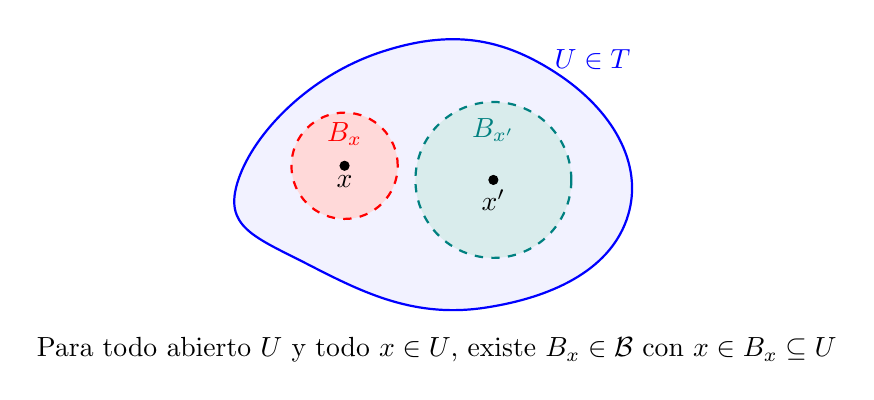
\begin{tikzpicture}[scale=0.9]
    % Abierto U grande
    \draw[thick,blue,fill=blue!5] plot[smooth cycle,tension=0.8] coordinates {(0,0) (2,1.8) (4.5,1.5) (5.5,-0.5) (3.5,-1.8) (1,-1.2)};
    \node[blue] at (5,1.7) {\(U \in \mc T\)};
    
    % Elementos basicos B_x alrededor de puntos
    \draw[thick,red,dashed,fill=red!15] (1.5,0.2) circle (0.75cm);
    \filldraw[black] (1.5,0.2) circle (1.8pt) node[below] {\(x\)};
    \node[red] at (1.5,0.65) {\(B_x\)};
    
    \draw[thick,teal,dashed,fill=teal!15] (3.6,0) circle (1.1cm);
    \filldraw[black] (3.6,0) circle (1.8pt) node[below] {\(x'\)};
    \node[teal] at (3.6,0.7) {\(B_{x'}\)};
    
    \node at (2.8,-2.4) [align=center] {Para todo abierto \(U\) y todo \(x \in U\), existe \(B_x \in \mathcal{B}\) con \(x \in B_x \subseteq U\)};
\end{tikzpicture}
\end{center}

\begin{ejem}
En \((\mathbb{R}, \mc T_d)\):
\begin{itemize}
    \item \(\mathcal{B} = \{B_d(x, \varepsilon) \mid x \in \mathbb{R}, \; \varepsilon > 0\}\) es base.
    \item \(\mathcal{B}_1 = \{(a, b) \mid a < b, \; a, b \in \mathbb{R}\}\) es base.
    \item \(\mathcal{B}_2 = \{(a, b) \mid a < b, \; a, b \in \mathbb{Q}\}\) es base numerable de \(\mc T_d\). Nótese que \(\mathcal{B}_2 \subsetneq \mathcal{B}_1\).
    \item \(\mathcal{B}_3 = \{(a, b) \mid a, b \in \mathbb{R} \setminus \mathbb{Q} = \bb I \}\) es también base.
\end{itemize}
\end{ejem}
Sea $X$ un conjunto
\begin{teo}
Un subconjunto \(\mathcal{B} \subseteq \mathcal{P}(X)\) es base de una topología \(\mc T\) en \(X\) de la cual \(\mathcal{B}\) es base si y solo si \(\mathcal{B}\) satisface:
\begin{enumerate}
    \item[\textbf{1)}] Para todo \(x \in X\), existe \(B_x \in \mathcal{B}\) tal que \(x \in B_x\) (es decir, \(\bigcup_{B \in \mathcal{B}} B = X\)).
    \item[\textbf{2)}] Dados \(B_1, B_2 \in \mathcal{B}\), para cada \(x \in B_1 \cap B_2\) existe \(B_x' \in \mathcal{B}\) tal que \(x \in B_x' \subseteq B_1 \cap B_2\).
\end{enumerate}
Dicha topología \(\mc T\) es única y es $\mc T = <\mc B>$.
\end{teo}

\begin{dem} \, 
\begin{itemize}
    \item[(\(\Rightarrow\))] Sea \(\mc T\) una topología en \(X\) y sea \(\mathcal{B}\) una base de \(\mc T\).
    \begin{itemize}
        \item Como \(X \in \mc T\), para cada \(x \in X\) existe \(B_x \in \mathcal{B}\) tal que \(x \in B_x \subseteq X\). Luego se cumple 1.
        \item Sean \(B_1, B_2 \in \mathcal{B} \subseteq \mc T\). Por ser \(\mc T\) topología, \(B_1 \cap B_2 \in \mc T\). Al ser \(B_1 \cap B_2\) un abierto y \(\mathcal{B}\) base, para cada \(x \in B_1 \cap B_2\) existe \(B_x' \in \mathcal{B}\) tal que \(x \in B_x' \subseteq B_1 \cap B_2\). Luego se cumple 2.
    \end{itemize}
    \item[(\(\Leftarrow\))] Sea $\mc B \subset \mc P(X)$ verificando 1) y 2), se define la familia:
    \[
        \mc T := \{U \subseteq X \mid \forall x \in U, \; \exists B_x \in \mathcal{B} \text{ con } x \in B_x \subseteq U\} \text{}.
    \]
    Veamos que \(\mc T\) es una topología en \(X\):
    \begin{enumerate}
        \item[\textbf{a)}] \(\emptyset \in \mc T\) por definición de $\mc T$. Por la condición 1, para cada \(x \in X\) existe \(B_x \in \mathcal{B}\) con \(x \in B_x \subseteq X\), luego \(X \in \mc T\).
        \item[\textbf{b)}] Sean \(U_1, \ldots, U_n \in \mc T\) y sea \(x \in U_1 \cap \cdots \cap U_n\). Como \(x \in U_i\, \forall i, \ldots, n\), existe \(B_i \in \mathcal{B}\) con \(x \in B_i \subseteq U_i\). Entonces \(x \in B_1 \cap \cdots \cap B_n \subset U_1 \cap \cdots \cap U_n\). Por la condición 2, existe \(B \in \mathcal{B}\) tal que:
        \[
            x \in B \subseteq B_1 \cap \cdots \cap B_n \subseteq U_1 \cap \cdots \cap U_n \text{}.
        \]
        Por consiguiente, \( U_1 \cap \cdots \cap U_n \in \mc T\).
        \item[\textbf{c)}] Sea \(\{U_i\}_{i \in I} \subseteq \mc T\) y sea \(x \in \bigcup_{i \in I} U_i\). Existe \(i_0 \in I\) tal que \(x \in U_{i_0}\). Como \(U_{i_0} \in \mc T\), existe \(B_x \in \mathcal{B}\) tal que:
        \[
            x \in B_x \subseteq U_{i_0} \subseteq \bigcup_{i \in I} U_i \text{}.
        \]
        Por consiguiente, \( \displaystyle \bigcup_{i \in I} U_i \in \mc T\).
    \end{enumerate}
    Así, \(\mc T\) es una topología en \(X\). Además, \(\mathcal{B} \subseteq \mc T\) (tomando \(B_x = B\) para cada \(x \in B\)), y por la propia definición de \(\mc T\), \(\mathcal{B}\) es base de \(\mc T\).
    
    \item[\textbf{Unicidad:}] Si existiera otra topología \(\mc T'\) con base \(\mathcal{B}\), todo abierto de \(\mc T'\) sería unión de elementos de \(\mathcal{B}\) (que pertenecen a \(\mc T\)), luego \(\mc T' \subseteq \mc T\). Recíprocamente, todo abierto de \(\mc T\) es unión de elementos de \(\mathcal{B} \subseteq \mc T'\), luego \(\mc T \subseteq \mc T'\), concluyendo que \(\mc T = \mc T'\).
\end{itemize}
\end{dem}

\begin{obs}
La condición 2 del teorema es equivalente a exigir que para cualesquiera \(B_1, \ldots, B_n \in \mathcal{B}\) y para cada \(x \in \bigcap_{k=1}^n B_k\), existe \(B_x \in \mathcal{B}\) con \(x \in B_x \subseteq \bigcap_{k=1}^n B_k\).
\end{obs}

\begin{dem}
Para \(n = 2\) es la propia condición 2. Supongamos cierto para \(n-1\): si \(x \in \bigcap_{k=1}^n B_k\), entonces \(x \in (\bigcap_{k=1}^{n-1} B_k) \cap B_n\). Por hipótesis de inducción, existe \(B_x^{n-1} \in \mathcal{B}\) con \(x \in B_x^{n-1} \subseteq \bigcap_{k=1}^{n-1} B_k\). Entonces \(x \in B_x^{n-1} \cap B_n\), y aplicando el caso \(n=2\) existen \(B_x \in \mathcal{B}\) con \(x \in B_x \subseteq B_x^{n-1} \cap B_n \subseteq \bigcap_{k=1}^n B_k\).
\end{dem}

\begin{ejer}[Topología de Sorgenfrey o del límite inferior]
En \(\mathbb{R}\), consideremos la familia de intervalos semiabiertos \(\mathcal{B} = \{[a, b) \mid a < b, \; a, b \in \mathbb{R}\} \subset \mathcal{P}(\mathbb{R})\). Se verifican las condiciones del teorema
\begin{enumerate}
    \item[\textbf{1)}] Para todo \(x \in \mathbb{R}\), \(x \in [x, x+1) \in \mathcal{B}\).
    \item[\textbf{2)}] Dados \([a, b), [a', b') \in \mathcal{B}\), su intersección es:
    \[
        [a, b) \cap [a', b') = \begin{cases} \emptyset & \text{si } \max\{a, a'\} \ge \min\{b, b'\}, \\ [\max\{a, a'\}, \min\{b, b'\}) \in \mathcal{B} & \text{si } \max\{a, a'\} < \min\{b, b'\}. \end{cases} \text{}
    \]
\end{enumerate}
Por tanto, \(\mathcal{B}\) es base de una topología en \(\mathbb{R}\), denotada \(\mc T_{\text{Sorg}}\) (o \(\mathbb{R}_l\)). Se verifica que \(\mc T_d \subsetneq \mc T_{\text{Sorg}}\), puesto que todo intervalo abierto usual es unión de intervalos de \(\mathcal{B}\):
\[
    (a, b) = \bigcup_{n=1}^\infty \left[a + \frac{1}{n}, b\right) \in \mc T_{\text{Sorg}} \text{},
\]
mientras que \([a, b) \notin \mc T_d\).

Sabemos que $\mc T_d=<\mc B>$, siendo $\mc B=\{(a,b), \, / \,  a,b \in \bb R\}$. Si demostramos que $\mc B \subset \mc T_{Sorg}\Rightarrow <\mc B>=\mc T_d \subseteq \mc T_{Sorg}$ (\textbf{Observaci\'on:} La diferencia entre $\mc B$ y $<\mc B>$ es que en $<\mc B>$ est\'an las uniones arbitrarias). 

Sea $(a,b)\in \mc T_d$ veamos si $(a,b)\in \mc T_{Sorg} \iff \forall \, x\in (a,b) \, \exists \, B_x\subset \mc B_{Sorg}\, / \, x\in B_x \subset(a,b)$. Queremos encontrar un intervalo de la forma $[\,\,)$ que contenga a $x$ y est\'e contenido en $(a,b)$. 

Sea $x\in (a,b) \Rightarrow x\neq b \Rightarrow b-x = \varepsilon'>0, \, \varepsilon = \frac{\varepsilon}{2}$. As\'i $[x,x+\varepsilon)=B\subset (a,b)$ es el intervalo que busc\'abamos ya que $x\in B \subset(a,b)$. 

Por tanto, $[a,b) \in \mc T_{Sorg}$ pero $[a,b)\nin \mc T_d$.

Para la otra inclusi\'on basta ver que no se cumple si encontramos un elementos de $\mc T_{Sorg}$ que no est\'a en $\mc T_d$ (trivial). 
\end{ejer}
\begin{ejer}
Si $\mc B$ es base de una topolog\'ia en $X$, entonces $<\mc B>$ es la menor topolog\'ia de $X$ que contiene a $\mc B$.
\end{ejer}
\begin{ejer}
Ya sabemos que $\mc T_d\subset \mc T_{Sorg}$ y que $[a,b)\in \mc T_{Sorg}$. ¿$(-\infty,a), (-\infty,a], (b,\infty), [b,\infty)$ son abiertos, cerrados o ambos por la $\mc T_{Sorg}$? 
\begin{itemize}
    \item $(-\infty, a) \in \mc T_d \Rightarrow (-\infty, a) \in \mc T_{Sorg}$ pues $\mc T_d\subset \mc T_{Sorg}$
    \item $(-\infty,a]$. $\forall \, x\in (-\infty,a] \, \exists [\,\,)\, / \, x\in [\,\,) \subset(-\infty,a]?$
    
    Para $a\in (-\infty,a], \, [a,a+\varepsilon) \nsubseteq (-\infty,a]\Rightarrow $ no abierto.
    \item $(b,\infty) \in \mc T_d \Rightarrow (b,\infty)\in \mc T_{Sorg}$.
    \item $[b,\infty)\, \forall \, x\in [b,\infty)\, \exists\,[x,x+1) \, / \, x \in [x,x+1) \subset [b, \infty) \Rightarrow $ es abierto.
    
    Veamos si son cerrados
    \item  $(-\infty,a)^c=[a,\infty)$ es abierto para $\mc T_S \Rightarrow (-\infty,a)$ es cerrado.
    \item $(-\infty,a]^c = (a,\infty)$ es abierto para $\mc T_S \Rightarrow (-\infty,a]$ es cerrado.
    \item $(b,\infty)^c = (-\infty,b]$ no abierto $\Rightarrow (b,\infty)$ no cerrado.
    \item $[b,\infty)^c = (-\infty, b)$ es abierto $\Rightarrow [b,\infty)$ es cerrado.
\end{itemize}
Tenemos pues, por definici\'on, $[a,b)$ son abiertos para $\mc T_{Sorg}$. Sus complementarios son $(-\infty,a) \cup [b,\infty)$ abiertos por ser ambos abiertos, luego $[a,b)$ son cerrados. 

\underline{Conclusi\'on}: $[a,b)$ son abiertos y cerrados.

En cambio, $(a,b]$ no es abierto para $\mc T_{Sorg}$ pues $(a,b]^c = \underbrace{(-\infty,a]}_{no \, ab.}\cup \underbrace{(b,\infty)}_{ab.}$ no es abierto, debido al punto $a\in (-\infty,a]\cup [b,\infty)$ (NO porque no ab $\cup$ ab no sea abierto, lo podr\'ia llegar ser).

\underline{Conclusi\'on}: $(a,b]$ no son abiertos ni cerrados.
\end{ejer}
\begin{ejer}
    Sea $\mc T \subset \mc T'$ dos topolog\'ias en $X$, entonces todo abierto por $\mc T$ es abierto por $\mc T'$. Demostrar que si $C \subset X$ es cerrado por $\mc T$, entonces es cerrado por $\mc T'$. 
\end{ejer}
\begin{sol}
En 1 l\'inea. OJO: $\mc P(X) - \mc T \neq \mc C_{\mc T}$
\end{sol}
\section{Topología por cerrados}

Sea \((X, \mc T)\) un espacio topológico. La familia de cerrados se define como \(\mathcal{C}_\mc T := \{X \setminus U \mid U \in \mc T\} \subseteq \mathcal{P}(X)\), es decir, el conjunto de los complementarios de los abiertos de la topología $\mc T$.

\begin{prop}
La familia \(\mathcal{C}_\mc T\) verifica las siguientes propiedades:
\begin{enumerate}
    \item[\textbf{1)}] \(\emptyset, X \in \mathcal{C}_\mc T\).
    \item[\textbf{2)}] Si \(C_1, \ldots, C_n \in \mathcal{C}_\mc T \Rightarrow C_1 \cup \ldots \cup C_n \in \mathcal{C}_\mc T\) (uniones finitas de cerrados son cerradas).
    \item[\textbf{3)}] Si \(\{C_i\}_{i \in I} \subseteq \mathcal{C}_\mc T \Rightarrow \bigcap_{i \in I} C_i \in \mathcal{C}_\mc T\) (intersecciones arbitrarias de cerrados son cerradas).
\end{enumerate}
\end{prop}

\begin{dem}
\begin{enumerate}
    \item[\textbf{1)}] \(\emptyset = X \setminus X\) con \(X \in \mc T\), y \(X = X \setminus \emptyset\) con \(\emptyset \in \mc T\), luego \(\emptyset, X \in \mathcal{C}_\mc T\).
    \item[\textbf{2)}] Sean \(C_1, \ldots, C_n \in \mathcal{C}_\mc T\). Existen \(U_1, \ldots, U_n \in \mc T\) tales que \(C_k = X \setminus U_k\). Por las leyes de De Morgan:
    \[
        \bigcup_{k=1}^n C_k = \bigcup_{k=1}^n (X \setminus U_k) = X \setminus \left(\bigcap_{k=1}^n U_k\right) \text{}.
    \]
    Como \(\mc T\) es topología, \(\bigcap_{k=1}^n U_k \in \mc T\), y su complementario pertenece a \(\mathcal{C}_\mc T\).
    \item[\textbf{3)}] Sea \(\{C_i\}_{i \in I} \subseteq \mathcal{C}_\mc T\), con \(C_i = X \setminus U_i\) para \(U_i \in \mc T\). Por las leyes de De Morgan:
    \[
        \bigcap_{i \in I} C_i = \bigcap_{i \in I} (X \setminus U_i) = X \setminus \left(\bigcup_{i \in I} U_i\right) \text{}.
    \]
    Como \(\bigcup_{i \in I} U_i \in \mc T\), su complementario pertenece a \(\mathcal{C}_\mc T\).
\end{enumerate}
\end{dem}
\begin{obs}
    Para ciertas topolog\'ias es mucho m\'as c\'omodo hablar en t\'erminos de cerrados.
    \begin{itemize}
        \item $\mc C_{\mc T_{cof}} = \{A\subset X \, / \, A \text{ es finito}\} \cup \{X\}$
        \item $\mc C_{\mc T_{cocont}} = \{A\subset X \, / \, A \text{ es contable}\} \cup \{X\}$
    \end{itemize}
\end{obs}
\begin{ejem}
\begin{enumerate}
    \item Sea $X=\{a,b,c\}$ nuestro conjunto, si $\mc T=\{\emptyset, X, \{a\},\{b,c\}\}$ es nuestra topolog\'ia por abiertos de $X$, $\mc C_{\mc T} = \{X, \emptyset,\{b,c\},\{a\}\}$ es nuestra topol\'ia por cerrados.
    
    En $(X,\mc T)$ los abiertos y cerrados son los mismos subconjuntos y hay subconjuntos que no son ni abiertos ni cerrados, como por ejemplo $\{a,b\}$.
    \item Sea $(\bb R, \mc T_d)$,
    \begin{itemize}
        \item $(a,b) \in \mc T_d$
        \item $[a,b] \in \mc C_{\mc T_d}$ pues $\bb R - [a,b] = (-\infty,a) \cup(b,\infty) \in \mc T_d$. Adem\'as, $[a,b]\nin \mc T_d$ pues tomando $a\in [a,b] \, \nexists \, B(a, \varepsilon) \subset [a,b]$.
        \item Por tanto, $ [a,b],[a,b),(a,b] \nin \mc T_d$
        \item Adem\'as, haciendo complementarios $(a,b] \nin \mc C_{\mc T_d}, \, [a,b) \nin \mc C_{\mc T_d}, \, (-\infty, a] \nin \mc C_{\mc T_d}$
        \item $\{0\}^c=(-\infty,0) \cup (0,\infty) \Rightarrow 0 \in \mc C_{\mc T_d}$ es decir, que el complementario de cualquier $x\in \bb R$ es uni\'on de dos abiertos, por lo tanto abierto, y esto nos dice que $\{x\}$ es cerrado en $(\bb R, \mc T_d)$.
    \end{itemize}
\end{enumerate}
\end{ejem}

\begin{teo}
Sea \(X\) un conjunto y sea \(\mathcal{C} \subseteq \mathcal{P}(X)\) una familia de subconjuntos. Existe una (única) topología \(\mc T\) por abiertos en \(X\) tal que \(\mathcal{C}_\mc T = \mathcal{C}\) si y solo si \(\mathcal{C}\) satisface las condiciones 1, 2 y 3 de la proposición anterior.
\end{teo}

\begin{dem}
Si \(\mathcal{C}\) verifica las tres condiciones, definiendo \(\mc T := \{X \setminus C \mid C \in \mathcal{C}\}\), al tomar complementarios las tres condiciones de \(\mathcal{C}\) se traducen directamente (por De Morgan) en los tres axiomas de topología por abiertos de la Definición 1.1.
\end{dem}

\begin{defi}
Sea \((X, \mc T)\) un espacio topológico y \(\mathcal{C}\) su familia de cerrados. Una subfamilia \(\mathcal{B}_{\text{cerr}} \subseteq \mathcal{C}\) es una \textbf{base de cerrados} si para todo cerrado \(C \in \mathcal{C}\) y todo punto \(x \notin C\), existe un elemento básico \(B_x \in \mathcal{B}_{\text{cerr}}\) tal que:
\[
    C \subseteq B_x \quad \text{y} \quad x \notin B_x \text{}.
\]
Equivalentemente, todo cerrado \(C \in \mathcal{C}\) es intersección de elementos de \(\mathcal{B}_{\text{cerr}}\): \(C = \bigcap_{i \in I} B_i\) con \(B_i \in \mathcal{B}_{\text{cerr}}\).
\end{defi}

\begin{center}
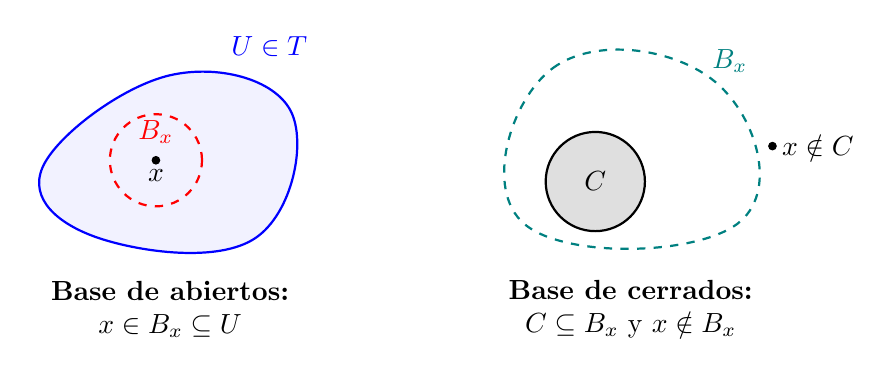
\begin{tikzpicture}[scale=0.9]
    % Base por abiertos
    \begin{scope}[shift={(0,0)}]
        \draw[thick,blue,fill=blue!5] plot[smooth cycle,tension=0.7] coordinates {(0,0) (1.8,1.3) (3.5,0.8) (3,-1) (0.8,-1)};
        \node[blue] at (3.2,1.7) {\(U \in \mc T\)};
        \draw[thick,red,dashed] (1.6,0.1) circle (0.65cm);
        \filldraw[black] (1.6,0.1) circle (1.5pt) node[below] {\(x\)};
        \node[red] at (1.6,0.5) {\(B_x\)};
        \node at (1.8,-2) [align=center] {\textbf{Base de abiertos:} \\ \(x \in B_x \subseteq U\)};
    \end{scope}
    
    % Base por cerrados
    \begin{scope}[shift={(7,0)}]
        \draw[thick,fill=gray!25] (0.8,-0.2) circle (0.7cm);
        \node at (0.8,-0.2) {\(C\)};
        \draw[thick,teal,dashed] plot[smooth cycle,tension=0.8] coordinates {(-0.2,-0.8) (0.2,1.4) (2.5,1.2) (2.8,-0.8)};
        \node[teal] at (2.7,1.5) {\(B_x\)};
        \filldraw[black] (3.3,0.3) circle (1.5pt) node[right] {\(x \notin C\)};
        \node at (1.3,-2) [align=center] {\textbf{Base de cerrados:} \\ \(C \subseteq B_x\) y \(x \notin B_x\)};
    \end{scope}
\end{tikzpicture}
\end{center}

\section{Subbases de una topología}

\begin{defi}
Un subconjunto \(S\mc B \subseteq \mathcal{P}(X)\) es una \textbf{subbase} de una topología en \(X\) si cubre a \(X\): para todo \(x \in X\) existe \(S \in S\mathcal{B}\) tal que \(x \in S\) (\(X = \bigcup_{S \in S\mathcal{B}} S\)).
\end{defi}

La base generada por \(S\mathcal{B}\) es la familia de todas las intersecciones finitas:
\[
    S\mc B \subset \mathcal{B}_{S\mathcal{B}} = \{B\subset X \, / \, B=S_1 \cap \ldots \cap S_n \mid S_j \in S\mathcal{B}, \; n \in \mathbb{N}\} \text{},
\]
base de una topolog\'ia y la topología generada por \(S\mathcal{B}\) es:
\[
    \mc T_{S\mathcal{B}}  = \mc T_{\mc B_{S\mc B}} = <\mc B_{S\mc B}> = \left\{\bigcup_{j \in J} (V_{j, 1} \cap \ldots \cap V_{j, n_j}) \;\middle|\; V_{j, r} \in \mathcal{S}\right\} \cup \{\emptyset\} \text{}.
\] es decir, las uniones arbitrarias de intersecciones finitas de elementos de $S\mc B$. 

\begin{ejem}
En \(\mathbb{R}\):
\begin{itemize}
    \item \(S\mathcal{B} := \{(-\infty, b), (a, \infty) \mid a, b \in \mathbb{R}\}\) es subbase de la topología usual \(\mc T_d\): para cada \(x \in \mathbb{R}\), \(x \in (x - 1, \infty) \in \mathcal{S}\). Además, \((a, b) = (-\infty, b) \cap (a, \infty) \in \mathcal{B}_{S\mathcal{B}}\), lo que genera la base de intervalos usual y demuestra que \(\mc T_{S\mathcal{B}} = \mc T_d\).
    \item \(S\mathcal{B}' := \{(-\infty, b], [a, \infty) \mid a, b \in \mathbb{R}\}\) es subbase de la topología discreta \(\mc T_{\text{discreta}}\), ya que considerando $x \in \bb R$ buscamos un abierto de la subbase que lo contenga \(\{x\} = (-\infty, x] \cap [x, \infty) \in \mathcal{B}_{S\mathcal{B}'}\), haciendo que todos los conjuntos unitarios sean abiertos, lo que demuestra que $<S\mc B'>= \mc T_{disc}$. Pues $Y = \displaystyle \bigcup_{y\in Y} \{y\}$ cada subconjunto es uni\'on de sus puntos.
\end{itemize}
\end{ejem}

\section{Bases y subbases de una topolog\'ia por cerrados}
Todas las demostraciones son pasando al complementario.

Sea $(X,\mc C)$ esapcio topolo\'ogico por cerrados. \begin{defi}
    $\mc B \subset \mc P(X)$ es un \textbf{base por cerrados} (o \textbf{base de $\mc C$}) si para todo cerrado $C$ y para todo $x\nin C$, existe $B \in \mc B$ tal que $x\nin B \supset C \iff X \neq C =\displaystyle \bigcap_{B_i \in \mc B} B_i$, es decir, todo cerrado es intersecci\'on de cerrados de la base. 
\end{defi}
\begin{defi} La base $\mc B$ genera una topolog\'ia por abiertos 
    $$\mc C_{\mc B} = <\mc B> = \{C \subset X \, / \, \forall x \nin C, \text{ existe } B_x \in \mc B \, / \, x \nin B_x \supset C\}  =\left\{\bigcap_{B_i \in \mc B} B_i \right\}\cup \{X\}$$
    Los cerrados de una base de $\mc C$ se llaman \textbf{cerrados básicos}, y son los complementarios de los abiertos b\'asicos.

\end{defi}
\begin{prop}
Si $X$ es conjunto, $\mc B \subset \mc P(X)$, $\mc B$ es una base por cerrados si y solo si
\begin{enumerate}
    \item $\forall\, x\in X$, existe $b\in \mc B$ tal que $x\nin B$.
    \item $\forall \, B_1,B_2 \in \mc B$ y prar todo $X\in B_1\cup B_2$, existe $B_x\in \mc B$ tal que $x \nin B_x \supseteq B_1\cap B_2$.
\end{enumerate}
\end{prop}
\begin{defi}
    Una \textbf{subbase por cerrados} $S\mc B$ es un subconjunto $S\mc B\subset \mc P(X)$ que verifica 
    \begin{enumerate}
        \item $\forall \, x\in X$, existe $S\in S\mc B$ tal que $x\nin S$. $\mc B_{S\mc B}$
        \item $<\mc B_{S\mc B}> = \mc T_{S\mc B}$ con $\mc B_{S\mc B} := \{S_1\cup \cdots \cup S_n \, / \,S_i\in S\mc B \}$, es decir, son uniones finitas de intersecciones arbitrarias. 
    \end{enumerate}
\end{defi}
\section{Elementos de un espacio topol\'ogico}
Sea $X$ un espacio topol\'ogico y sea $Y\subseteq X$ un subconjunto
\begin{defi} El \textbf{interior} de un subconjunto $Y\subset X$ es el mayor abierto de $X$ contenido en $Y$:
    $$Y^{\circ} = \{y\in Y \, / \, \text{ existe un abierto } U_y \text{ tal que } y\in U_y \subset Y\} = \bigcup_{U\subset Y} U$$
    Siempre existe $\emptyset$ lo verifica y es abierto en $X$. Adem\'as, si $V \subseteq X$ es abierto, $V\subset Y \Rightarrow V \subseteq Y^{\circ}$.
\end{defi}
\begin{defi}
El \textbf{cierre} (o \textbf{clausura} o \textbf{adherencia}) de un subconjunto $Y \subseteq X$ es el menor cerrado de $X$ que contiene a $Y$:
\[
    \overline{Y} := \bigcap_{\substack{Y \subseteq C \\ C \in \mathcal{C}_\mc T}} C.
\]
Se cumple que $Y \subseteq \overline{Y}$. 
\end{defi}
\begin{prop}
\[
    \overline{Y} = \{x \in X \mid \text{ para todo abierto } U_x \text{ se verifica que } U_x \cap Y \ne \emptyset\}.
\]
\end{prop}
\begin{dem}
\begin{itemize}
    \item[($\subseteq$)] Sea $x \in \overline{Y}$ y sea $U_x$ un abierto con $x \in U_x$. Supongamos que $U_x \cap Y = \emptyset$. Entonces $Y \subseteq X \setminus U_x$. Como $X \setminus U_x$ es cerrado, por definición de cierre $\displaystyle \overline{Y} = \bigcap_{\substack{C' cualquiera \\ C' \supset Y}} C ' \subseteq C' \Rightarrow x \in X \setminus U_x$, contradiciendo que $x \in U_x$. Por tanto, $U_x \cap Y \ne \emptyset$.
    \item[($\supseteq$)] Veamos que $x\in \overline Y = \bigcap C \iff x\in C \, / \, \forall C \supset Y$. Sea $C$ cerrado, $C\supset Y$ y supongamos que $x\nin C \Rightarrow x \in X-C = U$ abierto. Como $Y\subset C$, $X-C \cap Y=\emptyset$. Por definci\'on del cierre, $U\cap Y = \emptyset$ llegando a contradicci\'on, al suponer que $x\nin C$.
\end{itemize}
\end{dem}
\begin{defi}
    Sea $Y\subset X$, se llaman \textbf{puntos de acumulación} al subconjunto:
    $$Y' = \{x\in X \mid \text{para todo abierto } U_x \text{ con } x\in U_x, \, U_x \cap Y \neq \emptyset, \{x\}\}$$

\end{defi}
\begin{obs}
    $Y' \subset \overline{Y}$ (ejercicio).
\end{obs}
\begin{defi}Se definen los \textbf{puntos aislados} de $Y$ como
    $$Y^a = \{y\in Y \mid \text{ existe un abierto } U_y, y\in U_y \text{ tal que } U_y \cap Y = \{y\} \} = \{y \in Y \mid y \in Y'\}\subset Y$$
\end{defi}
\begin{defi}
    Se define la \textbf{frontera} de $Y$ como 
    $$Fr(Y) = \overline{Y} \cap \overline{(X-Y)}$$
\end{defi}
\begin{defi}
    Se define el \textbf{borde} de $Y$ como 
    $$b(Y) = Y \cap Fr(Y) = Y \cap \overline{(X-Y)}$$ 
\end{defi}
\begin{defi}
    Se define el \textbf{exterior} de $Y$ como 
    $$Ext(Y)=(X-Y)^{\circ}$$
\end{defi}
\begin{propis}
\begin{enumerate}
    \item $\overline{Y} = Y \cup Y' = Y^a \sqcup Y'$
    \begin{dem}
        $\subseteq) $ Sea $x\in \overline{Y}$, 

        Si $x\in Y$, hemos acabado.

        Si $x\nin Y$, por ser $x\nin \overline{Y} \Rightarrow \forall\, U_x$ abierto, $U_x\cap Y \neq \emptyset$ y $U_x\cap Y \neq x$ pues $x\nin Y \Rightarrow x\in Y' \Rightarrow x\in Y \cup Y'$

        $\supseteq)$ Como $Y \subset \overline{Y}$ y $Y' \subset \overline{Y} \Rightarrow Y \cup Y' \subset \overline{Y}$, luego
        $$Y\cap Y' = Y-Y^a \Rightarrow \overline{Y} = Y^a \cup Y' = Y^a \sqcup Y'$$
    \end{dem}
    \item $Y^{\circ} \cap b(Y) = \emptyset$
    \begin{dem}
        Sea $x\in Y^{\circ} \Rightarrow x \overset{?}{\nin} b(Y)$

        $x\in Y^{\circ} \Rightarrow$ existe $U_x$ abierto con $x\in U_x \subset Y \Rightarrow x\nin b(Y) \Rightarrow Y^{\circ} \cap b(Y) = \emptyset$
    \end{dem}
    \item $Y^{\circ} \cap Fr(Y) = \emptyset$ (se deduce de lo anterior)
    
    $Y^{\circ} \cap b(Y)  = Y^{\circ} \cap Fr(Y)$ porque $Y^{\circ} \subseteq Y$.
\end{enumerate}
\end{propis}



\begin{ejem}
En $(\mathbb{R}, \mc T_d)$, sea $Y = [0, 1)$:
\begin{itemize}
    \item $Y^\circ = (0, 1)$, $\overline{Y} = [0, 1]$, $Y' = [0, 1]$, $Y^a = \emptyset$.
    \item $X \setminus Y = (-\infty, 0) \cup [1, \infty)$, $\overline{X \setminus Y} = (-\infty, 0] \cup [1, \infty)$.
    \item $\operatorname{Fr}(Y) = \{0, 1\}$.
    \item $b(Y) = \{0\}$.
    \item $\operatorname{Ext}(Y) = (-\infty, 0) \cup (1, \infty)$.
\end{itemize}
\end{ejem}

\begin{ejem}
En $\mathbb{R}^2$ con la topología usual, sea $Y = [1, 3) \times [1, 2) \cup \{(4, 1), (5, 1)\}$:
\begin{itemize}
    \item $Y^\circ = (1, 3) \times (1, 2)$.
    \item $\overline{Y} = [1, 3] \times [1, 2] \cup \{(4, 1), (5, 1)\}$.
    \item $Y' = [1, 3] \times [1, 2]$.
    \item $Y^a = \{(4, 1), (5, 1)\}$.
\end{itemize}
\end{ejem}
\begin{prop}
    $Y$ es cerrado $\iff Fr(Y) \subset Y$.
\end{prop}
\begin{dem}
    $\Rightarrow) \, Y$ cerrado $\Rightarrow Y = \bar Y \supset Fr(Y) \Rightarrow Fr(Y) \subset Y$

    $\Leftarrow)$ Sabemos que $\bar Y = Y^{\circ} \sqcup Fr(Y)\subset Y$ (pues $Y^{\circ}, Fr(Y)\subset Y$). Luego
    $$\overline{Y} = Y^{\circ} \sqcup Fr(Y) \subset Y \subset \overline{Y} \Rightarrow Y = \overline{Y} \Rightarrow Y \text{ es cerrado.}$$
\end{dem}

\section{Propiedades fundamentales de los operadores}

\begin{propi}
Sean $X$ un espacio topológico e $Y \subseteq X$. Se verifican:
\begin{enumerate}
    \item[\textbf{I.}] $Y^\circ \cap \operatorname{Fr}(Y) = \emptyset$.
    \item[\textbf{II.}] $\operatorname{Ext}(Y) \cap \operatorname{Fr}(Y) = \emptyset$.
    \item[\textbf{III.}] $Y^\circ \cap b(Y) = \emptyset$.
    \item[\textbf{IV.}] $Y = Y^\circ \sqcup b(Y)$.
    \item[\textbf{V.}] $\overline{Y} = Y^\circ \sqcup \operatorname{Fr}(Y)$.
    \item[\textbf{VI.}] $Y$ es abierto $\iff b(Y) = \emptyset$.
    \item[\textbf{VII.}] $Y$ es cerrado $\iff \operatorname{Fr}(Y) \subseteq Y$.
    \item[\textbf{VIII.}] $\operatorname{Ext}(Y) = X \setminus \overline{Y}$.
    \item[\textbf{IX.}] $\overline{X \setminus Y} = X \setminus Y^\circ$.
    \item[\textbf{X.}] $\overline{Y^\circ} \subseteq \overline{Y}$ (en general no se da la igualdad).
    \item[\textbf{XI.}] $Y^\circ \subseteq (\overline{Y})^\circ$ (en general no se da la igualdad).
\end{enumerate}
\end{propi}

\begin{dem}
\begin{itemize}
    \item[\textbf{I.}] $Y^\circ \cap \operatorname{Fr}(Y) = Y^\circ \cap (\overline{Y} \cap \overline{X \setminus Y}) = Y^\circ \cap \overline{X \setminus Y} = \emptyset$, pues si $y \in Y^\circ$, existe un abierto $U_y \subseteq Y$, con lo cual $U_y \cap (X \setminus Y) = \emptyset$, lo que implica $y \notin \overline{X \setminus Y}$.
    \item[\textbf{II.}] $\operatorname{Ext}(Y) \cap \operatorname{Fr}(Y) = (X \setminus Y)^\circ \cap \operatorname{Fr}(X \setminus Y) = \emptyset$ aplicando la propiedad I a $X \setminus Y$.
    \item[\textbf{III.}] $Y^\circ \cap b(Y) = Y^\circ \cap (Y \cap \operatorname{Fr}(Y)) = Y^\circ \cap \operatorname{Fr}(Y) = \emptyset$.
    \item[\textbf{IV.}] Si $y \in Y$, o bien $y \in Y^\circ$, o bien para todo abierto $U \ni y$ se tiene $U \not\subseteq Y$, es decir, $U \cap (X \setminus Y) \ne \emptyset$, lo que implica $y \in \overline{X \setminus Y}$; luego $y \in Y \cap \overline{X \setminus Y} = b(Y)$. La unión es disjunta por III.
    \item[\textbf{V.}] Análoga a IV usando $\overline{Y}$ y $\operatorname{Fr}(Y)$.
    \item[\textbf{VI.}] $Y$ es abierto $\iff Y = Y^\circ \iff b(Y) = Y \setminus Y^\circ = \emptyset$.
    \item[\textbf{VII.}] $Y$ es cerrado $\iff X \setminus Y$ es abierto $\iff b(X \setminus Y) = \emptyset \iff (X \setminus Y) \cap \operatorname{Fr}(Y) = \emptyset \iff \operatorname{Fr}(Y) \subseteq Y$.
    \item[\textbf{VIII.}] $x \in \operatorname{Ext}(Y) \iff x \in (X \setminus Y)^\circ \iff \exists U_x \text{ abierto con } U_x \subseteq X \setminus Y \iff U_x \cap Y = \emptyset \iff x \notin \overline{Y} \iff x \in X \setminus \overline{Y}$.
    \item[\textbf{IX.}] Tomando complementarios en VIII: $\overline{X \setminus Y} = X \setminus (X \setminus (X \setminus Y))^\circ = X \setminus Y^\circ$.
    \item[\textbf{X.}] Como $Y^\circ \subseteq Y \Rightarrow \overline{Y^\circ} \subseteq \overline{Y}$. En $(\mathbb{R}, \mc T_d)$, para $\mathbb{Q}$ se tiene $\mathbb{Q}^\circ = \emptyset \Rightarrow \overline{\mathbb{Q}^\circ} = \emptyset \ne \mathbb{R} = \overline{\mathbb{Q}}$.
    \item[\textbf{XI.}] Como $Y^\circ$ es un abierto contenido en $Y \subseteq \overline{Y}$, necesariamente $Y^\circ \subseteq (\overline{Y})^\circ$. Para $\mathbb{Q}$ en $\mathbb{R}$: $\mathbb{Q}^\circ = \emptyset$, pero $(\overline{\mathbb{Q}})^\circ = \mathbb{R}^\circ = \mathbb{R}$.
\end{itemize}
\end{dem}

\section{Subconjuntos densos y clausura relativa}

\begin{defi}
Sea $X$ un espacio topológico e $Y \subseteq X$. Se dice que $Y$ es \textbf{denso} en $X$ si su cierre es el espacio total:
\[
    \overline{Y} = X.
\]
\end{defi}

\begin{prop}
Un subconjunto $Y \subseteq X$ es denso $\iff$ todo abierto no vacío $U \subseteq X$ corta a $Y$ ($U \cap Y \ne \emptyset$).
\end{prop}

\begin{dem}
($\Rightarrow$) Sea $U \ne \emptyset$ abierto en $X$. Sea $x \in U$. Como $X = \overline{Y}$, $x \in \overline{Y}$, por lo que todo entorno abierto de $x$ corta a $Y$; en particular, $U \cap Y \ne \emptyset$.

($\Leftarrow$) Sea $x \in X$. Todo abierto $U \ni x$ es no vacío, luego corta a $Y$, de donde $x \in \overline{Y}$. Por tanto, $X \subseteq \overline{Y} \Rightarrow \overline{Y} = X$.
\end{dem}

\begin{prop}
Sea $Y \subseteq X$ un subespacio topológico y sea $Z \subseteq Y$. Denotemos por $\overline{Z}^X$ la clausura de $Z$ en $X$. Entonces $Z$ es cerrado en $Y$ si y solo si:
\[
    Z = \overline{Z}^X \cap Y.
\]
\end{prop}

\begin{dem}
Si $Z$ es cerrado en $Y$, existe un cerrado $C \subseteq X$ tal que $Z = C \cap Y$. Como $Z \subseteq C$ y $C$ es cerrado en $X$, $\overline{Z}^X \subseteq C$. Por ende, $Z \subseteq \overline{Z}^X \cap Y \subseteq C \cap Y = Z$, de modo que $Z = \overline{Z}^X \cap Y$. El recíproco es inmediato, ya que $\overline{Z}^X$ es cerrado en $X$.
\end{dem}
\begin{ejem}
    $\bb Q$ es denso en $\bb R$.
\end{ejem}
\begin{ejem}
    Sea $(\bb R, \mc T_{kol})$, siendo $\mc T_{kol} = \{\emptyset, \bb R\} \cup \{(a,\infty), \, a \in \bb R\}$, consideremos $Y = \{0\} \cup [1,\infty)$. Tenemos que $\mc C_{\mc T_{kol}}= \{\emptyset, \bb R\} \cup\{(-\infty, a] , \, a\in \bb R\}$. Calculemos $Y$ aplicando operadores.
    \begin{itemize}
        \item $Y^{\circ} = (1, \infty)$. Por reducción al absurdo. Sea $b \in Y \subset (-\infty, a], b+(a-b)+2000 \in Y$ pero $b+(a-b)+2000 \nin (-\infty, a]$. 
        \item $X-Y = (-\infty, 0) \cup (0,1)$.
        \item $\overline{Y} = \bb R$. TERMINAR DE CALCULAR EL RESTO. 
    \end{itemize}
\end{ejem}



\section{Subespacios topol\'ogicos}

Sea \((X, \mc T_X)\) un espacio topológico y sea \(Y \subseteq X\) un subconjunto. Se tiene la aplicaci\'on inclusi\'on
$$\bt Y \rar[hook]{i} & X \\[-5mm] y \rarmaps & y \et$$
de forma que se induce la aplicaci\'on 
$$\bt \mc P(X) \rar[hook]{i^*} & \mc P(Y) &[-11mm] \\[-5mm]
 A \rarmaps & i^*(A) &[-12mm] = i^{-1}(A) = A \cap Y  \\[-5mm] 
 \mc T_X \rarmaps & i^*(\mc T_X) &[-11mm] = \{V \subset Y: \text{existe } &[-11mm] U \in \mc T_X \text{ tal que } i^*(U)=U\cap Y=V\} =:\mc T_X |_Y
\et$$
\begin{prop}
    $\mc T_X|_Y$ es una topolog\'ia en $Y$. 
\end{prop}\begin{dem}
    Por las propiedades de $i^*$. 
\end{dem}
\begin{defi}
Se tiene que $(Y, \mc T_X|_Y)$ es un espacio topol\'ogico, y decimos que $Y\subset (X,\mc T_X)$ es un \textbf{subespacio topológico} si en $Y$ tenemos la topolog\'ia $\mc T_X|_Y$. 
\end{defi}
\begin{defi}
    $V$ es \textbf{abierto en $Y$} si existe un abierto $U$ de $X$ tal que $U\cap Y = V$ (igual para cerrados por la intersecci\'on de complementarios). 
\end{defi}
\begin{obs}
    ¿Es $V$ abierto en $X$? Solo si $Y\subset X$ es abierto en $X$. Igual para cerrados. Diremos que abierto de abierto es abierto en el ambiente $X$ y cerrado de cerrado es cerrado en el ambiente. 
\end{obs}
\begin{ejer}
    Sea $Z \subset Y$, se verifica que $Z$ es cerrado si y solo si $\overline{Z^X} \cap Y = Z$.  
\end{ejer}
\begin{dem}
    (Nota: no es el \'unico cerrado que lo verifica pero es el menor cerrado de $X$ que lo verifica)

    $\Rightarrow) $ $Z$ cerrado en $Y \Rightarrow$ existe $C\subset X$ tal que $C\cap Y = Z \Rightarrow Z \subset C$ y como $Z \subset \overline{Z^X}$, $\overline{Z^X}\subset C \Rightarrow Z \cap Y = Z \subset \overline{Z^X} \cap Y \subset C \cap Y =Z\Rightarrow \overline{Z^X} \cap Y = Z$.
    
    $\Leftarrow)$ Existe $\overline{Z^X}$ cerrado en $X$ tal que $\overline{Z^X} \cap Y =Z \Rightarrow Z$ es cerrado en $Y$.
\end{dem}
\begin{prop}
    Un punto $y\in Y$ es \textbf{aislado en $Y$} $\iff \{y\} \subset Y$ es abierto en $Y$.
\end{prop}
\begin{dem}
    $y \in Y$ es aislado en $Y \,\iff \, $ existe un abierto $U \subset X$ tal que $U\cap Y = \{y\} \iff \{y\}$ es abierto en $Y$.
\end{dem}
\begin{prop}
    Sea $(X, \mc T_X)$ espacio topol\'ogico. Entonces un subconjunto $A\subset X$ es abierto en $X\, \iff \, $ para todo $x\in A$ existe un abierto $U_X \in \mc T_X$ tal que $x\in U_x\subset A \, \iff \, x\in A^{\circ} \, \forall \, x \in A \, \iff \, A = A^{\circ} \, \iff \, A \text{ es abierto. }$
\end{prop}

\section{Entornos}
\begin{defi}
Sea \((X, \mc T)\) un espacio topológico y sea \(x \in X\). Un subconjunto \(V \subseteq X\) es un \textbf{entorno} del punto \(x\) si existe un abierto \(U \in \mc T\) tal que:
\[
    x \in U \subseteq V \text{}.
\]
Denotamos la familia de entornos de \(x\) por \(\mathcal{E}_{\mc T_x}(x) = \{V \subseteq X \mid V \text{ es entorno de } x\} \subset \mc P (X)\).
\end{defi}

\begin{obs}
Un subconjunto \(W \subseteq X\) es abierto si y solo si es entorno de todos sus puntos. En efecto: si \(W\) es abierto, tomando \(U = W\) se tiene \(x \in W \subseteq W\). Recíprocamente, si \(W\) es entorno de cada \(x \in W\), existe un abierto \(U_x\) con \(x \in U_x \subseteq W\), luego \(\displaystyle W = \bigcup_{x \in W} U_x\) es abierto.
\end{obs}
Se denota $\{ \mc E(x)\}_{x \in X}$ a la familia de familias de entornos, que son subconjuntos.
\begin{teo}
Sea \((X, \mc T)\) un espacio topológico. Para cada \(x \in X\), la familia \(\mathcal{E}_\mc T(x)\) (\'o $\{ \mc E(x)\}_{x \in X}$) verifica:
\begin{enumerate}
    \item[\textbf{1)}] Si \(V \in \mathcal{E}_\mc T(x) \Rightarrow x \in V\).
    \item[\textbf{2)}] Si \(V_1, V_2 \in \mathcal{E}_\mc T(x) \Rightarrow V_1 \cap V_2 \in \mathcal{E}_\mc T(x)\).
    \item[\textbf{3)}] Si \(V \in \mathcal{E}_\mc T(x)\) y \(V \subseteq W \subseteq X \Rightarrow W \in \mathcal{E}_\mc T(x)\).
    \item[\textbf{4)}] Para cada \(V \in \mathcal{E}_\mc T(x)\), existe \(W \in \mathcal{E}_\mc T(x)\) tal que para todo \(y \in W\), \(V \in \mathcal{E}_\mc T(y)\).
\end{enumerate}
\end{teo}

\begin{dem}
\begin{enumerate}
    \item Si \(V \in \mathcal{E}_\mc T(x)\), por definición existe \(U \in \mc T\) con \(x \in U \subseteq V \Rightarrow x \in V\).
    \item Si \(V_1, V_2 \in \mathcal{E}_\mc T(x)\), existen \(U_1, U_2 \in \mc T\) con \(x \in U_1 \subseteq V_1\) y \(x \in U_2 \subseteq V_2\). Entonces:
    \[
        x \in U_1 \cap U_2 \subseteq V_1 \cap V_2 \text{}.
    \]
    Como \(U_1 \cap U_2 \in \mc T\), se deduce que \(V_1 \cap V_2 \in \mathcal{E}_\mc T(x)\).
     \item Si \(V \in \mathcal{E}(x)\) y \(W \subseteq X\) con \(V \subseteq W\), tenemos que existe \(U_x\) abierto tal que
    \[
        x \in U_x \subseteq V \subseteq W \Rightarrow W \in \mathcal{E}(x).
    \]
        \item Si \(V \in \mathcal{E}(x)\), existe \(U_x\) abierto tal que \(x \in \underbrace{U_x}_{\equiv W} \subseteq V \Rightarrow W \in \mathcal{E}(x)\) y \(W\) es abierto \(\Rightarrow\) es entorno de todos sus puntos,
    \[
        \forall y \in W : U_y = W \Rightarrow U_y = W \in \mathcal{E}(y) \Rightarrow V \in \mathcal{E}(y). \tag*{\(\blacksquare\)}
    \]
\end{enumerate}
\end{dem}
\begin{ejem}
    En $(\bb R, \mc T_d)$, $U \subset \bb R$ es abierto si para cada $x\in U$ existe $\varepsilon>0$ tal que $B(x,\varepsilon) \subset U$
    $$\mc E_{\mc T_d}(x) = \{V\subset \bb R : \text{ existe } \varepsilon>0 \text{ tal que } (x-\varepsilon, x+\varepsilon)\subset U\} = \{B_d(x, \varepsilon)\}``="\mc E_{\mc T_d}(x)$$
    se pone la \'ultima igualdad entre comillas pues las bolas son una base, y con estas se construyen todos los entornos, pero no es realmente una igualdad. 
\end{ejem}
\begin{obs}
        Comprobar cuando dé base de entornos \(\leftarrow\) Son una base, con esto construyes todos los entornos (no es realmente una igualdad). Para cada punto \(x\).
    \end{obs}
\begin{teo}
Sea \(X\) un conjunto y sea \(\{\mathcal{E}'(x)\}_{x \in X}\) una familia de subconjuntos de \(X\) asignada a cada punto \(x \in X\) que satisface los axiomas 1, 2, 3 y 4 anteriores. Entonces existe una \textbf{única} topología \(\mc T_{\{\mc E'(x)\}}\) en \(X\) tal que \(\{\mathcal{E}_{\mc T_{\{\mc E'(x)\}}}(x) \}= \{\mathcal{E}'(x)\}\) para todo \(x \in X\), donde $\mc T_{\{\mc E'(x)\}}=\{U\subset X \mid \text{ para todo } x\in U, U\in \mc E'(x)\}$.
\end{teo}

\begin{teo}
    Sea \(X\) un conjunto y para cada \(x \in X\), sea \(\mathcal{E}'(x) \subseteq \mathcal{P}(X)\). Para cada punto \(x \in X\), la familia \(\mathcal{E}'(x)\) verifica que:
    \begin{enumerate}
        \item Para todo \(V' \in \mathcal{E}'(x)\), \(x \in V'\).
        \item Si \(V_1', V_2' \in \mathcal{E}'(x)\), entonces \(V_1' \cap V_2' \in \mathcal{E}'(x)\).
        \item Si \(V' \in \mathcal{E}'(x)\) y \(W' \subseteq X\) es un subconjunto con \(V' \subseteq W'\), entonces \(W' \in \mathcal{E}'(x)\).
        \item Si \(V' \in \mathcal{E}'(x)\), entonces existe \(W' \in \mathcal{E}'(x)\) tal que para todo \(y \in W'\) se verifica que \(V' \in \mathcal{E}'(y)\).
    \end{enumerate}
    si y solo si existe una única topología en \(X\), \(\mc T_{(\mathcal{E}'(x))}\), tal que \(\{\mathcal{E}_{\mc T_{(\mathcal{E}'(x))}}(x)\}_{x \in X} = \{\mathcal{E}'(x)\}_{x \in X}\).
    
    Además, se verifica que
    \[
        \mc T_{(\mathcal{E}'(x))} = \{ U \subseteq X : \text{para todo } x \in U, \, U \in \mathcal{E}'(x) \}.
    \]
\end{teo}

\begin{dem} 
        \(\Rightarrow) \) Se verifica por el teorema anterior. Unicidad:
        \[
            \mathcal{E}_{\mc T_{(\mathcal{E}'(x))}}(x) = \mathcal{E}'(x) \quad \forall x \in X \quad (\mc T \text{ otra topología} \Rightarrow \text{son los mismos entornos} \] \[ \Rightarrow \text{mismos abiertos} \Rightarrow \text{misma topología}).
        \]
        
        \(\Leftarrow )\) Veamos que \(\mc T_{\mathcal{E}'}\) es topología por abiertos:
        \begin{enumerate}
            \item \(\emptyset \in \mc T_{\mathcal{E}'}\) por vacuidad (si el vacío no tiene puntos).
            
            \(X \in \mc T_{\mathcal{E}'}\), pues para cada \(x \in X\), sea \(V' \in \mathcal{E}'(x)\). Se tiene que \(\underbrace{x \in V'}_{(1)} \subseteq \underbrace{X \Rightarrow X \in \mathcal{E}'(x)}_{(3)}\), luego \(X \in \mc T_{\mathcal{E}'}\).
% ==========================================
% PÁGINA 8 (Continuación / Foto 2)
% ==========================================
            \item \(U_1, U_2 \in \mc T_{\mathcal{E}'} \stackrel{?}{\Rightarrow} U_1 \cap U_2 \in \mc T_{\mathcal{E}'}\).
            
            Sea \(x \in U_1 \cap U_2 \Rightarrow x \in U_1 \in \mc T_{\mathcal{E}'} \Rightarrow U_1 \in \mathcal{E}'(x)\), y como \(x \in U_2 \in \mc T_{\mathcal{E}'} \Rightarrow U_2 \in \mathcal{E}'(x)\) (por ser abiertos).
            
            Entonces \(U_1, U_2 \in \mathcal{E}'(x) \underset{(2)}{\Rightarrow} U_1 \cap U_2 \in \mathcal{E}'(x) \Rightarrow U_1 \cap U_2 \in \mc T_{\mathcal{E}'}\) (se verifica la definición para cada \(x\)).
            
            \item Sea \(\{U_i\}_{i \in I} \subseteq \mc T_{\mathcal{E}'} \stackrel{?}{\Rightarrow} \displaystyle \bigcup_{i \in I} U_i \in \mc T_{\mathcal{E}'}\).
            
            Sea \(x \in \displaystyle  \bigcup_{i \in I} U_i \Rightarrow \exists i_0 \in I\) tal que \(x \in U_{i_0} \in \mc T_{\mathcal{E}'} \Rightarrow U_{i_0} \in \mathcal{E}'(x)\).
            
            Como \(x \in U_{i_0} \subseteq \displaystyle  \bigcup_{i \in I} U_i \underset{(3)}{\Rightarrow} \displaystyle  \bigcup_{i \in I} U_i \in \mathcal{E}'(x) \Rightarrow \bigcup_{i \in I} U_i \in \mc T_{\mathcal{E}'}\).
        \end{enumerate}
   
    Probamos ahora la igualdad. Para cada \(x \in X\), \(\mathcal{E}_{\mc T_{\mathcal{E}'}}(x) = \mathcal{E}'(x) \quad (\subseteq \text{ y } \supseteq)\):
    \begin{itemize}
        \item[\(\underline{\subseteq)}\)] Sea \(V \in \mathcal{E}_{\mc T_{\mathcal{E}'}}(x)\), es decir, \(V\) es entorno del punto \(x\) por la topología \(\mc T_{\mathcal{E}'} \Rightarrow \text{ existe } U \in \mc T_{\mathcal{E}'}\) tal que \(x \in \underbrace{U \subseteq V}_{U \in \mathcal{E}'(x)} \underset{(3)}{\Rightarrow} V \in \mathcal{E}'(x)\).
        
        \item[\(\underline{\supseteq)}\)] Sea \(V' \in \mathcal{E}'(x)\). Queremos demostrar que \(V'\) es entorno del punto \(x\) por la topología \(\mc T_{\mathcal{E}'}\), es decir, que existe un abierto \(U \in \mc T_{\mathcal{E}'}\) tal que \(x \in U \subseteq V'\).
        
        Sea \(U := \{ y \in X : V' \in \mathcal{E}'(y) \} \ni x\).
        
        Si \(y \in U \Rightarrow V' \in \mathcal{E}'(y) \underset{(1)}{\Rightarrow} y \in V' \Rightarrow x \in U \subseteq V'\) (todo punto \(y\) de \(U\) está en \(V'\)).
        
        Hay que ver que \(U\) es abierto por \(\mc T_{\mathcal{E}'}\) (\(\forall y \in U, \, U \in \mathcal{E}'(y)\)):
        
        Sea \(y \in U \Rightarrow V' \in \mathcal{E}'(y)\).
        
        Por la propiedad (4), existe \(W' \in \mathcal{E}'(y)\) tal que para todo \(z \in W'\), \(V' \in \mathcal{E}'(z) \underset{(1)}{\Rightarrow} z \in V' \stackrel{?}{\Rightarrow} W' \subseteq U\). Y como \(W' \in \mathcal{E}'(y) \Rightarrow U \in \mathcal{E}'(y) \Rightarrow U \in \mc T_{\mathcal{E}'}\), luego \(U\) es abierto.
    \end{itemize}
\end{dem}

\section{Bases de entornos}

Sea \(X\) espacio topológico, \(\{\mathcal{E}(x)\}_{x \in X}\) entornos.

\begin{defi}
    Se dice que una familia \(\{\mathcal{B}(x)\}_{x \in X}\) con \(\mathcal{B}(x) \subseteq \mathcal{P}(X)\) es una \textbf{base de entornos} (o \textbf{sistema fundamental de entornos}) si se verifica que para todo entorno \(V \in \mathcal{E}(x)\), existe \(B \in \mathcal{B}(x)\) tal que \(x \in B \subseteq V\).
\end{defi}

Si \(\{\mathcal{B}(x)\}_{x \in X}\) es base de entornos de \((X, \mc T)\), se verifica:
\begin{enumerate}
    \item Para todo \(B \in \mathcal{B}(x)\), \(x \in B\).
    \item Para todo \(B_1, B_2 \in \mathcal{B}(x)\), existe \(B_3 \in \mathcal{B}(x)\) tal que \(x \in B_3 \subseteq B_1 \cap B_2\).
    \item Para cada \(B \in \mathcal{B}(x)\), existe \(B' \in \mathcal{B}(x)\) tal que para todo \(y \in B'\), existe \(B_y \in \mathcal{B}(y)\) tal que \(y \in B_y \subseteq B\) (\(B \in \mathcal{E}(y)\)).
\end{enumerate}


% ==========================================
% PÁGINA 9 (Foto 1)
% ==========================================
\begin{teo}
    \(\iff ) \) \(X\) es un conjunto, \(\{\mathcal{B}(x)\}_{x \in X}\) con \(\mathcal{B}_x \subseteq \mathcal{P}(X)\), verificando 1), 2) y 3), entonces existe una única topología en \(X\) tal que \(\{\mathcal{B}(x)\}_{x \in X}\) es una base de entornos de esa topología:
    \[
        \mathcal{E}(x) = \{ V \subseteq X \mid \exists B \in \mathcal{B}(x), \, x \in B \subseteq V \}.
    \]
\end{teo}

\begin{dem}
    Ejercicio. (Pág 7)
\end{dem}

\begin{ejem}
    \((X, \mc T)\) espacio topológico.   
    Para cada \(x \in X\), consideramos $$\mathcal{B}(x) := \{ U \text{ abiertos tales que } x \in U \} = \{ \text{entornos abiertos de } x \}$$
    \(\{\mathcal{B}(x)\}\) es una base de entornos.
    
    Si consideramos ahora \(\mathcal{B}'(x) := \{ \text{entornos cerrados de } x \}\), ¿son base de entornos?
    
    Todo entorno debe tener un entorno cerrado:
    \[
        \forall V \in \mathcal{E}(x), \text{ ¿existe un entorno cerrado } W \in \mathcal{E}(x), \text{ tal que } x \in W \subseteq V\text{?}
    \]
    \[
        \exists U \text{ abierto con } x \in U \subseteq V \Rightarrow x \in \overline{U} \subseteq \overline{V} \Rightarrow \text{No todo entorno tendrá un entorno cerrado.}
    \]
    \begin{quote}
        \small Debe verificarse que el espacio sea localmente compacto y \(T_2\).
    \end{quote}
\end{ejem}

\begin{obs}
    Una propiedad se verifica para un entorno (o para todos los entornos de un punto) si y solo si se verifica para un abierto (o para todos los abiertos) que contengan al punto.  
    Todo lo de abiertos vale para entornos (p.ej. definiciones de elementos topológicos).
\end{obs}

\section{Límites en un espacio topológico}

Sea \(X\) espacio topológico y sea \(\{x_n\}_{n \in \mathbb{N}}\) una sucesión de puntos de \(X\). Podemos ver \(\{x_n\}\) como una aplicación:
\[
    \begin{aligned}
        \mathbb{N} &\longrightarrow X \\
        n &\longmapsto x_n
    \end{aligned}
\]

Diremos que una sucesión es \textbf{constante} si existe \(n_0 \in \mathbb{N}\) tal que \(\forall n \ge n_0\), \(x_n = x_{n_0} = \ldots\) (para los límites, que todos los términos sean iguales o que a partir de uno dado sean iguales se comporta igual, por eso podemos tomar esta definición).

\begin{defi}
    Un punto \(y \in X\) es \textbf{límite} de la sucesión \(\{x_n\}_{n \in \mathbb{N}}\) si para todo abierto \(U_y\) con \(y \in U_y\) (o entorno del punto \(y\), \(V\)), se verifica que existe \(n_0 \in \mathbb{N}\) tal que \(\forall n \ge n_0\),
    \[
        x_n \in U_y \quad (x_n \in V). \qquad [n_0(U_y) \text{ o } n_0(V) \text{ depende del abierto}]
    \]
    Puede que el límite no sea único.
\end{defi}

\begin{ejem}[\((\mathbb{R}, \mc T_d)\)]
    Noción de límite conocida:
    \[
        \{x_n\} \xrightarrow[n \to \infty]{} y = \lim \{x_n\} = y \quad \text{si} \quad \forall \varepsilon > 0, \, \exists n_0 \in \mathbb{N} \text{ tal que } \forall n \ge n_0,
    \]
    \[
        d(x_n, y) = |x_n - y| < \varepsilon \quad (\forall B_d(y,\varepsilon)), \quad \text{es decir, } x_n \in B_d(y,\varepsilon).
    \]
\end{ejem}

% ==========================================
% PÁGINA 10 (Foto 4)
% ==========================================
\begin{ejem}
    \hfill
    \begin{enumerate}
        \item \((\mathbb{R}, \mc T_d)\):\quad \(\{\frac{1}{n}\}_{n \in \mathbb{N}} \xrightarrow[n \to \infty]{} 0\).
        
        \item \((\mathbb{R}, \mc T_{\text{Sorg}} = \langle \{ [a, b) : a, b \in \mathbb{R} \} \rangle)\):
        \[
            \left\{\frac{1}{n}\right\}_{n \in \mathbb{N}} \xrightarrow[n \to \infty]{} 0
        \]
        \[
            \left\{-\frac{1}{n}\right\}_{n \in \mathbb{N}} \longrightarrow y \in \mathbb{R}, \quad y \in [a,b), \quad a \le y < b
        \]
        \begin{itemize}
            \item Si \(y \ge 0 \Rightarrow [y, b) \cap \{-\frac{1}{n}\}_{n \in \mathbb{N}} = \emptyset\).
            
            \item Si \(y < 0 \Rightarrow y \in [a,b)\). Sea \(b < 0 \Rightarrow y \in [a, b) \Rightarrow \exists n_0 \in \mathbb{N}\) tal que $0 > -\frac{1}{n_0} > b$.
            
            \begin{center}
            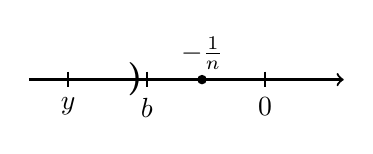
\begin{tikzpicture}[scale=1]
                \draw[thick, ->] (-3,0) -- (1,0);
                \draw[thick] (-2.5,0.1) -- (-2.5,-0.1) node[below] {\(y\)};
                \draw[thick] (-1.5,0.1) -- (-1.5,-0.1) node[below] {\(b\)};
                \node at (-1.65, 0) [scale=1.2] {\textbf{)}};
                \draw[thick] (0,0.1) -- (0,-0.1) node[below] {$0$};
                \filldraw (-0.8,0) circle (1.5pt) node[above] {\(-\frac{1}{n}\)};
            \end{tikzpicture}
            \end{center}
            \(\forall n \ge n_0, \quad b < - \frac{1}{n_0} \le - \frac{1}{n} < 0\). A partir de un \(n_0\) no hay ninguno.
            \[
                \Rightarrow \forall n \ge n_0, \quad -\frac{1}{n} \notin [a, b).
            \]
        \end{itemize}
        No puede ser límite \(\Rightarrow \{-\frac{1}{n}\}_{n \in \mathbb{N}}\) no tiene límite en este espacio topológico.
        
        \item \((\mathbb{R}, \mc T = \{ (-n, n) : n \in \mathbb{N} \} \cup \{ \emptyset, X \})\):
        \[
             \left\{\frac{1}{n}\right\}_{n \in \mathbb{N}} \longrightarrow
            \begin{cases}
                0 & (\text{todos los abiertos contienen al } 0) \\
                \frac{1}{2} & \\
                \lambda \in \mathbb{R} & (\text{converge a cualquier } \lambda \in (-n, n))
            \end{cases}
            \Rightarrow \text{tiene infinitos límites.}
        \]
        \[
            (-n, n) \quad \forall n \in \mathbb{N} \quad \text{y} \quad  \left\{\frac{1}{n}\right\}_{n \ge 1},
        \]
        \[
            (-n, n) \cap  \left\{\frac{1}{n}\right\}_{n \in \mathbb{N}} =  \left\{\frac{1}{n}\right\}_{n \ge 2}.
        \]
    \end{enumerate}
\end{ejem}

\begin{prop}
    Si la sucesión \(\{x_n\}_{n \in \mathbb{N}}\) \textbf{no constante} tiene por límite el punto \(y \in X\), entonces para cualquier subconjunto \(A \subseteq X\) tal que \(\{x_n\}_{n \in \mathbb{N}} \subseteq A\), se verifica que \(y\) es punto de acumulación de \(A\).
\end{prop}

\begin{dem}
    Para todo abierto \(U_y\), \((U_y \cap A) \setminus \{y\} \ne \emptyset\).
    
    Como \(y\) es límite, \(\exists n_0 \in \mathbb{N}\) tal que \(\forall n \ge n_0\),
    \[
        x_n \in U_y \Rightarrow \underbrace{x_n}_{\in A} \in U_y \cap A \Rightarrow x_n \in U_y \cap A \quad \text{con } x_n \ne y.
    \]
\end{dem}

\begin{obs}
    El recíproco en general es falso.
\end{obs}

\section{Condiciones o axiomas de separaci\'on}
Sea $X$ un espacio topol\'ogico. 
\begin{defi} Se tienen las siguientes definiciones de condiciones de separaci\'on 
    \begin{itemize}
        \item Un espacio topol\'ogico $X$ es \textbf{$T_0$} (o \textbf{de Kolmogorov}) si para cualesquiera puntos distintos $x\neq x' \in X$ existe un abierto $U_x$ con $x\in U_x$ y $x'\nin U_x$ \underline{o} existe un abierto $U_{x'}$ con $x'\in U_{x'}$ y $x\nin U_{x'}$.
        \item Un espacio topol\'ogico $X$ es \textbf{$T_1$} (o \textbf{de Fréchet}) si para cualesquiera puntos distintos $x\neq x' \in X$ existe un abierto $U_x$ con $x\in U_x$ y $x'\nin U_x$ \underline{y} existe un abierto $U_{x'}$ con $x'\in U_{x'}$ y $x\nin U_{x'}$. 
        \item Un espacio topol\'ogico $X$ es \textbf{$T_2$} (o \textbf{separado} o \textbf{de Hausdorff}) si para cualesquiera puntos distintos $x\neq x' \in X$ existe un abierto $U_x$ con $x\in U_x$ y existe un abierto $U_{x'}$ con $x'\in U_{x'}$ tal que $U_x\cap U_{x'} = \emptyset$. 
        \item Un espacio topol\'ogico $X$ es \textbf{regular} si para cualequier punto $x \in X$ y cualquier cerrado $C\subset X$ con $x\nin C$ existen abiertos $U_x$ y $U_C$ con $x\in U_x$ y $C\subset U_C$ tal que $U_x\cap U_{C} = \emptyset$.
        \item Un espacio topol\'ogico $X$ es \textbf{$T_3$} si es regular y $T_1$ (los puntos son cerrados). 
        \item Un espacio topol\'ogico $X$ es \textbf{normal} si para cualesquiera cerrados $C$ y $C'$ con \\ $C\cap C'=\emptyset$ existen abiertos con $C \subset U_C, \, C'\subset U_{C'}$ tal que $U_C \cap U_{C'}=\emptyset$. 
        \item Un espacio topol\'ogico $X$ es \textbf{$T_4$} si es normal y $T_1$.  
    \end{itemize}
\end{defi}
\begin{obs}
    $T_4  \Rightarrow T_3 \Rightarrow T_2 \Rightarrow T_1 \Rightarrow T_0$.

    Regular $\Rightarrow T_2 \, \iff \{x\}$ es cerrado para todo $x\in X$. 
\end{obs}
\begin{prop}
    Un espacio topol\'ogico $X$ es $T_0$ $\iff$ se verifica que para cualesquiera puntos $x,x' \in X$, $x\neq x' \iff \overline{\{x\}} \neq \overline{\{x'\}} $. 
\end{prop}
\begin{dem}
$\Rightarrow) $ Es trivial que $\overline{\{x\}}\neq \overline{\{x'\}} \Rightarrow x\neq x'$. 

Veamos que $x\neq x' \Rightarrow \overline{\{x\}} \neq \overline{\{x'\}}$. Sean $x\neq x'$, como el espacio es $T_0$ 
$$\begin{cases}
\text{existe } U_x \ni x \text{ con } x' \nin U_x \\  \qquad \text{\'o} \\  \text{existe } U_{x'} \text{ con } x \nin U_{x'} 
\end{cases}\Rightarrow \begin{cases}
U_{x} \cap \overline{\{x'\}} = \emptyset  \\ \qquad  \text{\'o} \\  U_{x'} \cap \overline{\{x\}} = \emptyset 
\end{cases} \Rightarrow \begin{cases}
x \nin \overline{\{x'\}} \ni x'  \\ \qquad  \text{\'o} \\  x' \nin \overline{\{x\}} \ni x
\end{cases} \Rightarrow \overline{\{x\}} \neq  \overline{\{x'\}}$$
$\Leftarrow) $ Sea $x\neq x'\in X$, como $\overline{\{x\}} \neq \overline{\{x'\}}$ por hip\'otesis, 
$$\Rightarrow \begin{cases}
    x\nin \overline{\{x'\}} \\ \qquad  \text{ \'o } \\ x' \nin \overline{\{x\}} 
\end{cases} \Rightarrow \begin{cases}
    \exists \, U_x \text{ con } U_x \cap \{x'\} =\emptyset \iff x'\nin U_x \\ 
    \qquad \text{ \'o} \\
    \exists \, U_{x'} \text{ con } U_{x'} \cap \{x\} =\emptyset \iff x \nin U_{x'}
\end{cases}$$

$\Leftarrow)$ Sean $x \ne x' \in X$. Como $\overline{\{x\}} \ne \overline{\{x'\}}$ por hipótesis, $\implies x \notin \overline{\{x'\}}$ o $x' \notin \overline{\{x\}}$.
    \begin{align*}
        \implies & \exists U_x \text{ abierto con } U_x \cap \{x'\} = \emptyset \iff x' \notin U_x \\
        & \exists U_{x'} \text{ abierto con } U_{x'} \cap \{x\} = \emptyset \iff x \notin U_{x'}
    \end{align*}
    $\implies$ Es $T_0$.
\end{dem}
\begin{prop}
    Un espacio topol\'ogico es $T_1 \, \iff $ todos los puntos de $X$ son cerrados (dicho de otra forma, $\mc T_{cof} \subset \mc T_X$). 
\end{prop}
\begin{dem}
$\Leftarrow) $ Sean $x\neq x'$, $U_x = X- \{x'\}$ y $U_{x'} = X - \{x\}$ son abiertos por ser complementarios de cerrados y $x\in U_x$ pero $x'\nin U_x$, y $x'\in U_{x'}$ pero $x\nin U_{x'}$, que es la condici\'on de $T_1$.

$\Rightarrow)$ Sea $x\in X$ veamos que $\{x\}$ es cerrado. Supongamos que no, entonces $\{x\} \neq \overline{\{x\}}$ con $x'\in \overline{\{x\}}$ y $x\neq x'$, si fuera $T_1$ existe un abierto $U_{x'}$ con $x'\in U_{x'}$, $U_{x'}\cap \{x\} \neq \emptyset$ por propiedades del cierre, por lo que $x \in U_{x'}$ y no ser\'ia $T_1$, llegando a contradicci\'on. Por lo que $\{x\}$ es cerrado. 
\end{dem}

% ==========================================
% PÁGINA 1
% ==========================================
 

\begin{prop}
    Un espacio topológico $X$ es $T_1 \iff$ todos los puntos de $X$ son cerrados.
\end{prop}

\begin{dem} $\Leftarrow)$ Sean $x \ne x'$.
        \[
            \text{Considero } 
            \begin{aligned}
                U_x &= X \setminus \{x'\} \ni x \\
                U_{x'} &= X \setminus \{x\} \ni x'
            \end{aligned}
            \quad \text{(abiertos)} \implies \text{Es } T_1.
        \]
        \begin{flushright}
            \footnotesize
            $\rightarrow$ Todos los subconjuntos finitos de puntos son cerrados (uniones finitas de cerrados). \\
            $T_1 \iff \mc T_{cof} \subset \mc T_X$.
        \end{flushright}

        $\Rightarrow)$ Sea $x \in X$. Queremos ver que $\{x\}$ es cerrado.
        
        Supongamos que $\{x\}$ no es cerrado $\iff \{x\} \ne \overline{\{x\}} \implies$ existe $x' \in \overline{\{x\}}$ con $x' \ne x$. Por tanto, 
        \[
            \forall \, U_{x'} \text{ abierto con } x' \in U_{x'}, \quad U_{x'} \cap \{x\} \ne \emptyset \implies x \in U_{x'} \implies \bot \quad (\forall \text{ abierto}).
        \]
\end{dem}

\begin{prop}
    $X$ es $T_2 \iff$ dados $x, x' \in X$ con $x \ne x'$, entonces existe un entorno cerrado $V_x$ con $x \in V_x \not\ni x'$ y viceversa, existe un entorno cerrado $V_{x'}$ con $x' \in V_{x'} \not\ni x$.
\end{prop}

\begin{dem} \, 
    
    $\Rightarrow)$ Sean $x \ne x' \in X$. Por ser $X$ $T_2$, existen abiertos $U_x, U_{x'}$ con $U_x \cap U_{x'} = \emptyset \implies U_x \subseteq \underbrace{X \setminus U_{x'}}_{\text{(Cerrado)}}$. Como $X \setminus U_{x'}$ es cerrado, entonces $x \in U_x \subseteq \underbrace{\overline{U}_x}_{V_x} \subseteq X \setminus U_{x'}$, y concluimos.
\end{dem}

\begin{obs}
    Si $V_x$ es entorno cerrado de $x$, entonces existe un abierto $U_x$ con $$x \in U_x \subseteq \underbrace{\overline{U}_x}_{\substack{\text{entorno} \\ \text{cerrado}}} \subseteq \underbrace{V_x}_{\substack{\text{entorno} \\ \text{cerrado}}}$$
\end{obs}

\begin{dem}[Continuación Prop.] \, 

        $\Leftarrow)$ Sean $x \ne x' \in X$. Por hipótesis, existen cerrados $V_x, V_{x'}$ tal que $x \notin V_{x'}, \, x' \notin V_x$.
        
        Entonces, existe un abierto $U_x$ tal que $x \in U_x \subseteq V_x$.
        
        Sea $U_{x'} = X \setminus V_x$, que es abierto, y $x' \in X \setminus V_x$.
        
        Tenemos que $U_x \cap U_{x'} = \emptyset \implies X$ es $T_2$.
\end{dem}

\begin{prop}
    Si $X$ es $T_2$, si una sucesión de puntos $\{x_n\}_{n \in \mathbb{N}} \subseteq X$ tiene límite, este límite es único.
\end{prop}

\begin{dem}
    Supongamos que la sucesión tiene dos límites, $\lim \{x_n\} = x, \, x'$ y que $x \ne x'$. Por ser $T_2$, existen abiertos $U_x, U_{x'}$ tales que $U_x \cap U_{x'} = \emptyset$.
    
% ==========================================
% PÁGINA 2 (pág. 11)
% ==========================================
    \begin{align*}
        \lim \{x_n\} = x \text{ y } x \in U_x &\implies \exists n_0(U_x) \text{ tal que } \forall n \ge n_0, \, x_n \in U_x. \\
        \lim \{x_n\} = x' \text{ y } x' \in U_{x'} &\implies \exists n_0'(U_{x'}) \text{ tal que } \forall n \ge n_0', \, x_n \in U_{x'}.
    \end{align*}
    Sea $N_0 = \max\{n_0, n_0'\}$.
    \[
        \forall n \ge N_0 \implies 
        \begin{cases} 
            \ge n_0 \implies x_n \in U_x \\ 
            \ge n_0' \implies x_n \in U_{x'} 
        \end{cases} 
        \implies x_n \in U_x \cap U_{x'} \ne \emptyset, \quad \forall n \ge N_0 \implies \bot.
    \]
    \end{dem}
\begin{prop}
    $X$ es regular $\iff$ para todo $x \in X$ y todo abierto $U_x$ con $x \in U_x$, existe un entorno (abierto) $V_x$ de $x$ tal que $x \in V_x \subseteq \overline{V}_x \subseteq U_x$.\vspace{-0.3cm}
    \[\vspace{-0.4cm}
        \Updownarrow
    \]
    \begin{center}
        \small Los entornos cerrados de un punto forman base de entornos del punto.
    \end{center}
    Es decir, los entornos cerrados forman base $\iff X$ es regular.
\end{prop}

\begin{dem} $\Rightarrow) $ Sea $x \in X$ y $U_x$ abierto.
        
        $x \notin X \setminus U_x := C$ cerrado. Por ser $X$ regular, existen abiertos $V_x \ni x, \, V_C \supset C$ tales que $V_x \cap V_C = \emptyset$.
        
        Esto implica que $V_x \subseteq X \setminus V_C \subseteq X \setminus C = U_x \implies x \in V_x \subseteq \overline{V}_x \subseteq X \setminus V_C \subseteq U_x$.

        $\Leftarrow)$ Sea $x \in X, \, C \subseteq X$ cerrado con $x \notin C \implies x \in X \setminus C := U_x$ abierto.
        
        Por hipótesis, existe $V_x$ abierto con $x \in V_x \subseteq \overline{V}_x \subseteq U_x$.
        
        Luego $x \in V_x$ y $X \setminus U_x \subseteq \underbrace{X \setminus \overline{V}_x}_{V_C \text{ abierto}}$, con $C = X \setminus U_x$, y $V_x \cap V_C = \emptyset$ porque $V_x \subseteq \overline{V}_x \implies X \setminus \overline{V}_x = V_C$.
\end{dem}

\begin{prop}
    $X$ es normal $\iff$ para todo cerrado $C$ y todo abierto $U_C$ con $C \subseteq U_C$, existe un abierto $V_C$ tal que $C \subseteq V_C \subseteq \overline{V}_C \subseteq U_C$.
    
    Entonces, entornos cerrados de un cerrado son base de entornos de cerrados.
\end{prop}

\begin{dem}
    (Ejercicio).
\end{dem}

\begin{ejem}
    \hfill
    \begin{itemize}
        \item $(X, \mc T_{\text{trivial}})$ no verifica $T_0$, luego no verifica ninguna condición de separación.
        \item $(X, \mc T_{\text{dis}})$ verifica todas.
        \item $(X = \{0, 1\}, \mc T = \{\emptyset, X, \{1\}\})$ es $T_0$ (puedo separar el $1$), pero \textbf{no} $T_1$ (los puntos no son cerrados, el cero sí y el uno no) $\rightarrow \text{Existe } \{1\} \text{ abierto tal que } 1 \in \{1\}, \, 0 \notin \{1\}$.
        \item $(\mathbb{R}^n, \mc T_d)$ es $T_4$ (probar).
    \end{itemize}
\end{ejem}





























































































\begin{comment}
\section{Subespacios topológicos (Topología relativa)}

\begin{defi}
Sea \((X, \mc T_X)\) un espacio topológico y sea \(Y \subseteq X\) un subconjunto. La \textbf{topología inducida} (o relativa) en \(Y\) por \(X\), denotada por \(\mc T_{|Y}\), es:
\[
    \mc T_{|Y} := \{U \cap Y \mid U \in \mc T\} \subseteq \mathcal{P}(Y) \text{}.
\]
El par \((Y, \mc T_{|Y})\) se denomina \textbf{subespacio topológico} de \((X, \mc T)\).
\end{defi}

\begin{prop}
\(\mc T_{|Y}\) es una topología en \(Y\).
\end{prop}

\begin{dem}
\begin{enumerate}
    \item[\textbf{1)}] \(\emptyset = \emptyset \cap Y \in \mc T_{|Y}\) (pues \(\emptyset \in \mc T\)) e \(Y = X \cap Y \in \mc T_{|Y}\) (pues \(X \in \mc T\)).
    \item[\textbf{2)}] Sean \(W_1, \ldots, W_n \in \mc T_{|Y}\). Para cada \(k\), existe \(U_k \in \mc T\) tal que \(W_k = U_k \cap Y\). Entonces:
    \[
        W_1 \cap \ldots \cap W_n = (U_1 \cap Y) \cap \ldots \cap (U_n \cap Y) = (U_1 \cap \ldots \cap U_n) \cap Y \text{}.
    \]
    Como \(U_1 \cap \ldots \cap U_n \in \mc T\), se deduce que \(W_1 \cap \ldots \cap W_n \in \mc T_{|Y}\).
    \item[\textbf{3)}] Sea \(\{W_i\}_{i \in I} \subseteq \mc T_{|Y}\). Para cada \(i \in I\), existe \(U_i \in \mc T\) con \(W_i = U_i \cap Y\). Por distributividad:
    \[
        \bigcup_{i \in I} W_i = \bigcup_{i \in I} (U_i \cap Y) = \left(\bigcup_{i \in I} U_i\right) \cap Y \text{}.
    \]
    Como \(\bigcup_{i \in I} U_i \in \mc T\), su intersección con \(Y\) pertenece a \(\mc T_{|Y}\).
\end{enumerate}
\end{dem}

\begin{obs}
\begin{itemize}
    \item Un abierto \(W \in \mc T_{|Y}\) no tiene por qué ser abierto en \((X, \mc T)\).
    \item Si \(Y \in \mc T\) (es decir, \(Y\) es un subconjunto abierto de \(X\)), entonces todo abierto relativo de \(Y\) es abierto en \(X\), y \(\mc T_{|Y} \subseteq \mc T\).
\end{itemize}
\end{obs}

\begin{ejem}
En \((\mathbb{R}, \mc T_d)\), consideremos \(Y = [1, 2) \cup \{3\} \subset \mathbb{R}\):
\begin{itemize}
    \item \([1, 2) = (0, 2) \cap Y\), con \((0, 2) \in \mc T_d\). Por tanto, \([1, 2)\) es abierto en \((Y, \mc T_{|Y})\), aunque no es abierto en \((\mathbb{R}, \mc T_d)\).
    \item \(\{3\} = (2, 4) \cap Y\), con \((2, 4) \in \mc T_d\). Por tanto, \(\{3\}\) es un abierto en \((Y, \mc T_{|Y})\).
\end{itemize}
\end{ejem}

\section{Topología por entornos}


\begin{teo}
Sea \(X\) un conjunto y sea \(\{\mathcal{E}'(x)\}_{x \in X}\) una familia de subconjuntos de \(X\) asignada a cada punto \(x \in X\) que satisface los axiomas 1, 2, 3 y 4 anteriores. Entonces existe una \textbf{única} topología \(\mc T'\) en \(X\) tal que \(\mathcal{E}_{\mc T'}(x) = \mathcal{E}'(x)\) para todo \(x \in X\).
\end{teo}

\begin{dem}
Definimos la familia:
\[
    \mc T' := \{U \subseteq X \mid \forall x \in U, \; U \in \mathcal{E}'(x)\} \text{}.
\]
\begin{itemize}
    \item[\textbf{a)}] \(\mc T'\) es topología:
    \begin{itemize}
        \item \(\emptyset \in \mc T'\) por vacuidad. Para todo \(x \in X\), por el axioma 1 tenemos \(x \in V\) para cualquier \(V \in \mathcal{E}'(x)\), y como \(V \subseteq X\), por el axioma 3 se tiene \(X \in \mathcal{E}'(x)\), luego \(X \in \mc T'\).
        \item Si \(U_1, U_2 \in \mc T'\) y \(x \in U_1 \cap U_2\), entonces \(U_1 \in \mathcal{E}'(x)\) y \(U_2 \in \mathcal{E}'(x)\). Por el axioma 2, \(U_1 \cap U_2 \in \mathcal{E}'(x)\), luego \(U_1 \cap U_2 \in \mc T'\).
        \item Si \(\{U_i\}_{i \in I} \subseteq \mc T'\) y \(x \in \bigcup_{i \in I} U_i\), existe \(j \in I\) con \(x \in U_j\), luego \(U_j \in \mathcal{E}'(x)\). Al ser \(U_j \subseteq \bigcup U_i\), por el axioma 3 se tiene \(\bigcup U_i \in \mathcal{E}'(x)\), luego \(\bigcup U_i \in \mc T'\).
    \end{itemize}
    \item[\textbf{b)}] Coincidencia de entornos:
    \begin{itemize}
        \item Si \(V \in \mathcal{E}_{\mc T'}(x)\), existe \(U \in \mc T'\) con \(x \in U \subseteq V\). Por definición de \(\mc T'\), \(U \in \mathcal{E}'(x)\), y por el axioma 3, \(V \in \mathcal{E}'(x)\).
        \item Si \(V' \in \mathcal{E}'(x)\), definimos \(U := \{y \in X \mid V' \in \mathcal{E}'(y)\}\). Por el axioma 1, \(y \in U \Rightarrow y \in V'\), luego \(U \subseteq V'\). Veamos que \(U \in \mc T'\): si \(y \in U\), entonces \(V' \in \mathcal{E}'(y)\); por el axioma 4, existe \(W \in \mathcal{E}'(y)\) tal que para todo \(z \in W\) se cumple \(V' \in \mathcal{E}'(z)\) (lo que significa \(W \subseteq U\)), luego por el axioma 3, \(U \in \mathcal{E}'(y)\). Por tanto, \(U \in \mc T'\). Como \(x \in U \subseteq V'\), deducimos que \(V' \in \mathcal{E}_{\mc T'}(x)\).
    \end{itemize}
    \item[\textbf{c)}] Unicidad: si \(\mc T''\) tuviera los mismos entornos, un subconjunto sería abierto si y solo si es entorno de todos sus puntos, lo que forzaría \(\mc T'' = \mc T'\).
\end{itemize}
\end{dem}

\subsection{Bases de entornos (Sistemas fundamentales de entornos)}

\begin{defi}
Sea \((X, \mc T)\) un espacio topológico y \(x \in X\). Una subfamilia \(\mathcal{B}(x) \subseteq \mathcal{E}(x)\) es una \textbf{base de entornos} de \(x\) si para todo entorno \(V \in \mathcal{E}(x)\) existe \(B_x \in \mathcal{B}(x)\) tal que:
\[
    x \in B_x \subseteq V \text{}.
\]
\end{defi}

\begin{prop}
Si \(\{\mathcal{B}(x)\}_{x \in X}\) es una base de entornos para cada \(x \in X\), entonces verifica:
\begin{enumerate}
    \item[\textbf{1)}] \(\forall B \in \mathcal{B}(x)\), \(x \in B\).
    \item[\textbf{2)}] \(\forall B_1, B_2 \in \mathcal{B}(x)\), existe \(B_0 \in \mathcal{B}(x)\) tal que \(B_0 \subseteq B_1 \cap B_2\).
    \item[\textbf{3)}] \(\forall B \in \mathcal{B}(x)\), existe \(B_x \in \mathcal{B}(x)\) tal que para todo \(y \in B_x\) existe \(B_y \in \mathcal{B}(y)\) con \(B_y \subseteq B\).
\end{enumerate}
\end{prop}

\begin{dem}
\begin{enumerate}
    \item[\textbf{1)}] Como \(\mathcal{B}(x) \subseteq \mathcal{E}(x)\), todo \(B \in \mathcal{B}(x)\) es entorno de \(x\), luego \(x \in B\).
    \item[\textbf{2)}] Sean \(B_1, B_2 \in \mathcal{B}(x) \subseteq \mathcal{E}(x)\). Su intersección \(B_1 \cap B_2 \in \mathcal{E}(x)\). Como \(\mathcal{B}(x)\) es base de entornos, existe \(B_0 \in \mathcal{B}(x)\) con \(B_0 \subseteq B_1 \cap B_2\).
    \item[\textbf{3)}] Sea \(B \in \mathcal{B}(x) \subseteq \mathcal{E}(x)\). Por el axioma 4 de entornos, existe \(W \in \mathcal{E}(x)\) tal que para todo \(y \in W\) se tiene \(B \in \mathcal{E}(y)\). Como \(\mathcal{B}(x)\) es base de entornos, existe \(B_x \in \mathcal{B}(x)\) con \(B_x \subseteq W\). Entonces para todo \(y \in B_x \subseteq W\), se cumple \(B \in \mathcal{E}(y)\); como \(\mathcal{B}(y)\) es base de entornos, existe \(B_y \in \mathcal{B}(y)\) tal que \(B_y \subseteq B\).
\end{enumerate}
\end{dem}

\begin{teo}
Dada una familia \(\{\mathcal{B}(x)\}_{x \in X}\) de subconjuntos de \(X\) que satisface las tres propiedades anteriores, existe una única topología en \(X\) de la cual \(\{\mathcal{B}(x)\}\) son bases de entornos.
\end{teo}

\begin{dem}
Definimos para cada \(x \in X\):
\[
    \mathcal{E}(x) := \{V \subseteq X \mid \exists B_x \in \mathcal{B}(x) \text{ tal que } x \in B_x \subseteq V\} \text{}.
\]
Comprobamos que \(\mathcal{E}(x)\) verifica los 4 axiomas del Teorema 5.2:
\begin{enumerate}
    \item[\textbf{1)}] Si \(V \in \mathcal{E}(x)\), existe \(B_x \in \mathcal{B}(x)\) con \(x \in B_x \subseteq V\). Por la propiedad 1, \(x \in B_x\), luego \(x \in V\).
    \item[\textbf{2)}] Si \(V_1, V_2 \in \mathcal{E}(x)\), existen \(B_1, B_2 \in \mathcal{B}(x)\) con \(B_1 \subseteq V_1\) y \(B_2 \subseteq V_2\). Por la propiedad 2, existe \(B_0 \in \mathcal{B}(x)\) con \(B_0 \subseteq B_1 \cap B_2 \subseteq V_1 \cap V_2\), luego \(V_1 \cap V_2 \in \mathcal{E}(x)\).
    \item[\textbf{3)}] Si \(V \in \mathcal{E}(x)\) y \(V \subseteq W\), existe \(B_x \in \mathcal{B}(x)\) con \(B_x \subseteq V \subseteq W\), luego \(W \in \mathcal{E}(x)\).
    \item[\textbf{4)}] Si \(V \in \mathcal{E}(x)\), existe \(B \in \mathcal{B}(x)\) con \(B \subseteq V\). Por la propiedad 3, existe \(B_x \in \mathcal{B}(x)\) tal que para todo \(y \in B_x\) existe \(B_y \in \mathcal{B}(y)\) con \(B_y \subseteq B \subseteq V\). Tomamos \(W := B_x \in \mathcal{B}(x) \subseteq \mathcal{E}(x)\). Para todo \(y \in W\), como \(B_y \subseteq V\), se sigue que \(V \in \mathcal{E}(y)\).
\end{enumerate}
Por el Teorema 5.2, existe una única topología inducida que tiene a \(\mathcal{E}(x)\) como entornos y a \(\mathcal{B}(x)\) como bases de entornos.
\end{dem}

\begin{ejem}
En \((\mathbb{R}^n, d)\) con la distancia euclídea usual:
\begin{itemize}
    \item \(\mathcal{B}(x) = \{B_d(x, \varepsilon) \mid \varepsilon > 0\}\) es una base de entornos de \(x\).
    \item \(\mathcal{B}'(x) = \{B_d(x, \nicefrac{1}{n}) \mid n \in \mathbb{N}\}\) es una base numerable de entornos de \(x\).
    \item \(\overline{\mathcal{B}}(x) = \{\overline{B_d}(x, \nicefrac{1}{n}) \mid n \in \mathbb{N}\}\) (bolas cerradas) también forma una base de entornos, puesto que \(\overline{B_d}(x, \nicefrac{1}{2n}) \subseteq B_d(x, \nicefrac{1}{n})\).
\end{itemize}
\end{ejem}











\chapter{Elementos de un espacio topológico}
Sea $X$ un espacio topológico e $Y \subseteq X$ un subconjunto.

\section{Interior, cierre y puntos especiales}


\begin{defi}
El conjunto de los \textbf{puntos de acumulación} de $Y$ (o conjunto derivado), denotado por $Y'$, es:
\[
    Y' := \{x \in X \mid \forall U_x \text{ abierto con } x \in U_x, \; (U_x \setminus \{x\}) \cap Y \ne \emptyset\}.
\]
Se verifica que:
\[
    \overline{Y} = Y \cup Y'.
\]
\end{defi}

\begin{dem}
Sea $x \in \overline{Y}$. Para todo entorno abierto $U_x \ni x$, $U_x \cap Y \ne \emptyset$. Pueden darse dos casos:
\begin{enumerate}
    \item Existe algún $U_x$ tal que $U_x \cap Y = \{x\}$, lo cual implica $x \in Y \subseteq Y \cup Y'$.
    \item Para todo $U_x$, $U_x \cap Y \ne \{x\}$, lo cual equivale a $(U_x \setminus \{x\}) \cap Y \ne \emptyset$, luego $x \in Y' \subseteq Y \cup Y'$.
\end{enumerate}
Recíprocamente, como $Y \subseteq \overline{Y}$ e $Y' \subseteq \overline{Y}$, se tiene $Y \cup Y' \subseteq \overline{Y}$.
\end{dem}

\begin{defi}
Los \textbf{puntos aislados} de $Y$ son aquellos puntos de $Y$ que no son de acumulación:
\[
    Y^a := \{y \in Y \mid \exists U_y \subseteq X \text{ abierto con } y \in U_y \text{ tal que } U_y \cap Y = \{y\}\}.
\]
Equivalentemente, $Y^a = \{y \in Y \mid \{y\} \text{ es abierto en } (Y, \mc T_{|Y})\}$. Se verifica que $\overline{Y} = Y^a \sqcup Y'$.
\end{defi}

\begin{ejem}
En $\mathbb{R}^2$ con la topología usual, sea $Y = [1, 3) \times [1, 2) \cup \{(4, 1), (5, 1)\}$:
\begin{itemize}
    \item $Y^\circ = (1, 3) \times (1, 2)$.
    \item $\overline{Y} = [1, 3] \times [1, 2] \cup \{(4, 1), (5, 1)\}$.
    \item $Y' = [1, 3] \times [1, 2]$.
    \item $Y^a = \{(4, 1), (5, 1)\}$.
\end{itemize}
\end{ejem}

\begin{defi}
La \textbf{frontera} de $Y$ se define como:
\[
    \operatorname{Fr}(Y) = \partial(Y) := \overline{Y} \cap \overline{X \setminus Y} = \operatorname{Fr}(X \setminus Y).
\]
\end{defi}

\begin{defi}
El \textbf{borde} de $Y$ es:
\[
    b(Y) := Y \cap \operatorname{Fr}(Y) = Y \cap (\overline{Y} \cap \overline{X \setminus Y}) = Y \cap \overline{X \setminus Y}.
\]
\end{defi}

\begin{defi}
El \textbf{exterior} de $Y$ es el interior de su complementario:
\[
    \operatorname{Ext}(Y) := (X \setminus Y)^\circ.
\]
\end{defi}

\begin{ejem}
En $(\mathbb{R}, \mc T_d)$, sea $Y = [0, 1)$:
\begin{itemize}
    \item $Y^\circ = (0, 1)$, $\overline{Y} = [0, 1]$, $Y' = [0, 1]$, $Y^a = \emptyset$.
    \item $X \setminus Y = (-\infty, 0) \cup [1, \infty)$, $\overline{X \setminus Y} = (-\infty, 0] \cup [1, \infty)$.
    \item $\operatorname{Fr}(Y) = \{0, 1\}$.
    \item $b(Y) = \{0\}$.
    \item $\operatorname{Ext}(Y) = (-\infty, 0) \cup (1, \infty)$.
\end{itemize}
\end{ejem}

\section{Propiedades fundamentales de los operadores}

\begin{propi}
Sean $X$ un espacio topológico e $Y \subseteq X$. Se verifican:
\begin{enumerate}
    \item[\textbf{I.}] $Y^\circ \cap \operatorname{Fr}(Y) = \emptyset$.
    \item[\textbf{II.}] $\operatorname{Ext}(Y) \cap \operatorname{Fr}(Y) = \emptyset$.
    \item[\textbf{III.}] $Y^\circ \cap b(Y) = \emptyset$.
    \item[\textbf{IV.}] $Y = Y^\circ \sqcup b(Y)$.
    \item[\textbf{V.}] $\overline{Y} = Y^\circ \sqcup \operatorname{Fr}(Y)$.
    \item[\textbf{VI.}] $Y$ es abierto $\iff b(Y) = \emptyset$.
    \item[\textbf{VII.}] $Y$ es cerrado $\iff \operatorname{Fr}(Y) \subseteq Y$.
    \item[\textbf{VIII.}] $\operatorname{Ext}(Y) = X \setminus \overline{Y}$.
    \item[\textbf{IX.}] $\overline{X \setminus Y} = X \setminus Y^\circ$.
    \item[\textbf{X.}] $\overline{Y^\circ} \subseteq \overline{Y}$ (en general no se da la igualdad).
    \item[\textbf{XI.}] $Y^\circ \subseteq (\overline{Y})^\circ$ (en general no se da la igualdad).
\end{enumerate}
\end{propi}

\begin{dem}
\begin{itemize}
    \item[\textbf{I.}] $Y^\circ \cap \operatorname{Fr}(Y) = Y^\circ \cap (\overline{Y} \cap \overline{X \setminus Y}) = Y^\circ \cap \overline{X \setminus Y} = \emptyset$, pues si $y \in Y^\circ$, existe un abierto $U_y \subseteq Y$, con lo cual $U_y \cap (X \setminus Y) = \emptyset$, lo que implica $y \notin \overline{X \setminus Y}$.
    \item[\textbf{II.}] $\operatorname{Ext}(Y) \cap \operatorname{Fr}(Y) = (X \setminus Y)^\circ \cap \operatorname{Fr}(X \setminus Y) = \emptyset$ aplicando la propiedad I a $X \setminus Y$.
    \item[\textbf{III.}] $Y^\circ \cap b(Y) = Y^\circ \cap (Y \cap \operatorname{Fr}(Y)) = Y^\circ \cap \operatorname{Fr}(Y) = \emptyset$.
    \item[\textbf{IV.}] Si $y \in Y$, o bien $y \in Y^\circ$, o bien para todo abierto $U \ni y$ se tiene $U \not\subseteq Y$, es decir, $U \cap (X \setminus Y) \ne \emptyset$, lo que implica $y \in \overline{X \setminus Y}$; luego $y \in Y \cap \overline{X \setminus Y} = b(Y)$. La unión es disjunta por III.
    \item[\textbf{V.}] Análoga a IV usando $\overline{Y}$ y $\operatorname{Fr}(Y)$.
    \item[\textbf{VI.}] $Y$ es abierto $\iff Y = Y^\circ \iff b(Y) = Y \setminus Y^\circ = \emptyset$.
    \item[\textbf{VII.}] $Y$ es cerrado $\iff X \setminus Y$ es abierto $\iff b(X \setminus Y) = \emptyset \iff (X \setminus Y) \cap \operatorname{Fr}(Y) = \emptyset \iff \operatorname{Fr}(Y) \subseteq Y$.
    \item[\textbf{VIII.}] $x \in \operatorname{Ext}(Y) \iff x \in (X \setminus Y)^\circ \iff \exists U_x \text{ abierto con } U_x \subseteq X \setminus Y \iff U_x \cap Y = \emptyset \iff x \notin \overline{Y} \iff x \in X \setminus \overline{Y}$.
    \item[\textbf{IX.}] Tomando complementarios en VIII: $\overline{X \setminus Y} = X \setminus (X \setminus (X \setminus Y))^\circ = X \setminus Y^\circ$.
    \item[\textbf{X.}] Como $Y^\circ \subseteq Y \Rightarrow \overline{Y^\circ} \subseteq \overline{Y}$. En $(\mathbb{R}, \mc T_d)$, para $\mathbb{Q}$ se tiene $\mathbb{Q}^\circ = \emptyset \Rightarrow \overline{\mathbb{Q}^\circ} = \emptyset \ne \mathbb{R} = \overline{\mathbb{Q}}$.
    \item[\textbf{XI.}] Como $Y^\circ$ es un abierto contenido en $Y \subseteq \overline{Y}$, necesariamente $Y^\circ \subseteq (\overline{Y})^\circ$. Para $\mathbb{Q}$ en $\mathbb{R}$: $\mathbb{Q}^\circ = \emptyset$, pero $(\overline{\mathbb{Q}})^\circ = \mathbb{R}^\circ = \mathbb{R}$.
\end{itemize}
\end{dem}

\section{Subconjuntos densos y clausura relativa}

\begin{defi}
Sea $X$ un espacio topológico e $Y \subseteq X$. Se dice que $Y$ es \textbf{denso} en $X$ si su cierre es el espacio total:
\[
    \overline{Y} = X.
\]
\end{defi}

\begin{prop}
Un subconjunto $Y \subseteq X$ es denso $\iff$ todo abierto no vacío $U \subseteq X$ corta a $Y$ ($U \cap Y \ne \emptyset$).
\end{prop}

\begin{dem}
($\Rightarrow$) Sea $U \ne \emptyset$ abierto en $X$. Sea $x \in U$. Como $X = \overline{Y}$, $x \in \overline{Y}$, por lo que todo entorno abierto de $x$ corta a $Y$; en particular, $U \cap Y \ne \emptyset$.

($\Leftarrow$) Sea $x \in X$. Todo abierto $U \ni x$ es no vacío, luego corta a $Y$, de donde $x \in \overline{Y}$. Por tanto, $X \subseteq \overline{Y} \Rightarrow \overline{Y} = X$.
\end{dem}

\begin{prop}
Sea $Y \subseteq X$ un subespacio topológico y sea $Z \subseteq Y$. Denotemos por $\overline{Z}^X$ la clausura de $Z$ en $X$. Entonces $Z$ es cerrado en $Y$ si y solo si:
\[
    Z = \overline{Z}^X \cap Y.
\]
\end{prop}

\begin{dem}
Si $Z$ es cerrado en $Y$, existe un cerrado $C \subseteq X$ tal que $Z = C \cap Y$. Como $Z \subseteq C$ y $C$ es cerrado en $X$, $\overline{Z}^X \subseteq C$. Por ende, $Z \subseteq \overline{Z}^X \cap Y \subseteq C \cap Y = Z$, de modo que $Z = \overline{Z}^X \cap Y$. El recíproco es inmediato, ya que $\overline{Z}^X$ es cerrado en $X$.
\end{dem}






























\section{Límites de sucesiones}

\begin{defi}
Sea $X$ un espacio topológico y $\{x_n\}_{n \in \mathbb{N}} \subseteq X$ una sucesión de puntos en $X$ (es decir, una aplicación $x \colon \mathbb{N} \to X$). Se dice que un punto $y \in X$ es \textbf{límite} de la sucesión $\{x_n\}$ (y escribimos $\lim_{n \to \infty} x_n = y$) si para todo entorno $V \in \mathcal{E}(y)$ (o para todo abierto $U \ni y$), existe $n_0(V) \in \mathbb{N}$ tal que:
\[
    \forall n \ge n_0(V), \quad x_n \in V.
\]
\end{defi}

\begin{defi}
Una sucesión $\{x_n\}$ es \textbf{no constante} si para todo $n_0 \in \mathbb{N}$ existe $n > n_0$ tal que $x_n \ne x_{n_0}$. Si una sucesión es constante a partir de un término, existe $n_0$ tal que $\forall n \ge n_0$, $x_n = x_{n_0}$, en cuyo caso $\lim x_n = x_{n_0}$.
\end{defi}

\begin{propi}
Sea $\{x_n\} \subseteq X$ una sucesión no constante tal que $\lim_{n \to \infty} x_n = y$. Si consideramos el conjunto de sus términos $S = \{x_n\}_{n \in \mathbb{N}} \subseteq X$, entonces $y \in S'$. En particular, si $S \subseteq A$, entonces $y \in A'$.
\end{propi}

\begin{dem}
Basta probar que para todo entorno $V \in \mathcal{E}(y)$, $(V \setminus \{y\}) \cap S \ne \emptyset$. Como $\lim x_n = y$, existe $n_0$ tal que $\forall n \ge n_0$, $x_n \in V$. Al ser $\{x_n\}$ no constante, existen términos con $x_n \ne y$, luego $(V \setminus \{y\}) \cap S \ne \emptyset$, concluyendo que $y \in S'$.
\end{dem}

\begin{obs}
El recíproco no es cierto en general (en espacios métricos $(\mathbb{R}^n, \mc T_d)$ sí lo es). Además, en un espacio topológico general, el límite de una sucesión \textbf{no tiene por qué ser único}.
\end{obs}

\begin{ejem}
\begin{itemize}
    \item En $(\mathbb{R}, \mc T = \{\emptyset, \mathbb{R}\} \cup \{(-n, n) \mid n \in \mathbb{N}\})$, consideremos $\{\nicefrac{1}{n}\}$. Se tiene que $\lim_{n \to \infty} \nicefrac{1}{n} = a$ para \textbf{todo} $a \in \mathbb{R}$, ya que dado cualquier abierto no vacío $(-m, m)$, existe $n_0$ a partir del cual $\nicefrac{1}{n} \in (-m, m)$ y todo punto $a$ está en algún $(-m, m)$.
    \item En la recta de Sorgenfrey $(\mathbb{R}, \mc T_{\text{Sorg}})$: para la sucesión $\{-\nicefrac{1}{n}\}$, se tiene que $\lim_{n \to \infty} (-\nicefrac{1}{n})$ no converge a $0$, pues $[0, 1) \cap \{-\nicefrac{1}{n}\} = \emptyset$. En cambio, $\{\nicefrac{1}{n}\}$ sí converge únicamente a $0$.
\end{itemize}
\end{ejem}

\section{Axiomas de separación}

Sea $X$ un espacio topológico:
\begin{itemize}
    \item \textbf{Axioma $T_0$ (de Kolmogorov):} Para cualesquiera $x \ne x' \in X$, existe un abierto $U_x$ con $x \in U_x$ y $x' \notin U_x$, o bien existe un abierto $U_{x'}$ con $x' \in U_{x'}$ y $x \notin U_{x'}$.
    \item \textbf{Axioma $T_1$ (de Fréchet):} Para cualesquiera $x \ne x' \in X$, existe un abierto $U_x$ con $x \in U_x$, $x' \notin U_x$, y existe un abierto $U_{x'}$ con $x' \in U_{x'}$, $x \notin U_{x'}$.
    \item \textbf{Axioma $T_2$ (de Hausdorff o separado):} Para cualesquiera $x \ne x' \in X$, existen abiertos disjuntos $U_x, U_{x'}$ con $x \in U_x$, $x' \in U_{x'}$ y $U_x \cap U_{x'} = \emptyset$.
    \item \textbf{Axioma $T_3$ (regular):} $X$ es $T_1$ y para todo punto $x \in X$ y todo cerrado $C \subseteq X$ con $x \notin C$, existen abiertos disjuntos $U_x, U_C$ tales que $x \in U_x$, $C \subseteq U_C$ y $U_x \cap U_C = \emptyset$.
    \item \textbf{Axioma $T_{3\,1/2}$ (de Tychonoff o completamente regular):} $X$ es $T_1$ y para todo $x \in X$ y todo cerrado $C \subseteq X$ con $x \notin C$, existe una función continua $f \colon X \to [0, 1]$ tal que $f(x) = 0$ y $f(C) = \{1\}$.
    \item \textbf{Axioma $T_4$ (normal):} $X$ es $T_1$ y para cualesquiera cerrados disjuntos $C_1, C_2 \subseteq X$ ($C_1 \cap C_2 = \emptyset$), existen abiertos disjuntos $U_{C_1}, U_{C_2}$ con $C_1 \subseteq U_{C_1}$, $C_2 \subseteq U_{C_2}$ y $U_{C_1} \cap U_{C_2} = \emptyset$.
\end{itemize}

\begin{obs}
Se verifican las implicaciones:
\[
    T_4 \Rightarrow T_{3\,1/2} \Rightarrow T_3 \Rightarrow T_2 \Rightarrow T_1 \Rightarrow T_0.
\]
En un espacio $T_2$, si una sucesión converge, su límite es \textbf{único}.
\end{obs}

\begin{ejem}
\begin{itemize}
    \item $(X, \mc T_{\text{trivial}})$ con $|X| \ge 2$ no verifica ningún axioma de separación.
    \item El espacio de Sierpiński $X = \{a, b\}$ con $\mc T = \{\emptyset, X, \{a\}\}$ es $T_0$, pero no es $T_1$.
    \item $(\mathbb{R}^n, \mc T_d)$ es un espacio $T_4$ (y por tanto cumple todos los axiomas anteriores).
\end{itemize}
\end{ejem}

\subsection*{Caracterizaciones de los axiomas de separación}

\begin{prop}
Un espacio topológico $X$ es $T_0 \iff$ puntos distintos tienen clausuras distintas, es decir:
\[
    x \ne y \Rightarrow \overline{\{x\}} \ne \overline{\{y\}}.
\]
\end{prop}

\begin{dem}
($\Rightarrow$) Supongamos que $\overline{\{x\}} = \overline{\{y\}}$. Como $x \in \overline{\{x\}} = \overline{\{y\}}$, todo abierto que contiene a $x$ corta a $\{y\}$, es decir, contiene a $y$. Análogamente, todo abierto que contiene a $y$ contiene a $x$. Por tanto, no puede existir un abierto que contenga a uno sin contener al otro, contradiciendo que $X$ es $T_0$.

($\Leftarrow$) Si $x \ne y$ y $\overline{\{x\}} \ne \overline{\{y\}}$, existe sin pérdida de generalidad un punto $z \in \overline{\{x\}} \setminus \overline{\{y\}}$. Como $z \notin \overline{\{y\}}$, existe un abierto $U$ con $z \in U$ tal que $U \cap \{y\} = \emptyset$, luego $y \notin U$. Como $z \in \overline{\{x\}}$, $U \cap \{x\} \ne \emptyset \Rightarrow x \in U$. Así, $U$ contiene a $x$ pero no a $y$, concluyendo que $X$ es $T_0$.
\end{dem}

\begin{prop}
Un espacio topológico $X$ es $T_1 \iff$ todos los conjuntos unitarios $\{x\}$ son cerrados ($\overline{\{x\}} = \{x\}$ para todo $x \in X$).
\end{prop}

\begin{dem}
($\Rightarrow$) Para todo $y \ne x$, por ser $T_1$ existe un abierto $U_y$ con $y \in U_y$ y $x \notin U_y$. Entonces $X \setminus \{x\} = \bigcup_{y \ne x} U_y$ es unión de abiertos, luego es abierto, y $\{x\}$ es cerrado.

($\Leftarrow$) Si los puntos son cerrados, para $x \ne y$, $U_x = X \setminus \{y\}$ es un abierto con $x \in U_x$, $y \notin U_x$, y $U_y = X \setminus \{x\}$ es un abierto con $y \in U_y$, $x \notin U_y$. Por tanto, $X$ es $T_1$.
\end{dem}

\begin{prop}
Un espacio topológico $X$ es $T_2 \iff$ para cualesquiera $x \ne y \in X$, existen abiertos $U_x, U_y$ tales que:
\[
    \overline{U}_x \cap U_y = \emptyset.
\]
\end{prop}

\begin{dem}
($\Rightarrow$) Si $X$ es $T_2$, existen abiertos disjuntos $U_x, V$ con $x \in U_x$, $y \in V$. Como $U_x \subseteq X \setminus V$ y $X \setminus V$ es cerrado, $\overline{U}_x \subseteq X \setminus V$, de donde $\overline{U}_x \cap V = \emptyset$. Tomando $U_y = V$ se tiene el resultado.

($\Leftarrow$) Si $\overline{U}_x \cap U_y = \emptyset$, como $U_x \subseteq \overline{U}_x$, se deduce $U_x \cap U_y = \emptyset$, luego $X$ es $T_2$.
\end{dem}

\begin{prop}
Un espacio $T_1$ es $T_3 \iff$ para todo punto $x \in X$ y todo abierto $U \ni x$, existe un abierto $V$ tal que:
\[
    x \in V \subseteq \overline{V} \subseteq U.
\]
\end{prop}

\begin{dem}
($\Rightarrow$) Sea $x \in U$ abierto. El conjunto $C = X \setminus U$ es cerrado y $x \notin C$. Por ser $T_3$, existen abiertos disjuntos $V_x, V_C$ con $x \in V_x$ y $C \subseteq V_C$. Como $V_x \cap V_C = \emptyset$, $V_x \subseteq X \setminus V_C \Rightarrow \overline{V}_x \subseteq X \setminus V_C \subseteq X \setminus C = U$.

($\Leftarrow$) Sea $C$ cerrado y $x \notin C$. Entonces $U = X \setminus C$ es un abierto que contiene a $x$. Por hipótesis, existe un abierto $V_1$ con $x \in V_1 \subseteq \overline{V}_1 \subseteq U$. Tomando $V_2 = X \setminus \overline{V}_1$, $V_2$ es abierto, $C = X \setminus U \subseteq V_2$ y $V_1 \cap V_2 = \emptyset$. Luego $X$ es $T_3$.
\end{dem}

\begin{obs}
La proposición anterior equivale a afirmar que en un espacio regular, los entornos cerrados de cada punto forman una base de entornos de dicho punto.
\end{obs}

\begin{prop}
Un espacio $T_1$ es $T_4 \iff$ para todo cerrado $C \subseteq X$ y todo abierto $U$ con $C \subseteq U$, existe un abierto $V$ tal que:
\[
    C \subseteq V \subseteq \overline{V} \subseteq U.
\]
\end{prop}

\begin{dem}
($\Rightarrow$) Si $C \subseteq U$, $C' = X \setminus U$ es cerrado y disjunto con $C$. Por ser $T_4$, existen abiertos disjuntos $V, V'$ con $C \subseteq V$ y $C' \subseteq V'$. Entonces $\overline{V} \subseteq X \setminus V' \subseteq X \setminus C' = U$.

($\Leftarrow$) Si $C_1 \cap C_2 = \emptyset$, $C_1 \subseteq X \setminus C_2 = U$ abierto. Existe un abierto $V$ con $C_1 \subseteq V \subseteq \overline{V} \subseteq U$. Tomando $V_2 = X \setminus \overline{V}$, $V$ y $V_2$ son abiertos disjuntos que separan $C_1$ y $C_2$.
\end{dem}

\begin{defi}
Sea $X$ un espacio topológico y $A \subseteq X$. Un subconjunto $W \subseteq X$ es un \textbf{entorno de $A$} si existe un abierto $V \subseteq X$ tal que $A \subseteq V \subseteq W$.
\end{defi}

\begin{obs}
De forma análoga al caso de puntos, la caracterización de $T_4$ equivale a que los entornos cerrados de un conjunto cerrado forman una base de entornos de dicho cerrado.
\end{obs}

\begin{obs}
En un espacio topológico $X$, todo punto $x \in X$ es un conjunto abierto $\iff X$ tiene la topología discreta.
\end{obs}

























\chapter{Aplicaciones continuas}

\section{Definición de aplicación continua}

\begin{defi}
Sean $(X, \mc T_X)$ e $(Y, \mc T_Y)$ espacios topológicos. Una aplicación $f \colon (X, \mc T_X) \to (Y, \mc T_Y)$ se dice \textbf{continua} si:
\[
    f^*(\mc T_Y) \subseteq \mc T_X.
\]
Es decir, para todo abierto $V \in \mc T_Y$, su anti-imagen es abierta en $X$:
\[
    f^{-1}(V) \in \mc T_X.
\]
Son condiciones equivalentes:
\begin{enumerate}
    \item[\textbf{1)}] $f$ es continua.
    \item[\textbf{2)}] Para todo cerrado $Z \subseteq Y$, su anti-imagen $f^{-1}(Z) \subseteq X$ es un conjunto cerrado en $X$.
    \item[\textbf{3)}] Para todo punto $x \in X$ y para todo entorno $W \in \mathcal{E}(f(x))$, $f^{-1}(W)$ es un entorno de $x$ en $X$ ($f^{-1}(W) \in \mathcal{E}(x)$).
\end{enumerate}
\end{defi}

\begin{prop}
Sea $\mathcal{B}$ una base de la topología $\mc T_Y$ de $Y$. Son equivalentes:
\begin{enumerate}
    \item[\textbf{1)}] $f$ es continua.
    \item[\textbf{2)}] Para todo abierto básico $B \in \mathcal{B}$, $f^{-1}(B)$ es abierto en $X$.
    \item[\textbf{3)}] Para todo cerrado básico $B \in \mathcal{B}_{\text{cerr}}$, $f^{-1}(B)$ es cerrado en $X$.
    \item[\textbf{4)}] Para todo $x \in X$ y todo entorno básico $B \in \mathcal{B}(f(x))$, $f^{-1}(B)$ es entorno de $x$.
\end{enumerate}
\end{prop}

\begin{dem}
\begin{itemize}
    \item[\textbf{1 $\Rightarrow$ 2:}] Inmediato, pues todo abierto básico es un abierto de $Y$.
    \item[\textbf{2 $\Rightarrow$ 1:}] Dado $V \in \mc T_Y$, existe una familia $\{B_i\}_{i \in I} \subseteq \mathcal{B}$ tal que $V = \bigcup_{i \in I} B_i$. Entonces:
    \[
        f^{-1}(V) = f^{-1}\left(\bigcup_{i \in I} B_i\right) = \bigcup_{i \in I} f^{-1}(B_i).
    \]
    Como cada $f^{-1}(B_i)$ es abierto por hipótesis, su unión arbitraria es abierta en $X$. (Como caso límite, $f^{-1}(\emptyset) = \emptyset \in \mc T_X$).
    \item[\textbf{1 $\iff$ 3:}] Si $\mathcal{B}$ es base de cerrados, todo cerrado $Z \subseteq Y$ se escribe como $Z = \bigcap_{i \in I} B_i$. La anti-imagen $f^{-1}(Z) = \bigcap_{i \in I} f^{-1}(B_i)$ es intersección de cerrados, luego cerrada.
    \item[\textbf{1 $\iff$ 4:}] Dado un entorno $W \in \mathcal{E}(f(x))$, existe un entorno básico $B \in \mathcal{B}(f(x))$ tal que $B \subseteq W$. Por tanto, $x \in f^{-1}(B) \subseteq f^{-1}(W)$, con lo cual $f^{-1}(W)$ es entorno de $x$.
\end{itemize}
\end{dem}

\begin{obs}
La continuidad de una función concierne al comportamiento de la anti-imagen $f^* = f^{-1}$ sobre la topología. En general, la imagen directa $f_*(U) = f(U)$ de un abierto $U$ no tiene por qué ser abierta.
\end{obs}

\section{Homeomorfismos}

\begin{defi}
Sean $X, Y$ espacios topológicos. Un \textbf{homeomorfismo} (o isomorfismo topológico) es una aplicación $f \colon X \to Y$ que cumple:
\begin{enumerate}
    \item $f$ es continua.
    \item $f$ es biyectiva.
    \item Su inversa $f^{-1} \colon Y \to X$ es continua.
\end{enumerate}
Dos espacios topológicos se dicen \textbf{homeomorfos} (denotado $X \cong Y$ o $X \simeq Y$) si existe un homeomorfismo entre ellos.
\end{defi}

\begin{ejem}[La aplicación identidad]
Sea $X$ un conjunto:
\begin{itemize}
    \item $\operatorname{Id}_X \colon (X, \mc T_{\text{discreta}}) \to (X, \mc T_{\text{trivial}})$ es continua y biyectiva, pero su inversa $\operatorname{Id}_X^{-1} \colon (X, \mc T_{\text{trivial}}) \to (X, \mc T_{\text{discreta}})$ no es continua (si $|X| \ge 2$). Por tanto, la identidad no siempre es un homeomorfismo si cambian las topologías.
    \item $\operatorname{Id}_X \colon (X, \mc T) \to (X, \mc T)$ es siempre un homeomorfismo.
\end{itemize}
\end{ejem}

\begin{ejem}[Topología trivial y discreta]
\begin{itemize}
    \item Toda aplicación $f \colon (X, \mc T_X) \to (Y, \mc T_{\text{trivial}})$ es continua. Recíprocamente, si para todo espacio $X$ cualquier aplicación $f \colon X \to Y$ es continua, entonces $\mc T_Y = \mc T_{\text{trivial}}$.
    \item Toda aplicación $f \colon (X, \mc T_{\text{discreta}}) \to (Y, \mc T_Y)$ es continua. Recíprocamente, si para todo espacio $Y$ cualquier aplicación $f \colon X \to Y$ es continua, entonces $\mc T_X = \mc T_{\text{discreta}}$.
\end{itemize}
\end{ejem}

\begin{obs}
Si $f \colon (X, \mc T_X) \to (Y, \mc T_Y)$ es continua:
\begin{itemize}
    \item Si afinamos la topología del dominio ($\mc T_X \subseteq \mc T_X'$), $f \colon (X, \mc T_X') \to (Y, \mc T_Y)$ sigue siendo continua.
    \item Si engrosamos la topología del codominio ($\mc T_Y' \subseteq \mc T_Y$), $f \colon (X, \mc T_X) \to (Y, \mc T_Y')$ sigue siendo continua.
\end{itemize}
\end{obs}

\begin{ejem}[Aplicación constante]
Dados $(X, \mc T_X)$, $(Y, \mc T_Y)$ y un punto fijo $y_0 \in Y$, la aplicación constante $f_{y_0} \colon X \to Y$, dada por $f_{y_0}(x) = y_0$, es continua:
\[
    f_{y_0}^{-1}(V) = \begin{cases} \emptyset \in \mc T_X & \text{si } y_0 \notin V, \\ X \in \mc T_X & \text{si } y_0 \in V. \end{cases}
\]
\end{ejem}

\begin{ejem}[Homeomorfismos en la recta real y proyección estereográfica]
En $(\mathbb{R}, \mc T_d)$:
\begin{itemize}
    \item Dados $a < b$, $[a, b] \cong [0, 1]$ mediante la traslación y dilatación $w \mapsto \frac{w - a}{b - a}$.
    \item Del mismo modo, $(a, b) \cong (0, 1) \cong (-1, 1)$.
    \item $(-1, 1) \cong \mathcal{SC}_{(0, 1)}$ (semicircunferencia inferior abierta de centro $(0, 1)$ y radio $1$) proyectando verticalmente: $x \mapsto (x, 1 - \sqrt{1 - x^2})$.
    \item Proyección estereográfica desde el polo superior $(0, 1)$ sobre el eje real $y = 0$: define un homeomorfismo explícito entre la semicircunferencia abierta $\mathcal{SC}_{(0, 1)}$ y toda la recta real $\mathbb{R}$.
\end{itemize}
Por composición de homeomorfismos:
\[
    (a, b) \cong (-1, 1) \cong \mathcal{SC}_{(0, 1)} \cong \mathbb{R}.
\]

\begin{center}
\begin{tikzpicture}[scale=1.5]
    % Eje horizontal y=0
    \draw[->,thick] (-3.5,0) -- (3.5,0) node[right] {$y=0$ ($\mathbb{R}$)};
    \draw[->,thick] (0,-0.3) -- (0,1.5) node[above] {$y$};
    
    % Semicircunferencia inferior centrada en (0,1) de radio 1
    \draw[thick,blue] (1,1) arc (0:-180:1);
    \node[blue] at (1.2,0.4) {$\mathcal{SC}_{(0,1)}$};
    
    % Polo superior
    \filldraw[black] (0,1) circle (1.5pt) node[above] {$(0, 1)$};
    
    % Rayos de proyección estereográfica
    \draw[dashed,teal] (0,1) -- (2.3,0);
    \draw[dashed,teal] (0,1) -- (-2.5,0);
    \draw[dashed,teal] (0,1) -- (0.8,0);
    
    % Puntos en la semicircunferencia y en el eje
    \filldraw[teal] ({cos(-35)},{1+sin(-35)}) circle (1.2pt);
    \filldraw[teal] (2.3,0) circle (1.2pt) node[below] {$t_1$};
    
    \filldraw[teal] ({cos(-140)},{1+sin(-140)}) circle (1.2pt);
    \filldraw[teal] (-2.5,0) circle (1.2pt) node[below] {$t_2$};
    
    \node at (0,-0.5) [align=center] {Proyección estereográfica: $\mathcal{SC}_{(0, 1)} \xrightarrow{\;\sim\;} \mathbb{R}$};
\end{tikzpicture}
\end{center}
Nótese que esto no es aplicable a $[a, b]$, pues la proyección estereográfica no está definida en los extremos de la semicircunferencia cerrada.
\end{ejem}

\section{Propiedades de las aplicaciones continuas}

\begin{propi}[Inclusión natural]
Sea $(X, \mc T_X)$ un espacio topológico y $A \subseteq X$ dotado de la topología inducida $\mc T_{X|A}$. La inclusión canónica:
\[
    i_A \colon (A, \mc T_{X|A}) \longhookrightarrow (X, \mc T_X)
\]
es continua, ya que para todo abierto $U \in \mc T_X$, $i_A^{-1}(U) = U \cap A \in \mc T_{X|A}$.
\end{propi}

\begin{propi}
\begin{enumerate}
    \item[\textbf{1)}] \textbf{Composición:} Si $f \colon X \to Y$ y $g \colon Y \to Z$ son continuas, entonces $g \circ f \colon X \to Z$ es continua.
    \item[\textbf{2)}] \textbf{Restricción del dominio:} Si $f \colon X \to Y$ es continua y $A \subseteq X$, la restricción $f_{|A} \colon (A, \mc T_{X|A}) \to Y$ es continua, dado que $f_{|A} = f \circ i_A$.
    \item[\textbf{3)}] \textbf{Restricción del codominio:} Si $f \colon X \to Y$ es continua y $Z \subseteq Y$ cumple $\operatorname{Im}(f) \subseteq Z$, la aplicación $f^Z \colon X \to (Z, \mc T_{Y|Z})$ es continua.
    \item[\textbf{4)}] \textbf{Extensión del codominio:} Si $f \colon X \to Z$ es continua y $Z \subseteq Y$, entonces $f^Y \colon X \to Y$ (dada por $f^Y = i_Z \circ f$) es continua.
    \item[\textbf{5)}] \textbf{Propiedad local (recubrimiento abierto):} Sea $\{U_i\}_{i \in I}$ un recubrimiento por abiertos de $X$ ($X = \bigcup_{i \in I} U_i$ con $U_i \in \mc T_X$). Una aplicación $f \colon X \to Y$ es continua si y solo si cada restricción $f_{|U_i} \colon U_i \to Y$ es continua para todo $i \in I$.
\end{enumerate}
\end{propi}

\begin{dem}
\begin{itemize}
    \item[\textbf{1)}] Para todo $W \subseteq Z$ abierto, $(g \circ f)^{-1}(W) = f^{-1}(g^{-1}(W))$. Por ser $g$ continua, $g^{-1}(W)$ es abierto en $Y$; por ser $f$ continua, $f^{-1}(g^{-1}(W))$ es abierto en $X$.
    \item[\textbf{2)}] Es consecuencia de 1 por ser $f_{|A} = f \circ i_A$, composición de continuas.
    \item[\textbf{3)}] Si $V' \subseteq Z$ es abierto en $Z$, existe un abierto $V \subseteq Y$ con $V' = V \cap Z$. Entonces $(f^Z)^{-1}(V') = f^{-1}(V \cap Z) = f^{-1}(V) \in \mc T_X$.
    \item[\textbf{4)}] Directo por composición: $f^Y = i_Z \circ f$.
    \item[\textbf{5)}] Sea $V \subseteq Y$ abierto. Entonces:
    \[
        f^{-1}(V) = f^{-1}(V) \cap \left(\bigcup_{i \in I} U_i\right) = \bigcup_{i \in I} (f^{-1}(V) \cap U_i) = \bigcup_{i \in I} (f_{|U_i})^{-1}(V).
    \]
    Como cada $f_{|U_i}$ es continua, $(f_{|U_i})^{-1}(V)$ es abierto en $U_i$. Al ser $U_i$ abierto en $X$, cada término es abierto en $X$, y su unión es abierta en $X$.
\end{itemize}
\end{dem}

\begin{prop}[Continuidad en un punto]
Una aplicación $f \colon (X, \mc T_X) \to (Y, \mc T_Y)$ es continua si y solo si es continua en cada punto $x \in X$, es decir: para todo entorno $V \in \mathcal{E}(f(x))$, $f^{-1}(V) \in \mathcal{E}(x)$. En $(\mathbb{R}, \mc T_d)$, equivale a la definición usual: $\forall \varepsilon > 0$, $\exists \delta > 0$ tal que $|x - x'| < \delta \Rightarrow |f(x) - f(x')| < \varepsilon$.
\end{prop}

\section{Aplicaciones abiertas, cerradas e inmersiones}

\begin{defi}
Sea $f \colon X \to Y$ una aplicación entre espacios topológicos:
\begin{itemize}
    \item $f$ es \textbf{abierta} si para todo abierto $U \in \mc T_X$, la imagen $f(U)$ es abierta en $Y$.
    \item $f$ es \textbf{cerrada} si para todo cerrado $C \subseteq X$, la imagen $f(C)$ es cerrada en $Y$.
\end{itemize}
\end{defi}

\begin{obs}
Una aplicación continua puede no ser abierta ni cerrada:
\begin{itemize}
    \item Sea $f \colon (\mathbb{R}, \mc T_d) \to (\mathbb{R}, \mc T_d)$ dada por $f(x) = x^2$. Es continua, pero el abierto $(-2, 2)$ tiene imagen $f((-2, 2)) = [0, 4)$, que no es abierto en $\mathbb{R}$.
    \item La inclusión canónica $i_A \colon A \hookrightarrow X$ es abierta si y solo si $A$ es un abierto en $X$. Análogamente, $i_A$ es cerrada si y solo si $A$ es cerrado en $X$.
    \item Si $f \colon X \to Y$ es un homeomorfismo, entonces $f$ es abierta y cerrada.
    \item Si $f \colon X \to Y$ es continua y biyectiva, son equivalentes: $f$ es homeomorfismo $\iff$ $f$ es abierta $\iff$ $f$ es cerrada.
\end{itemize}
\end{obs}

\begin{defi}
Una aplicación continua $f \colon X \to Y$ es una \textbf{inmersión} (topológica) si la restricción en el codominio:
\[
    f^{\operatorname{Im}(f)} \colon X \longrightarrow (\operatorname{Im}(f), \mc T_{Y|\operatorname{Im}(f)})
\]
es un homeomorfismo. En tal caso, $f$ es necesariamente inyectiva, y $X$ se identifica topológicamente a través de $f$ con el subespacio $\operatorname{Im}(f) \subseteq Y$.
\end{defi}

\begin{defi}
Sea $X$ un espacio topológico. Una \textbf{función continua} real (o compleja) en $X$ es una aplicación continua $f \colon X \to (\mathbb{R}, \mc T_d)$ (o $f \colon X \to \mathbb{C} \cong \mathbb{R}^2$).
\end{defi}

\section{Topologías inicial y final}

\subsection*{Topología inicial}
Sea $X$ un conjunto, $(Y, \mc T_Y)$ un espacio topológico y $f \colon X \to Y$ una aplicación. La \textbf{topología inicial} inducida por $f$ en $X$, denotada $\mc T_f$ o $f^*(\mc T_Y)$, es la menor topología en $X$ que hace continua a $f$:
\[
    \mc T_f = f^*(\mc T_Y) = \{f^{-1}(V) \mid V \in \mc T_Y\}.
\]

De forma general, sea $X$ un conjunto y sea $\{f_i \colon X \to (Y_i, \mc T_{Y_i})\}_{i \in I}$ una familia de aplicaciones hacia espacios topológicos. La \textbf{topología inicial} de la familia $\{f_i\}_{i \in I}$, denotada $\mc T_{\{f_i\}}$, es la menor topología en $X$ que hace continuas a todas las aplicaciones $f_i$ simultáneamente:
\[
    \mc T_{\{f_i\}} = \left\langle \bigcup_{i \in I} f_i^*(\mc T_{Y_i}) \right\rangle.
\]
Una subbase de $\mc T_{\{f_i\}}$ es $\mathcal{S} = \bigcup_{i \in I} f_i^*(\mc T_{Y_i}) = \{f_i^{-1}(U_i) \mid i \in I, \; U_i \in \mc T_{Y_i}\}$.

\begin{teo}[Propiedad universal de la topología inicial]
Sea $X$ dotado de la topología inicial $\mc T_{\{f_i\}}$. Para cualquier espacio topológico $(Z, \mc T_Z)$, una aplicación $g \colon (Z, \mc T_Z) \to (X, \mc T_{\{f_i\}})$ es continua si y solo si la composición:
\[
    f_i \circ g \colon (Z, \mc T_Z) \longrightarrow (Y_i, \mc T_{Y_i})
\]
es continua para todo $i \in I$. Además, $\mc T_{\{f_i\}}$ es la única topología en $X$ con esta propiedad.
\end{teo}

\begin{dem}
\begin{itemize}
    \item[($\Rightarrow$)] Si $g$ es continua, al ser cada $f_i$ continua, la composición $f_i \circ g$ es continua para todo $i \in I$.
    \item[($\Leftarrow$)] Para probar que $g$ es continua basta comprobar que la anti-imagen de cada abierto de la subbase $\mathcal{S}$ es abierta en $Z$. Sea $U_i \in \mc T_{Y_i}$, entonces:
    \[
        g^{-1}(f_i^{-1}(U_i)) = (f_i \circ g)^{-1}(U_i),
    \]
    que es abierto en $Z$ porque $f_i \circ g$ es continua por hipótesis.
    \item[\textbf{Unicidad:}] Si $\mc T_X$ fuera otra topología que cumple la propiedad universal, aplicando el resultado a la identidad $\operatorname{Id}_X \colon (X, \mc T_X) \to (X, \mc T_{\{f_i\}})$ y a su inversa se concluye que $\operatorname{Id}_X$ es un homeomorfismo, luego $\mc T_X = \mc T_{\{f_i\}}$.
\end{itemize}
\end{dem}

\subsection*{Producto directo de espacios topológicos}

\begin{defi}
Sea $\{(X_i, \mc T_{X_i})\}_{i \in I}$ una familia de espacios topológicos. El \textbf{espacio topológico producto} es el conjunto $\prod_{i \in I} X_i$ dotado de la topología producto $\mc T_\pi$, que es la \textbf{topología inicial} asociada a la familia de proyecciones canónicas:
\[
    \pi_j \colon \prod_{i \in I} X_i \longrightarrow X_j, \quad (x_i)_{i \in I} \longmapsto x_j.
\]
\end{defi}

\begin{itemize}
    \item \textbf{Subbase:} $\mathcal{S}_\pi = \{\pi_i^{-1}(U_i) \mid i \in I, \; U_i \in \mc T_{X_i}\} = \left\{U_i \times \prod_{j \ne i} X_j \;\middle|\; i \in I, \; U_i \in \mc T_{X_i}\right\}$.
    \item \textbf{Base:} Intersecciones finitas de elementos de la subbase:
    \[
        \mathcal{B}_\pi = \left\{\prod_{i \in I} U_i \;\middle|\; U_i \in \mc T_{X_i}, \text{ con } U_i = X_i \text{ para casi todo } i \in I \text{ salvo un número finito}\right\}.
    \]
\end{itemize}

\begin{center}
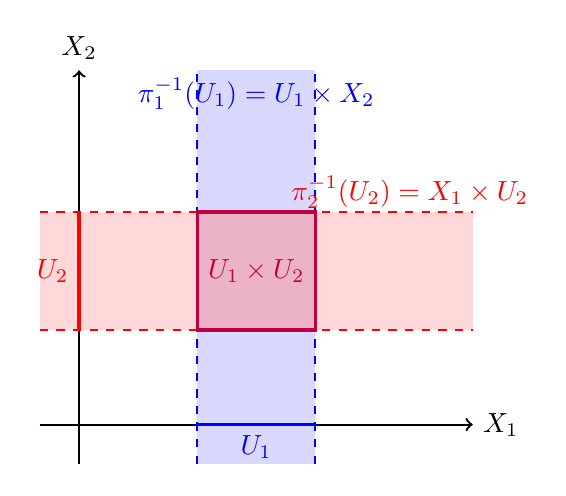
\begin{tikzpicture}[scale=1]
    \draw[->,thick] (-0.5,0) -- (5,0) node[right] {$X_1$};
    \draw[->,thick] (0,-0.5) -- (0,4.5) node[above] {$X_2$};
    
    % Banda vertical \pi_1^{-1}(U_1)
    \fill[blue!15] (1.5,-0.5) rectangle (3,4.5);
    \draw[dashed,blue,thick] (1.5,-0.5) -- (1.5,4.5);
    \draw[dashed,blue,thick] (3,-0.5) -- (3,4.5);
    \node[blue] at (2.25,4.2) {$\pi_1^{-1}(U_1) = U_1 \times X_2$};
    
    % Banda horizontal \pi_2^{-1}(U_2)
    \fill[red!15] (-0.5,1.2) rectangle (5,2.7);
    \draw[dashed,red,thick] (-0.5,1.2) -- (5,1.2);
    \draw[dashed,red,thick] (-0.5,2.7) -- (5,2.7);
    \node[red] at (4.2,2.95) {$\pi_2^{-1}(U_2) = X_1 \times U_2$};
    
    % Intersección U_1 x U_2
    \fill[purple!30] (1.5,1.2) rectangle (3,2.7);
    \draw[purple,very thick] (1.5,1.2) rectangle (3,2.7);
    \node[purple] at (2.25,1.95) {$U_1 \times U_2$};
    
    % Intervalos en los ejes
    \draw[very thick,blue] (1.5,0) -- (3,0) node[midway,below] {$U_1$};
    \draw[very thick,red] (0,1.2) -- (0,2.7) node[midway,left] {$U_2$};
\end{tikzpicture}
\end{center}

\begin{obs}[Topología por cajas vs. Topología producto]
Si en el producto $\prod_{i \in I} X_i$ consideramos la base formada por todos los productos arbitrarios $\prod_{i \in I} U_i$ (sin la restricción de ser $X_i$ para casi todo $i$), se obtiene la \textbf{topología por cajas} (o box topology), denotada $\mc T_{\text{cajas}}$.
\begin{itemize}
    \item En general, $\mc T_\pi \subseteq \mc T_{\text{cajas}}$.
    \item Si el conjunto de índices $I$ es \textbf{finito}, ambas topologías coinciden: $\mc T_\pi = \mc T_{\text{cajas}}$. En particular, en $\mathbb{R}^n = \prod_{i=1}^n \mathbb{R}$, $\mc T_d = \mc T_\pi = \mc T_{\text{cajas}}$.
    \item Si $I$ es \textbf{infinito}, $\mc T_\pi \subsetneq \mc T_{\text{cajas}}$.
\end{itemize}
\end{obs}

\begin{ejem}[Diferencia entre topología producto y por cajas]
Consideremos $X = \mathbb{R}^\mathbb{N} = \prod_{n \in \mathbb{N}} \mathbb{R}$ (el espacio de sucesiones reales). Definamos la aplicación diagonal:
\[
    \Delta \colon (\mathbb{R}, \mc T_d) \longrightarrow \mathbb{R}^\mathbb{N}, \quad x \longmapsto (x, x, x, \ldots).
\]
\begin{itemize}
    \item Con la topología producto $\mc T_\pi$, cada componente $\pi_n \circ \Delta = \operatorname{Id}_\mathbb{R}$ es continua, por lo que por la propiedad universal, $\Delta \colon (\mathbb{R}, \mc T_d) \to (\mathbb{R}^\mathbb{N}, \mc T_\pi)$ es \textbf{continua}.
    \item Con la topología por cajas $\mc T_{\text{cajas}}$, consideremos el abierto por cajas:
    \[
        U = (-1, 1) \times \left(-\frac{1}{2}, \frac{1}{2}\right) \times \ldots \times \left(-\frac{1}{n}, \frac{1}{n}\right) \times \ldots \in \mc T_{\text{cajas}}.
    \]
    Su anti-imagen es $\Delta^{-1}(U) = \bigcap_{n=1}^\infty (-\nicefrac{1}{n}, \nicefrac{1}{n}) = \{0\}$, que \textbf{no} es abierto en $(\mathbb{R}, \mc T_d)$. Así, $\Delta \colon (\mathbb{R}, \mc T_d) \to (\mathbb{R}^\mathbb{N}, \mc T_{\text{cajas}})$ \textbf{no es continua}.
\end{itemize}
\end{ejem}

\subsection*{Topología final}

\begin{defi}
Sea $(X, \mc T_X)$ un espacio topológico, $Y$ un conjunto y $f \colon X \to Y$ una aplicación. La \textbf{topología final} en $Y$ inducida por $f$, denotada $\mc T^f$, es la mayor topología en $Y$ que hace continua a $f$:
\[
    \mc T^f = \{V \subseteq Y \mid f^{-1}(V) \in \mc T_X\}.
\]
Para una familia de aplicaciones $\{f_i \colon (X_i, \mc T_{X_i}) \to Y\}_{i \in I}$, la \textbf{topología final} $\mc T^{\{f_i\}}$ es la mayor topología en $Y$ que hace continuas a todas las $f_i$:
\[
    \mc T^{\{f_i\}} = \bigcap_{i \in I} \mc T^{f_i} = \{V \subseteq Y \mid f_i^{-1}(V) \in \mc T_{X_i}, \; \forall i \in I\}.
\]
\end{defi}

\begin{teo}[Propiedad universal de la topología final]
Sea $Y$ dotado de la topología final $\mc T^{\{f_i\}}$. Para cualquier espacio topológico $(Z, \mc T_Z)$, una aplicación $g \colon (Y, \mc T^{\{f_i\}}) \to (Z, \mc T_Z)$ es continua si y solo si la composición:
\[
    g \circ f_i \colon (X_i, \mc T_{X_i}) \longrightarrow (Z, \mc T_Z)
\]
es continua para todo $i \in I$.
\end{teo}

\begin{dem}
\begin{itemize}
    \item[($\Rightarrow$)] Si $g$ es continua, al ser cada $f_i$ continua, $g \circ f_i$ es continua.
    \item[($\Leftarrow$)] Sea $U \subseteq Z$ abierto. Para ver que $g^{-1}(U) \in \mc T^{\{f_i\}}$, debemos comprobar que $f_i^{-1}(g^{-1}(U)) \in \mc T_{X_i}$ para todo $i \in I$. Pero $f_i^{-1}(g^{-1}(U)) = (g \circ f_i)^{-1}(U)$, que es abierto por ser $g \circ f_i$ continua.
\end{itemize}
\end{dem}

\subsection*{Unión disjunta (Suma topológica)}

\begin{defi}
Dada una familia de espacios topológicos $\{(X_i, \mc T_{X_i})\}_{i \in I}$, el \textbf{espacio unión disjunta} es el coproducto de conjuntos $\coprod_{i \in I} X_i = \{(i, x) \mid i \in I, \; x \in X_i\}$ dotado de la \textbf{topología final} inducida por las inyecciones canónicas:
\[
    \varphi_j \colon X_j \longhookrightarrow \coprod_{i \in I} X_i, \quad x_j \longmapsto (j, x_j).
\]
Un subconjunto $W \subseteq \coprod_{i \in I} X_i$ es abierto si y solo si $\varphi_i^{-1}(W)$ es abierto en $X_i$ para todo $i \in I$. Cada inyección canónica $\varphi_j$ es una inmersión abierta y cerrada.
\end{defi}

\section{Topología cociente}

\begin{defi}
Sea $(X, \mc T_X)$ un espacio topológico y $R$ una relación de equivalencia en $X$. Denotemos por $\pi \colon X \to X/R$ la proyección natural al cociente ($x \mapsto [x]_R$). La \textbf{topología cociente} $\mc T_{X/R}$ es la \textbf{topología final} inducida por $\pi$:
\[
    \mc T_{X/R} = \{V \subseteq X/R \mid \pi^{-1}(V) \in \mc T_X\}.
\]
\end{defi}

\begin{defi}
Sea $R$ una relación de equivalencia en $X$. Un subconjunto $A \subseteq X$ se dice \textbf{saturado} por $R$ si contiene todas las clases de equivalencia de sus elementos:
\[
    \forall a \in A, \quad [a]_R \subseteq A \iff \pi^{-1}(\pi(A)) = A.
\]
Dado cualquier subconjunto $A \subseteq X$, la \textbf{saturación} de $A$ es el menor saturado que contiene a $A$:
\[
    [A]_R := \bigcup_{a \in A} [a]_R = \pi^{-1}(\pi(A)).
\]
\end{defi}

\begin{prop}
La proyección canónica $\pi \colon (X, \mc T_X) \to (X/R, \mc T_{X/R})$ es abierta si y solo si para todo abierto $U \in \mc T_X$, su saturado $[U]_R$ es abierto en $X$.
\end{prop}

\begin{dem}
$\pi(U)$ es abierto en el cociente $\iff \pi^{-1}(\pi(U)) \in \mc T_X \iff [U]_R \in \mc T_X$.
\end{dem}

\begin{ejem}[La recta con dos orígenes]
Consideremos dos copias de la recta real $X = \mathbb{R}_1 \sqcup \mathbb{R}_2$. En $X$ definimos la relación de equivalencia que identifica cada punto $x \in \mathbb{R}_1 \setminus \{0\}$ con su homólogo en $\mathbb{R}_2 \setminus \{0\}$:
\[
    (1, x) \sim (2, y) \iff x = y \ne 0.
\]
En el espacio cociente $X/{\sim}$, el espacio es localmente idéntico a la recta real euclídea salvo en el origen, donde existen dos puntos distintos $0_1 = [(1, 0)]$ y $0_2 = [(2, 0)]$. Este espacio \textbf{no es de Hausdorff ($T_2$)}, pues todo entorno abierto de $0_1$ y todo entorno abierto de $0_2$ intersecan fuera del origen.

\begin{center}
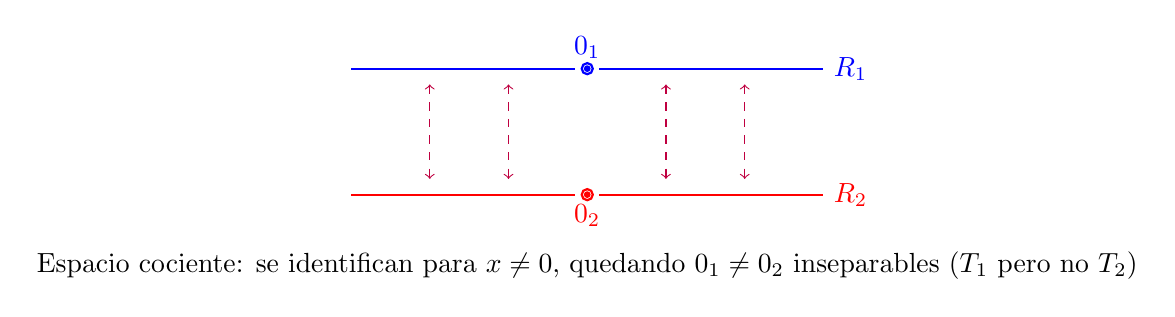
\begin{tikzpicture}[scale=1]
    % Recta R_1 arriba
    \draw[thick,blue] (-3,0.8) -- (-0.15,0.8);
    \draw[thick,blue] (0.15,0.8) -- (3,0.8) node[right] {$\mathbb{R}_1$};
    \draw[thick,blue] (0,0.8) circle (2pt);
    \filldraw[blue] (0,0.8) circle (1pt) node[above] {$0_1$};
    
    % Recta R_2 abajo
    \draw[thick,red] (-3,-0.8) -- (-0.15,-0.8);
    \draw[thick,red] (0.15,-0.8) -- (3,-0.8) node[right] {$\mathbb{R}_2$};
    \draw[thick,red] (0,-0.8) circle (2pt);
    \filldraw[red] (0,-0.8) circle (1pt) node[below] {$0_2$};
    
    % Flechas de pegamiento
    \draw[<->,dashed,purple] (-2,0.6) -- (-2,-0.6);
    \draw[<->,dashed,purple] (-1,0.6) -- (-1,-0.6);
    \draw[<->,dashed,purple] (1,0.6) -- (1,-0.6);
    \draw[<->,dashed,purple] (2,0.6) -- (2,-0.6);
    
    \node at (0,-1.7) [align=center] {Espacio cociente: se identifican para $x \ne 0$, quedando $0_1 \ne 0_2$ inseparables ($T_1$ pero no $T_2$)};
\end{tikzpicture}
\end{center}
\end{ejem}
























\chapter{Espacios m\'etricos}
\section{Métricas, seudométricas e isometrías}

\begin{defi}
Sea $X$ un conjunto. Una \textbf{métrica} (o distancia) en $X$ es una aplicación $d \colon X \times X \to \mathbb{R}$ tal que:
\begin{enumerate}
    \item[\textbf{1)}] $d(x, y) \ge 0$ para todos $x, y \in X$, y $d(x, y) = 0 \iff x = y$.
    \item[\textbf{2)}] $d(x, y) = d(y, x)$ para todos $x, y \in X$ (simetría).
    \item[\textbf{3)}] $d(x, y) \le d(x, z) + d(z, y)$ para todos $x, y, z \in X$ (desigualdad triangular).
\end{enumerate}
Una aplicación $d$ es una \textbf{seudométrica} si verifica las propiedades 2, 3 y la versión debilitada de 1: $d(x, y) \ge 0$ con $x = y \Rightarrow d(x, y) = 0$ (pudiendo ser $d(x, y) = 0$ para puntos distintos $x \ne y$). El par $(X, d)$ se denomina \textbf{espacio métrico} (o seudométrico).
\end{defi}

\begin{ejem}
En $\mathbb{R}^n$, la distancia euclídea usual:
\[
    d(x, y) = \sqrt{\sum_{i=1}^n (x_i - y_i)^2}
\]
es una métrica.
\end{ejem}

\begin{propi}[Métrica acotada asociada]
Sea $(X, d)$ un espacio métrico (o seudométrico). La aplicación:
\[
    \overline{d} \colon X \times X \longrightarrow \mathbb{R}, \quad (x, y) \longmapsto \overline{d}(x, y) := \min\{d(x, y), 1\}
\]
es una métrica (o seudométrica) acotada por $1$.
\end{propi}

\begin{dem}
\begin{itemize}
    \item Claramente $\overline{d}(x, y) \ge 0$, y $\overline{d}(x, y) = 0 \iff d(x, y) = 0 \iff x = y$.
    \item Simetría: $\overline{d}(x, y) = \min\{d(x, y), 1\} = \min\{d(y, x), 1\} = \overline{d}(y, x)$.
    \item Desigualdad triangular: Si $\overline{d}(x, z) = 1$ o $\overline{d}(z, y) = 1$, entonces $\overline{d}(x, z) + \overline{d}(z, y) \ge 1 \ge \overline{d}(x, y)$. Si ambos son menores que $1$, $\overline{d}(x, z) = d(x, z)$ y $\overline{d}(z, y) = d(z, y)$, por lo que $\overline{d}(x, y) \le d(x, y) \le d(x, z) + d(z, y) = \overline{d}(x, z) + \overline{d}(z, y)$.
\end{itemize}
\end{dem}

\begin{defi}
Una \textbf{isometría} entre dos espacios métricos $(X, d)$ e $(Y, d')$ es una aplicación $f \colon X \to Y$ que preserva distancias:
\[
    \forall x, x' \in X, \quad d'(f(x), f(x')) = d(x, x').
\]
Si $d$ es métrica, toda isometría es \textbf{inyectiva}:
\[
    f(x) = f(x') \Rightarrow d'(f(x), f(x')) = 0 \Rightarrow d(x, x') = 0 \Rightarrow x = x'.
\]
Dos espacios métricos son \textbf{isomorfos métricamente} (o isométricos) si existe una isometría biyectiva entre ellos.
\end{defi}

\begin{defi}
Sea $(X, d)$ un espacio métrico. Un subconjunto $A \subseteq X$ es \textbf{acotado} si existe $M \in \mathbb{R}^+$ tal que para todos $a, a' \in A$, $d(a, a') \le M$.
\end{defi}

\begin{defi}
Dado $A \subseteq (X, d)$ no vacío y $x \in X$, la distancia de $x$ a $A$ es:
\[
    d(x, A) := \inf\{d(x, a) \mid a \in A\}.
\]
Esto induce una función $d_A \colon X \to \mathbb{R}$ dada por $x \mapsto d(x, A)$.
\end{defi}

\begin{center}
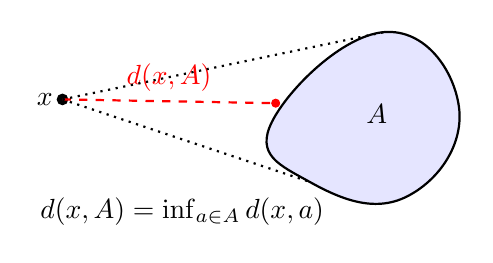
\begin{tikzpicture}[scale=0.95]
    \draw[thick,fill=blue!10] plot[smooth cycle,tension=0.8] coordinates {(2,0) (3.5,1.2) (4.5,0.2) (3.8,-1) (2.5,-0.8)};
    \node at (3.4,0.1) {$A$};
    \filldraw[black] (-0.8,0.3) circle (2pt) node[left] {$x$};
    \draw[dashed,thick,red] (-0.8,0.3) -- (2.05,0.25) node[midway,above] {$d(x, A)$};
    \filldraw[red] (2.05,0.25) circle (1.5pt);
    \draw[dotted,thick] (-0.8,0.3) -- (3.5,1.2);
    \draw[dotted,thick] (-0.8,0.3) -- (2.5,-0.8);
    \node at (0.8,-1.2) [align=center] {$d(x, A) = \inf_{a \in A} d(x, a)$};
\end{tikzpicture}
\end{center}

\begin{ejem}
$\mathbb{N} \subset (\mathbb{R}, d)$ no está acotado. En cambio, en $(\mathbb{R}, \overline{d})$, $\mathbb{N}$ (y todo subconjunto de $\mathbb{R}$) está acotado por $1$.
\end{ejem}

\section{Topología asociada a una métrica}

\begin{defi}
Sea $(X, d)$ un espacio métrico. Dados $x \in X$ y $r \in \mathbb{R}^+$, la \textbf{bola abierta} de centro $x$ y radio $r$ es:
\[
    B_d(x, r) := \{y \in X \mid d(x, y) < r\}.
\]
La familia $\{B_d(x, r)\}_{r > 0}$ constituye una base de entornos en $x$, y la colección de todas las bolas abiertas forma una base de una topología en $X$, denominada la \textbf{topología métrica} $\mc T_d$. Un subconjunto $U \subseteq X$ es abierto en $\mc T_d$ si:
\[
    \forall x \in U, \; \exists r_x > 0 \text{ tal que } B_d(x, r_x) \subseteq U.
\]
\end{defi}

\begin{propi}
Toda bola abierta $B_d(x, r)$ es un conjunto abierto en $(X, \mc T_d)$.
\end{propi}

\begin{dem}
Sea $y \in B_d(x, r)$, luego $d(x, y) < r$. Tomando $r_y := r - d(x, y) > 0$, para cualquier $z \in B_d(y, r_y)$ se tiene por desigualdad triangular $d(x, z) \le d(x, y) + d(y, z) < d(x, y) + r_y = r$, de donde $B_d(y, r_y) \subseteq B_d(x, r)$.
\end{dem}

\begin{center}
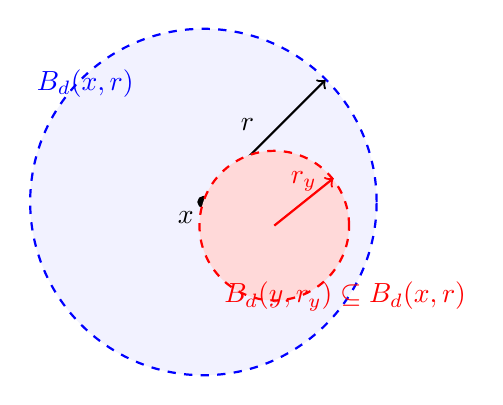
\begin{tikzpicture}[scale=1]
    \draw[thick,blue,dashed,fill=blue!5] (0,0) circle (2.2cm);
    \filldraw[black] (0,0) circle (2pt) node[below left] {$x$};
    \draw[->,thick] (0,0) -- (1.55,1.55) node[midway,above left] {$r$};
    \node[blue] at (-1.5,1.5) {$B_d(x, r)$};
    
    \filldraw[black] (0.9,-0.3) circle (2pt) node[below left] {$y$};
    \draw[thick,red,dashed,fill=red!15] (0.9,-0.3) circle (0.95cm);
    \draw[->,thick,red] (0.9,-0.3) -- (1.65,0.3) node[midway,above] {$r_y$};
    \node[red] at (1.8,-1.2) {$B_d(y, r_y) \subseteq B_d(x, r)$};
\end{tikzpicture}
\end{center}

\begin{defi}
Se define la \textbf{bola cerrada} y la \textbf{esfera} (o circunferencia métrica) de centro $x$ y radio $r$ como:
\begin{align*}
    \overline{B}_d(x, r) &:= \{y \in X \mid d(x, y) \le r\}, \\
    C_d(x, r) &:= \{y \in X \mid d(x, y) = r\}.
\end{align*}
Nótese que $\overline{B}_d(x, r) = B_d(x, r) \cup C_d(x, r)$.
\end{defi}

\begin{prop}
La bola cerrada $\overline{B}_d(x, r)$ es un conjunto cerrado en $(X, \mc T_d)$.
\end{prop}

\begin{dem}
Basta ver que su complementario $X \setminus \overline{B}_d(x, r) = \{y \in X \mid d(x, y) > r\}$ es abierto. Si $y \in X \setminus \overline{B}_d(x, r)$, tomamos $r_y := d(x, y) - r > 0$. Para todo $z \in B_d(y, r_y)$, $d(x, y) \le d(x, z) + d(z, y) < d(x, z) + r_y$, luego $d(x, z) > d(x, y) - r_y = r$, de modo que $B_d(y, r_y) \subseteq X \setminus \overline{B}_d(x, r)$.
\end{dem}

\begin{obs}
En general, el cierre de la bola abierta está contenido en la bola cerrada: $\overline{B_d(x, r)} \subseteq \overline{B}_d(x, r)$, pero \textbf{no siempre} coinciden. Por ejemplo, en $(\mathbb{R}^n, \overline{d})$, $B_{\overline{d}}(0, 2) = \mathbb{R}^n$, luego $\overline{B_{\overline{d}}(0, 2)} = \mathbb{R}^n$, mientras que para métricas discretas pueden diferir estrictamente.
\end{obs}

\begin{cor}
La familia de bolas cerradas $\{\overline{B}_d(x, r)\}_{r > 0}$ forma una base de entornos cerrados de $x$.
\end{cor}

\section{Espacios metrizables}

\begin{defi}
Un espacio topológico $(X, \mc T)$ es \textbf{metrizable} si existe una métrica $d$ en $X$ tal que $\mc T = \mc T_d$.
\end{defi}

\begin{teo}[Teorema de metrización de Urysohn]
Todo espacio topológico regular ($T_3$), $T_0$ y con base numerable de abiertos (segundo contable) es metrizable.
\end{teo}

\begin{prop}
Sea $(X, d)$ un espacio métrico y $\overline{d}(x, y) = \min\{1, d(x, y)\}$. Entonces:
\[
    \mc T_d = \mc T_{\overline{d}}.
\]
\end{prop}

\begin{dem}
Como $\overline{d}(x, y) \le d(x, y)$, para $r \le 1$ se tiene $B_d(x, r) = B_{\overline{d}}(x, r)$, lo que muestra que ambas métricas generan las mismas bolas para radios pequeños y por tanto la misma topología.
\end{dem}

\begin{prop}
Si $(X, \mc T)$ es metrizable ($\mc T = \mc T_d$ para una seudométrica $d$), son equivalentes:
\begin{enumerate}
    \item[\textbf{1)}] $(X, \mc T)$ es $T_2$ (Hausdorff).
    \item[\textbf{2)}] $(X, \mc T)$ es $T_0$.
    \item[\textbf{3)}] $d$ es métrica.
\end{enumerate}
\end{prop}

\begin{dem}
$1 \Rightarrow 2$ es general. Para $2 \Rightarrow 3$: si $x \ne y$, por ser $T_0$ existe un entorno abierto de uno que no contiene al otro, luego existe $\varepsilon > 0$ con $y \notin B_d(x, \varepsilon)$, lo que implica $d(x, y) \ge \varepsilon > 0$. Para $3 \Rightarrow 1$: si $x \ne y$, como $d$ es métrica $\varepsilon := d(x, y) > 0$. Las bolas $B_d(x, \varepsilon/2)$ y $B_d(y, \varepsilon/2)$ son disjuntas por desigualdad triangular, luego $X$ es $T_2$.
\end{dem}

\begin{center}
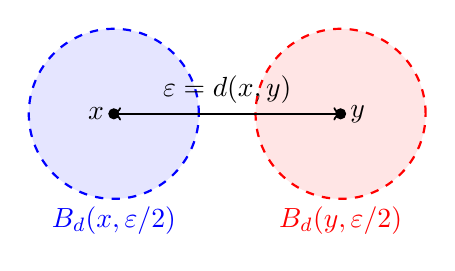
\begin{tikzpicture}[scale=0.9]
    \draw[thick,blue,dashed,fill=blue!10] (0,0) circle (1.2cm);
    \draw[thick,red,dashed,fill=red!10] (3.2,0) circle (1.2cm);
    \filldraw[black] (0,0) circle (2pt) node[left] {$x$};
    \filldraw[black] (3.2,0) circle (2pt) node[right] {$y$};
    \draw[<->,thick] (0,0) -- (3.2,0) node[midway,above] {$\varepsilon = d(x, y)$};
    \node[blue] at (0,-1.5) {$B_d(x, \varepsilon/2)$};
    \node[red] at (3.2,-1.5) {$B_d(y, \varepsilon/2)$};
\end{tikzpicture}
\end{center}

\subsection*{Sucesiones y caracterizaciones secuenciales}

\begin{prop}
En un espacio métrico $(X, d)$, una sucesión $\{x_n\}$ converge a $x \iff \lim_{n \to \infty} d(x, x_n) = 0$.
\end{prop}

\begin{prop}
Sea $(X, \mc T_d)$ un espacio metrizable y $A \subseteq X$. Un punto $x \in \overline{A} \iff$ existe una sucesión $\{x_n\} \subseteq A$ tal que $\lim_{n \to \infty} x_n = x$.
\end{prop}

\begin{dem}
($\Rightarrow$) Para cada $n \in \mathbb{N}$, como $x \in \overline{A}$, la bola $B_d(x, \nicefrac{1}{n})$ corta a $A$. Escogiendo $x_n \in B_d(x, \nicefrac{1}{n}) \cap A$, se construye una sucesión $\{x_n\} \subseteq A$ con $d(x, x_n) < \nicefrac{1}{n} \to 0$.

($\Leftarrow$) Es válido en cualquier espacio topológico: si $x_n \to x$ con $\{x_n\} \subseteq A$, todo entorno de $x$ contiene puntos de $\{x_n\} \subseteq A$, luego $x \in \overline{A}$.
\end{dem}

\begin{prop}
Sean $(X, \mc T_X)$ un espacio metrizable e $(Y, \mc T_Y)$ un espacio topológico arbitrario. Una aplicación $f \colon X \to Y$ es continua si y solo si para toda sucesión $\{x_n\} \subseteq X$ que converge a $x$, la sucesión $\{f(x_n)\}$ converge a $f(x)$ en $Y$.
\end{prop}

\begin{dem}
($\Rightarrow$) Si $f$ es continua y $W$ es entorno de $f(x)$, $f^{-1}(W)$ es entorno de $x$. Como $x_n \to x$, existe $n_0$ con $x_n \in f^{-1}(W)$ para todo $n \ge n_0$, luego $f(x_n) \in W$.

($\Leftarrow$) Sea $C \subseteq Y$ cerrado. Si probamos que $\overline{f^{-1}(C)} = f^{-1}(C)$, habremos demostrado que $f^{-1}(C)$ es cerrado. Sea $x \in \overline{f^{-1}(C)}$; por la caracterización secuencial existe $\{x_n\} \subseteq f^{-1}(C)$ con $x_n \to x$. Entonces $\{f(x_n)\} \subseteq C$, y por hipótesis $f(x_n) \to f(x)$. Como $C$ es cerrado, $f(x) \in C$, luego $x \in f^{-1}(C)$.
\end{dem}

\begin{prop}
Sean $(X, d)$ e $(Y, d')$ espacios métricos. Una aplicación $f \colon X \to Y$ es continua $\iff$ para todo $x \in X$ y todo $\varepsilon > 0$, existe $\delta_{x, \varepsilon} > 0$ tal que:
\[
    d(x, x') < \delta_{x, \varepsilon} \Rightarrow d'(f(x), f(x')) < \varepsilon \iff B_d(x, \delta_{x, \varepsilon}) \subseteq f^{-1}(B_{d'}(f(x), \varepsilon)).
\]
\end{prop}

\section{Continuidad uniforme y separabilidad}

\begin{defi}
Una aplicación $f \colon (X, d) \to (Y, d')$ es \textbf{uniformemente continua} si para todo $\varepsilon > 0$ existe $\delta_\varepsilon > 0$ (independiente del punto $x$) tal que:
\[
    \forall x, x' \in X, \quad d(x, x') < \delta_\varepsilon \Rightarrow d'(f(x), f(x')) < \varepsilon.
\]
Toda aplicación uniformemente continua es continua.
\end{defi}

\begin{propi}
Sea $(X, d)$ un espacio métrico y $A \subseteq X$ no vacío. La función distancia al subconjunto:
\[
    d_A \colon X \longrightarrow \mathbb{R}, \quad x \longmapsto d(x, A) = \inf_{a \in A} d(x, a)
\]
es uniformemente continua (y en particular, continua).
\end{propi}

\begin{dem}
Para cualesquiera $x, x' \in X$ y $a \in A$: $d(x, a) \le d(x, x') + d(x', a)$. Tomando ínfimo sobre $a \in A$, $d(x, A) \le d(x, x') + d(x', a)$, de donde $d(x, A) - d(x', A) \le d(x, x')$. Por simetría:
\[
    |d(x, A) - d(x', A)| \le d(x, x').
\]
Basta tomar $\delta_\varepsilon = \varepsilon$.
\end{dem}

\begin{defi}
Un espacio topológico $X$ es \textbf{separable} si contiene un subconjunto denso y numerable: existe $Y \subseteq X$ numerable tal que $\overline{Y} = X$.
\end{defi}

\begin{ejem}
$\mathbb{R}$ es separable, pues $\mathbb{Q} \subset \mathbb{R}$ es numerable y $\overline{\mathbb{Q}} = \mathbb{R}$.
\end{ejem}

\begin{propi}
Todo espacio métrico separable $(X, d)$ tiene una base numerable de abiertos (es segundo contable).
\end{propi}

\begin{dem}
Sea $Y = \{x_n\}_{n \in \mathbb{N}}$ un subconjunto numerable denso en $X$. Consideremos la familia numerable de bolas:
\[
    \mathcal{B} = \{B_d(x_n, 1/m) \mid n, m \in \mathbb{N}\}.
\]
Dado cualquier abierto $U$ y $x \in U$, existe $r > 0$ con $B_d(x, r) \subseteq U$. Tomando $m \in \mathbb{N}$ tal que $1/m < r/2$, por la densidad de $Y$ existe $x_n \in Y$ con $d(x, x_n) < 1/m$. Entonces $x \in B_d(x_n, 1/m) \subseteq B_d(x, r) \subseteq U$. Luego $\mathcal{B}$ es base numerable.
\end{dem}

\begin{cor}
$\mathbb{R}^n$ es separable (mediante $\mathbb{Q}^n$) y tiene base numerable de abiertos: $\{B_d(q, 1/m) \mid q \in \mathbb{Q}^n, \; m \in \mathbb{N}\}$.
\end{cor}

\section{Espacios métricos $\mathbb{R}^n$ y métricas equivalentes}

\begin{teo}
$(\mathbb{R}^n, \mc T_\pi)$ es metrizable.
\end{teo}

\begin{dem}
Definimos la distancia del máximo en $\mathbb{R}^n$:
\[
    d_{\max}(x, y) := \max_{1 \le i \le n} |x_i - y_i|.
\]
Probemos que $\mc T_\pi = \mc T_{d_{\max}}$:
\begin{itemize}
    \item[($\subseteq$)] Sea $U = U_1 \times \ldots \times U_n \in \mc T_\pi$ un abierto básico y $x \in U$. Para cada $i$, como $U_i \in \mc T_d$, existe $\varepsilon_i > 0$ tal que $(x_i - \varepsilon_i, x_i + \varepsilon_i) \subseteq U_i$. Tomando $\varepsilon = \min_{1 \le i \le n} \varepsilon_i > 0$, si $y \in B_{d_{\max}}(x, \varepsilon)$, entonces $|x_i - y_i| \le d_{\max}(x, y) < \varepsilon \le \varepsilon_i$, luego $y_i \in U_i$ para todo $i$, y $B_{d_{\max}}(x, \varepsilon) \subseteq U$.
    \item[($\supseteq$)] Sea $x \in \mathbb{R}^n$ y $\varepsilon > 0$. El producto $U = B_{d_1}(x_1, \varepsilon) \times \ldots \times B_{d_1}(x_n, \varepsilon)$ es un abierto básico de $\mc T_\pi$ que contiene a $x$ y cumple $U \subseteq B_{d_{\max}}(x, \varepsilon)$.
\end{itemize}
\end{dem}

\begin{prop}
En $\mathbb{R}^n$ consideramos las siguientes cuatro métricas:
\begin{enumerate}
    \item[\textbf{a)}] $d(x, y) = \sqrt{\sum_{i=1}^n |x_i - y_i|^2}$ (euclídea).
    \item[\textbf{b)}] $\overline{d}(x, y) = \min\{1, d(x, y)\}$.
    \item[\textbf{c)}] $d_{\max}(x, y) = \max_{1 \le i \le n} |x_i - y_i|$.
    \item[\textbf{d)}] $d_{\text{suma}}(x, y) = \sum_{i=1}^n |x_i - y_i|$ (de Manhattan).
\end{enumerate}
Todas ellas inducen la misma topología:
\[
    \mc T_{\overline{d}} = \mc T_d = \mc T_{d_{\text{suma}}} = \mc T_{d_{\max}} = \mc T_\pi.
\]
\end{prop}

\begin{dem}
Para todos $x, y \in \mathbb{R}^n$:
\[
    d_{\max}^2(x, y) = \max_{1 \le i \le n} |x_i - y_i|^2 \le \sum_{i=1}^n |x_i - y_i|^2 = d^2(x, y) \le \left(\sum_{i=1}^n |x_i - y_i|\right)^2 = d_{\text{suma}}^2(x, y).
\]
Tomando raíces cuadradas: $d_{\max}(x, y) \le d(x, y) \le d_{\text{suma}}(x, y)$. Además:
\[
    d_{\text{suma}}(x, y) = \sum_{i=1}^n |x_i - y_i| \le n \max_{1 \le i \le n} |x_i - y_i| = n \, d_{\max}(x, y).
\]
Por tanto, $B_{d_{\text{suma}}}(x, \varepsilon) \subseteq B_d(x, \varepsilon) \subseteq B_{d_{\max}}(x, \varepsilon)$, y $B_{d_{\max}}(x, \varepsilon/n) \subseteq B_{d_{\text{suma}}}(x, \varepsilon)$, lo que demuestra que las topologías coinciden.
\end{dem}

\begin{center}
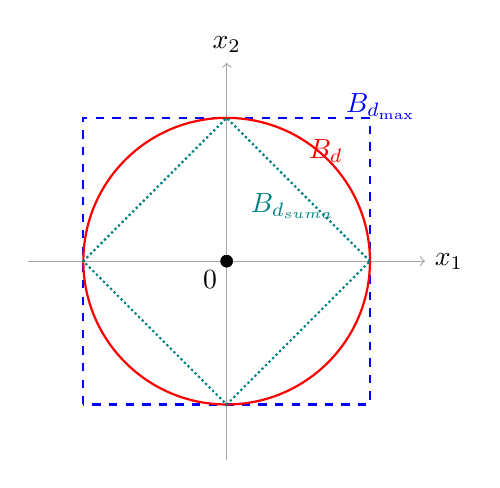
\begin{tikzpicture}[scale=1.4]
    \draw[->,gray!70] (-1.8,0) -- (1.8,0) node[right,black] {$x_1$};
    \draw[->,gray!70] (0,-1.8) -- (0,1.8) node[above,black] {$x_2$};
    
    % Bola máximo (cuadrado)
    \draw[thick,blue,dashed] (-1.3,-1.3) rectangle (1.3,1.3);
    \node[blue] at (1.4,1.4) {$B_{d_{\max}}$};
    
    % Bola euclídea (círculo)
    \draw[thick,red] (0,0) circle (1.3cm);
    \node[red] at (0.9,1) {$B_d$};
    
    % Bola suma (rombo)
    \draw[thick,teal,densely dotted] (1.3,0) -- (0,1.3) -- (-1.3,0) -- (0,-1.3) -- cycle;
    \node[teal] at (0.6,0.5) {$B_{d_{\text{suma}}}$};
    
    \filldraw[black] (0,0) circle (1.5pt) node[below left] {$0$};
\end{tikzpicture}
\end{center}

\section{Metrizabilidad de $\mathbb{R}^\mathbb{N}$}

\begin{teo}
El espacio producto numerable $(\mathbb{R}^\mathbb{N}, \mc T_\pi)$ (espacio de sucesiones de números reales dotado de la topología producto) es metrizable.
\end{teo}

\begin{dem}
En $\mathbb{R}$ consideramos la métrica acotada $\overline{d}(a, b) = \min\{1, |a - b|\} \le 1$. Para $x = (x_n)_{n \in \mathbb{N}}$ e $y = (y_n)_{n \in \mathbb{N}}$ en $\mathbb{R}^\mathbb{N}$, definimos:
\[
    D(x, y) := \sup_{n \in \mathbb{N}} \left\{ \frac{\overline{d}(x_n, y_n)}{n} \right\} \le 1.
\]
\begin{enumerate}
    \item[\textbf{1)}] $D(x, y) \ge 0$. Si $D(x, y) = 0 \iff \frac{\overline{d}(x_n, y_n)}{n} = 0$ para todo $n \iff x_n = y_n$ para todo $n \iff x = y$.
    \item[\textbf{2)}] Simetría: inmediata por la simetría de $\overline{d}$.
    \item[\textbf{3)}] Desigualdad triangular: Para cada $n \in \mathbb{N}$, $\frac{\overline{d}(x_n, y_n)}{n} \le \frac{\overline{d}(x_n, z_n)}{n} + \frac{\overline{d}(z_n, y_n)}{n} \le D(x, z) + D(z, y)$. Tomando supremo en $n$, $D(x, y) \le D(x, z) + D(z, y)$.
\end{enumerate}
Luego $D$ es una métrica en $\mathbb{R}^\mathbb{N}$. Veamos que $\mc T_\pi = \mc T_D$:
\begin{itemize}
    \item[($\mc T_\pi \subseteq \mc T_D$)] Basta probar que cada abierto de la subbase $\pi_N^{-1}(B_{\overline{d}}(x_N, \varepsilon))$ contiene una bola abierta $B_D(x, \delta)$. Tomando $\delta = \frac{\varepsilon}{N} > 0$: si $y \in B_D(x, \delta)$, entonces $\frac{\overline{d}(x_N, y_N)}{N} \le D(x, y) < \frac{\varepsilon}{N}$, luego $\overline{d}(x_N, y_N) < \varepsilon$, de donde $y \in \pi_N^{-1}(B_{\overline{d}}(x_N, \varepsilon))$.
    \item[($\mc T_D \subseteq \mc T_\pi$)] Sea $x \in \mathbb{R}^\mathbb{N}$ y $\varepsilon > 0$. Elegimos $N \in \mathbb{N}$ tal que $\frac{1}{N} < \varepsilon$. Definimos el abierto de $\mc T_\pi$:
    \[
        U = (x_1 - \varepsilon, x_1 + \varepsilon) \times \ldots \times (x_N - \varepsilon, x_N + \varepsilon) \times \prod_{n > N} \mathbb{R}.
    \]
    Para todo $y \in U$:
    \begin{itemize}
        \item Si $n \le N$: $\frac{\overline{d}(x_n, y_n)}{n} \le \overline{d}(x_n, y_n) < \varepsilon$.
        \item Si $n > N$: $\frac{\overline{d}(x_n, y_n)}{n} \le \frac{1}{n} < \frac{1}{N} < \varepsilon$.
    \end{itemize}
    Por tanto, $D(x, y) = \sup_{n} \frac{\overline{d}(x_n, y_n)}{n} \le \varepsilon$, lo que implica $U \subseteq B_D(x, 2\varepsilon)$. Consecuentemente, $\mc T_D = \mc T_\pi$.
\end{itemize}
\end{dem}

\begin{obs}
\begin{itemize}
    \item Con la topología por cajas $\mc T_{\text{cajas}}$, el espacio $(\mathbb{R}^\mathbb{N}, \mc T_{\text{cajas}})$ \textbf{no} es metrizable.
    \item Si el conjunto de índices $I$ no es numerable, el producto $(\mathbb{R}^I, \mc T_\pi)$ \textbf{no} es metrizable.
\end{itemize}
\end{obs}


































\chapter{Espacios conexos}
Sea $X$ un espacio topológico.

\section{Espacios conexos y separaciones}

\begin{defi}
Una \textbf{separación} de un espacio topológico $X$ es un par de abiertos no vacíos y disjuntos $(A, B)$ tales que:
\[
    X = A \cup B, \quad A \ne \emptyset, \; B \ne \emptyset, \quad A \cap B = \emptyset.
\]
Equivalentemente, $A$ y $B$ son subconjuntos complementarios no triviales que son simultáneamente abiertos y cerrados (clopen). Se llama \textbf{separación trivial} a la pareja $(\emptyset, X)$ o $(X, \emptyset)$.
\end{defi}

\begin{defi}
Un espacio topológico $X$ es \textbf{conexo} si no admite ninguna separación no trivial; es decir, los únicos subconjuntos de $X$ que son simultáneamente abiertos y cerrados son $\emptyset$ y $X$.
\end{defi}

\begin{defi}
Un subespacio topológico $Y \subseteq X$ es conexo si lo es dotado de la topología relativa $(Y, \mc T_{X|Y})$.
\end{defi}

\begin{ejem}
\begin{itemize}
    \item La recta real $\mathbb{R}$ dotada de la topología habitual es conexa.
    \item El subespacio $X = [-2, -1] \cup [1, 2] \subset \mathbb{R}$ no es conexo, pues $[-2, -1] = (-3, 0) \cap X$ y $[1, 2] = (0, 3) \cap X$ constituyen una separación no trivial por abiertos relativos.
\end{itemize}
\end{ejem}

\begin{prop}
Sea $Y \subseteq X$ un subespacio conexo y sea $(A, B)$ una separación de $X$. Entonces:
\[
    Y \subseteq A \quad \text{o bien} \quad Y \subseteq B.
\]
\end{prop}

\begin{dem}
Como $X = A \cup B$ con $A \cap B = \emptyset$, tenemos:
\[
    Y = (A \cap Y) \cup (B \cap Y), \quad (A \cap Y) \cap (B \cap Y) = \emptyset.
\]
Al ser $A$ y $B$ abiertos en $X$, $A \cap Y$ y $B \cap Y$ son abiertos en $Y$. Por ser $Y$ conexo, esta separación relativa debe ser trivial, de modo que $A \cap Y = \emptyset$ (y así $Y \subseteq B$) o $B \cap Y = \emptyset$ (y así $Y \subseteq A$).
\end{dem}

\begin{prop}
Sea $Y \subseteq X$ un subespacio conexo. Para todo subespacio $Z \subseteq X$ tal que $Y \subseteq Z \subseteq \overline{Y}$, $Z$ es conexo. En particular, la clausura $\overline{Y}$ de todo subespacio conexo es conexa.
\end{prop}

\begin{dem}
Sea $(A, B)$ una separación de $Z$ por cerrados relativos: $Z = A \cup B$ con $A \cap B = \emptyset$. Existen cerrados $\overline{A}, \overline{B}$ en $X$ con $A = \overline{A} \cap Z$ y $B = \overline{B} \cap Z$. Como $Y \subseteq Z$ es conexo, por la proposición anterior $Y \subseteq A$ o $Y \subseteq B$. Si $Y \subseteq A$, entonces $\overline{Y} \subseteq \overline{A}$, y por tanto:
\[
    Z \subseteq \overline{Y} \cap Z \subseteq \overline{A} \cap Z = A.
\]
Esto implica $B = \emptyset$, por lo que la separación de $Z$ es trivial y $Z$ es conexo.
\end{dem}

\begin{prop}
Sea $\{X_i\}_{i \in I}$ una familia de subespacios conexos de $X$ tales que su intersección común es no vacía: $\bigcap_{i \in I} X_i \ne \emptyset$. Entonces:
\[
    \bigcup_{i \in I} X_i \quad \text{es conexo}.
\]
\end{prop}

\begin{dem}
Sea $(A, B)$ una separación de $\bigcup_{i \in I} X_i$. Fijemos un punto $x \in \bigcap_{i \in I} X_i$. Sin pérdida de generalidad, supongamos $x \in A$. Para cada $j \in I$, como $X_j$ es conexo, $X_j \subseteq A$ o $X_j \subseteq B$. Puesto que $x \in X_j \cap A$, necesariamente $X_j \subseteq A$ para todo $j \in I$. En consecuencia, $\bigcup_{j \in I} X_j \subseteq A$, lo que obliga a $B = \emptyset$.
\end{dem}

\begin{ejem}
Si dos subespacios disjuntos no se cortan, su unión en general no es conexa. Por ejemplo, en $\mathbb{R}^2$ tomemos dos rectas verticales distintas $X_1 = \{x_1\} \times \mathbb{R}$ y $X_2 = \{x_2\} \times \mathbb{R}$ con $x_1 \ne x_2$. La unión $X_1 \cup X_2$ no es conexa.

\begin{center}
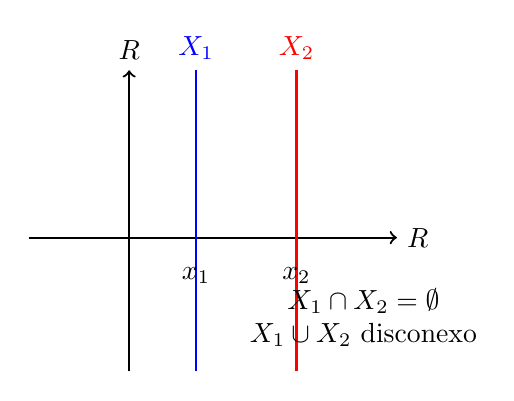
\begin{tikzpicture}[scale=0.85]
    \draw[->,thick] (-1.5,0) -- (4,0) node[right] {$\mathbb{R}$};
    \draw[->,thick] (0,-2) -- (0,2.5) node[above] {$\mathbb{R}$};
    \draw[thick,blue] (1,-2) -- (1,2.5) node[above] {$X_1$};
    \draw[thick,red] (2.5,-2) -- (2.5,2.5) node[above] {$X_2$};
    \node at (1,-0.3) [below] {$x_1$};
    \node at (2.5,-0.3) [below] {$x_2$};
    \node at (3.5,-1.2) [align=center] {$X_1 \cap X_2 = \emptyset$ \\ $X_1 \cup X_2$ disconexo};
\end{tikzpicture}
\end{center}
\end{ejem}

\subsection*{Conexión en la recta real}

\begin{defi}
Un subconjunto $A \subseteq \mathbb{R}$ es un \textbf{intervalo} si para cualesquiera $a, b \in A$ con $a < b$, se verifica $[a, b] \subseteq A$.
\end{defi}

\begin{prop}
Los únicos subespacios conexos de $(\mathbb{R}, \mc T_d)$ son los puntos unitarios y los intervalos.
\end{prop}

\begin{dem}
\begin{itemize}
    \item[($\Rightarrow$)] Sea $A \subseteq \mathbb{R}$ conexo con más de un punto. Si $A$ no fuera un intervalo, existirían $a < b \in A$ y un punto $c \notin A$ tal que $a < c < b$. Entonces $U_1 = (-\infty, c)$ y $U_2 = (c, \infty)$ son abiertos disjuntos de $\mathbb{R}$ que inducen una separación no trivial en $A$:
    \[
        A = (A \cap (-\infty, c)) \cup (A \cap (c, \infty)),
    \]
    ya que $a \in A \cap U_1$ y $b \in A \cap U_2$, contradiciendo que $A$ es conexo.
    \item[($\Leftarrow$)] Todo punto unitario es conexo. Supongamos que $A$ es un intervalo y que $A = U_1 \cup U_2$ con $U_1, U_2$ abiertos relativos disjuntos y no vacíos. Sean $a \in U_1$ y $b \in U_2$ con $a < b$. Como $A$ es intervalo, $[a, b] \subseteq A$. Es suficiente ver que $[a, b] \cong [0, 1]$ es conexo. Supongamos $[0, 1] = U_1 \cup U_2$ con $0 \in U_1$. Sea $r = \sup \{t \in [0, 1] \mid [0, t] \subseteq U_1\}$. Si $r \in U_1$, como $U_1$ es abierto existe $\varepsilon > 0$ con $[r, r+\varepsilon) \subseteq U_1$, contradiciendo que $r$ es cota superior. Si $r \in U_2$, por apertura existe $\varepsilon' > 0$ con $(r-\varepsilon', r] \subseteq U_2$, contradiciendo que $r$ es la menor cota superior. Por tanto, $[0, 1]$ es conexo y todo intervalo es conexo.
\end{itemize}
\end{dem}

\section{Preservación de la conexión y Teorema del Valor Medio}

\begin{prop}
Sea $f \colon X \to Y$ una aplicación continua. Si $X$ es conexo, entonces su imagen $\operatorname{Im}(f) = f(X)$ es un subespacio conexo de $Y$. En particular, si $A \subseteq X$ es conexo, $f(A)$ es conexo en $Y$.
\end{prop}

\begin{dem}
Consideremos la correstricción continua $\tilde{f} \colon X \to \operatorname{Im}(f)$. Si $\operatorname{Im}(f) = V_1 \cup V_2$ fuera una separación abierta no trivial, entonces:
\[
    X = \tilde{f}^{-1}(V_1) \cup \tilde{f}^{-1}(V_2)
\]
sería una separación abierta no trivial de $X$, contradiciendo su conexión.
\end{dem}

\begin{cor}[Teorema del valor intermedio]
Sea $X$ un espacio conexo y $f \colon X \to \mathbb{R}$ continua. Si $a, b \in \operatorname{Im}(f)$ con $a < b$, entonces para todo valor $c \in [a, b]$ existe un punto $x \in X$ tal que $f(x) = c$.
\end{cor}

\begin{dem}
Como $X$ es conexo, su imagen $\operatorname{Im}(f) \subseteq \mathbb{R}$ es conexa, luego es un intervalo. Si $a, b \in \operatorname{Im}(f)$, por definición de intervalo $[a, b] \subseteq \operatorname{Im}(f)$.
\end{dem}

\begin{teo}
Sea $\{X_i\}_{i \in I}$ una familia de espacios topológicos. El producto $\prod_{i \in I} X_i$ es conexo si y solo si cada $X_j$ es conexo.
\end{teo}

\begin{dem}
($\Rightarrow$) Como las proyecciones canónicas $\pi_j \colon \prod X_i \to X_j$ son continuas y sobreyectivas, la imagen $\pi_j(\prod X_i) = X_j$ es conexa.

($\Leftarrow$) Consideremos primero el caso finito $n = 2$: $X_1 \times X_2$. Fijemos un punto base $b = (b_1, b_2) \in X_1 \times X_2$. Para cada $x_1 \in X_1$, el subespacio en forma de ``cruz'':
\[
    C_{x_1} := (\{x_1\} \times X_2) \cup (X_1 \times \{b_2\})
\]
es conexo, pues $\{x_1\} \times X_2 \cong X_2$ y $X_1 \times \{b_2\} \cong X_1$ son conexos y se cortan en el punto $(x_1, b_2)$. Además, para todo $x_1 \in X_1$, $b \in C_{x_1}$, por lo que:
\[
    X_1 \times X_2 = \bigcup_{x_1 \in X_1} C_{x_1}
\]
es una unión de conexos con intersección no vacía, luego es conexo.

\begin{center}
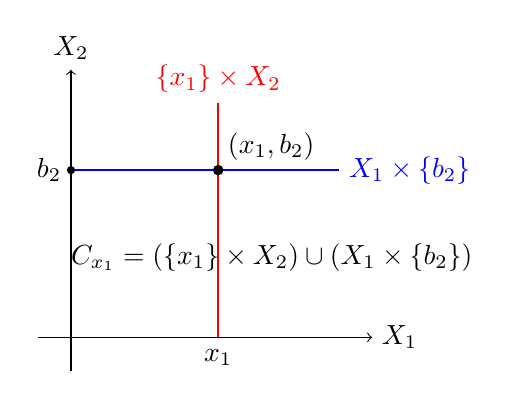
\begin{tikzpicture}[scale=0.85]
    \draw[->] (-0.5,0) -- (4.5,0) node[right] {$X_1$};
    \draw[->] (0,-0.5) -- (0,4) node[above] {$X_2$};
    \draw[thick,blue] (0,2.5) -- (4,2.5) node[right] {$X_1 \times \{b_2\}$};
    \draw[thick,red] (2.2,0) -- (2.2,3.5) node[above] {$\{x_1\} \times X_2$};
    \filldraw[black] (2.2,2.5) circle (2pt) node[above right] {$(x_1, b_2)$};
    \filldraw[black] (0,2.5) circle (1.5pt) node[left] {$b_2$};
    \node at (2.2,-0.3) {$x_1$};
    \node at (3,1.2) [align=center] {$C_{x_1} = (\{x_1\} \times X_2) \cup (X_1 \times \{b_2\})$};
\end{tikzpicture}
\end{center}

Por inducción, todo producto finito $\prod_{i=1}^n X_i$ es conexo. Para $I$ arbitrario, fijemos $b = (b_i)_{i \in I}$. Para cada subconjunto finito $M \subset I$, definimos:
\[
    F^M := \left\{(x_i)_{i \in I} \in \prod_{i \in I} X_i \;\middle|\; x_i = b_i, \; \forall i \notin M\right\} \cong \prod_{i \in M} X_i.
\]
Cada $F^M$ es conexo y contiene a $b$. Entonces $Y = \bigcup_{M \subset I \text{ finito}} F^M$ es conexo. Dado cualquier abierto básico no vacío $U$ de la topología producto, $U$ restringe solo un número finito de coordenadas, por lo que corta a algún $F^M \subseteq Y$. Así, $Y$ es denso en $\prod X_i$. Por tanto, $\prod_{i \in I} X_i = \overline{Y}$ es conexo.
\end{dem}

\begin{cor}
$\mathbb{R}^n$ y $\mathbb{R}^\mathbb{N}$ son espacios conexos.
\end{cor}

\begin{obs}
La unión disjunta $\coprod_{i \in I} X_i$ con $|I| \ge 2$ \textbf{nunca} es conexa, pues cada componente $\varphi_j(X_j)$ es abierta y cerrada a la vez.
\end{obs}

\section{Componentes conexas}

Sea $X$ un espacio topológico. Se define la siguiente relación en $X$:
\[
    x \sim y \iff \text{existe un subespacio conexo } A \subseteq X \text{ tal que } x, y \in A.
\]

\begin{propi}
La relación $\sim$ es una relación de equivalencia:
\begin{enumerate}
    \item \textbf{Reflexiva:} $x \sim x$, ya que $\{x\}$ es conexo.
    \item \textbf{Simétrica:} Si $x, y \in A$ conexo, $y, x \in A$.
    \item \textbf{Transitiva:} Si $x \sim y$ ($x, y \in A$ conexo) e $y \sim z$ ($y, z \in B$ conexo), como $y \in A \cap B \ne \emptyset$, $A \cup B$ es conexo y $x, z \in A \cup B$.
\end{enumerate}
\end{propi}

\begin{defi}
Las clases de equivalencia de la relación $\sim$ se denominan \textbf{componentes conexas} de $X$. La componente conexa de un punto $x$ se denota $[x] = C_x$.
\end{defi}

\begin{lema}
Si $A \subseteq X$ es un subespacio conexo y $x \in A$, entonces $A \subseteq [x]$.
\end{lema}

\begin{prop}
Las componentes conexas de $X$ son los subespacios conexos maximales de $X$. Además, son disjuntas y particionan $X$: $X = \bigsqcup C_i$.
\end{prop}

\begin{dem}
Cada clase $[x] = \bigcup \{A \subseteq X \text{ conexo} \mid x \in A\}$ es conexa por ser unión de conexos con el punto $x$ en común. Si $C \subseteq K$ con $K$ conexo, tomando $x \in C$ se tiene $K \subseteq [x] = C$, luego es maximal.
\end{dem}

\begin{prop}
Toda componente conexa $C$ de un espacio topológico $X$ es un conjunto \textbf{cerrado}: $C = \overline{C}$.
\end{prop}

\begin{dem}
Como $C$ es conexo, su clausura $\overline{C}$ es conexa. Por la maximalidad de $C$, $C \subseteq \overline{C} \Rightarrow C = \overline{C}$.
\end{dem}

\begin{obs}
En general, las componentes conexas \textbf{no} son abiertas. Sin embargo, si $X$ tiene un número finito de componentes conexas $X = C_1 \cup \ldots \cup C_n$, entonces cada $C_i = X \setminus \bigcup_{j \ne i} C_j$ es el complementario de una unión finita de cerrados, luego cada $C_i$ es simultáneamente abierta y cerrada.
\end{obs}

\begin{ejem}
\begin{itemize}
    \item En $(X, \mc T_{\text{discreta}})$, los únicos subespacios conexos son los puntos aislados $\{x\}$. Las componentes conexas son los puntos unitarios, por lo que $X$ es \textbf{totalmente disconexo}.
    \item En la recta de Sorgenfrey $(\mathbb{R}, \mc T_{\text{Sorg}})$, para todo punto $a \in Y \subseteq \mathbb{R}$, $Y = (Y \cap (-\infty, a)) \cup (Y \cap [a, \infty))$ define una separación abierta relativa si existen puntos a izquierda y derecha de $a$. Por tanto, $(\mathbb{R}, \mc T_{\text{Sorg}})$ es totalmente disconexo.
\end{itemize}
\end{ejem}

\section{Espacios arcoconexos (Conexión por caminos)}

\begin{defi}
Sea $X$ un espacio topológico y $x, x' \in X$. Un \textbf{camino} (o arco) en $X$ que une $x$ con $x'$ es una aplicación continua:
\[
    \gamma \colon [0, 1] \longrightarrow X \quad \text{tal que } \gamma(0) = x, \; \gamma(1) = x'.
\]
Dados dos caminos continuos $\gamma_1, \gamma_2 \colon [0, 1] \to X$ tales que $\gamma_1(1) = \gamma_2(0) = x'$, se define la \textbf{concatenación} (o suma de caminos) $\gamma_1 * \gamma_2 \colon [0, 1] \to X$:
\[
    (\gamma_1 * \gamma_2)(t) = \begin{cases} \gamma_1(2t) & \text{si } 0 \le t \le \frac{1}{2}, \\ \gamma_2(2t - 1) & \text{si } \frac{1}{2} \le t \le 1. \end{cases}
\]
Por el lema de pegamiento cerrado, $\gamma_1 * \gamma_2$ es continua y define un camino que une $\gamma_1(0)$ con $\gamma_2(1)$.
\end{defi}

\begin{center}
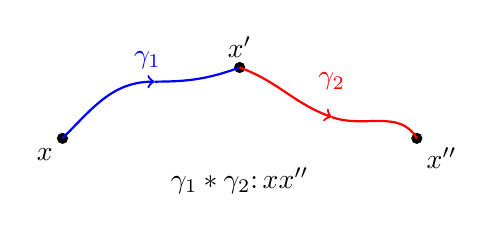
\begin{tikzpicture}[scale=0.9]
    \filldraw[black] (0,0) circle (2pt) node[below left] {$x$};
    \filldraw[black] (2.5,1) circle (2pt) node[above] {$x'$};
    \filldraw[black] (5,0) circle (2pt) node[below right] {$x''$};
    \draw[thick,blue,->] (0,0) to[out=45,in=180] (1.3,0.8);
    \draw[thick,blue] (1.3,0.8) to[out=0,in=200] (2.5,1);
    \node[blue] at (1.2,1.1) {$\gamma_1$};
    \draw[thick,red,->] (2.5,1) to[out=-20,in=160] (3.8,0.3);
    \draw[thick,red] (3.8,0.3) to[out=-20,in=120] (5,0);
    \node[red] at (3.8,0.8) {$\gamma_2$};
    \node at (2.5,-0.6) {$\gamma_1 * \gamma_2 \colon x \rightsquigarrow x''$};
\end{tikzpicture}
\end{center}

\begin{defi}
Un espacio topológico $X$ es \textbf{arcoconexo} (o conexo por caminos) si para cualesquiera dos puntos $x, x' \in X$, existe un camino en $X$ que une $x$ con $x'$.
\end{defi}

\begin{teo}
Todo espacio arcoconexo es conexo.
\end{teo}

\begin{dem}
Supongamos que $X$ admite una separación no trivial $X = U \cup U'$ con $U \cap U' = \emptyset$ y $U, U' \ne \emptyset$. Sean $x \in U$ y $x' \in U'$. Como $X$ es arcoconexo, existe un camino continuo $\gamma \colon [0, 1] \to X$ con $\gamma(0) = x$ y $\gamma(1) = x'$. La imagen $\gamma([0, 1])$ es conexa, pero:
\[
    \gamma([0, 1]) = (\gamma([0, 1]) \cap U) \cup (\gamma([0, 1]) \cap U')
\]
constituye una separación no trivial de $\gamma([0, 1])$, contradicción.
\end{dem}

\begin{prop}
Si $f \colon X \to Y$ es continua y $X$ es arcoconexo, $\operatorname{Im}(f)$ es un subespacio arcoconexo de $Y$.
\end{prop}

\begin{dem}
Dados $y, y' \in \operatorname{Im}(f)$, existen $x, x' \in X$ con $f(x) = y$ y $f(x') = y'$. Si $\gamma \colon [0, 1] \to X$ es un camino entre $x$ y $x'$, entonces $f \circ \gamma \colon [0, 1] \to \operatorname{Im}(f)$ es continua y une $y$ con $y'$.
\end{dem}

\begin{ejem}[Contraejemplos: conexo $\not\Rightarrow$ arcoconexo]
\textbf{1. Seno del topólogo:} Sea $\Gamma_f$ la gráfica de $f(x) = \sin(1/x)$ en $(0, \infty)$:
\[
    \Gamma_f = \left\{\left(x, \sin\frac{1}{x}\right) \;\middle|\; x > 0\right\} \subset \mathbb{R}^2.
\]
$\Gamma_f$ es arcoconexo (es imagen continua de $(0, \infty)$), luego conexo. Su clausura en $\mathbb{R}^2$ es:
\[
    \overline{\Gamma}_f = \Gamma_f \cup (\{0\} \times [-1, 1]).
\]
$\overline{\Gamma}_f$ es conexo (por ser clausura de un conexo), pero \textbf{no es arcoconexo}: no existe ningún camino continuo que conecte el origen $(0, 0)$ con un punto de la gráfica $\Gamma_f$.

\begin{center}
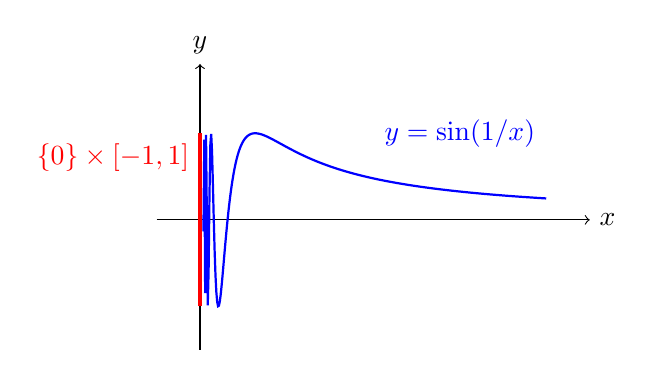
\begin{tikzpicture}[scale=1.1]
    \draw[->] (-0.5,0) -- (4.5,0) node[right] {$x$};
    \draw[->] (0,-1.5) -- (0,1.8) node[above] {$y$};
    \draw[very thick,red] (0,-1) -- (0,1) node[below left] {$\{0\} \times [-1, 1]$};
    \draw[domain=0.04:4,samples=400,variable=\x,blue,thick] 
        plot ({\x}, {sin((1/\x)*180/pi)});
    \node[blue] at (3,1) {$y = \sin(1/x)$};
\end{tikzpicture}
\end{center}

\textbf{2. Peine del topólogo:} En $\mathbb{R}^2$, consideremos:
\[
    P = ([0, 1] \times \{0\}) \cup \left(\bigcup_{n=1}^\infty \left\{\frac{1}{n}\right\} \times [0, 1]\right).
\]
$P$ es arcoconexo. El espacio $Y = P \cup \{(0, 1)\}$ es conexo (pues $P \subset Y \subset \overline{P}$), pero \textbf{no es arcoconexo}, ya que el punto $(0, 1)$ no puede unirse por camino a ningún otro punto de $Y$.

\begin{center}
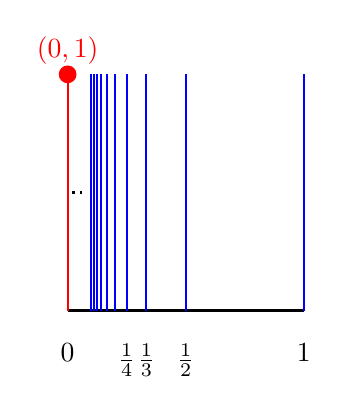
\begin{tikzpicture}[scale=3]
    \draw[thick] (0,0) -- (1,0);
    \foreach \n in {1, 2, 3, 4, 5, 6, 7, 8, 9, 10} {
        \draw[thick,blue] ({1/\n}, 0) -- ({1/\n}, 1);
    }
    \draw[thick,dotted] (0.02, 0.5) -- (0.08, 0.5);
    \draw[thick,red] (0,0) -- (0,1);
    \filldraw[red] (0,1) circle (1pt) node[above] {$(0, 1)$};
    \node at (1,-0.1) [below] {$1$};
    \node at (0.5,-0.1) [below] {$\frac{1}{2}$};
    \node at (0.333,-0.1) [below] {$\frac{1}{3}$};
    \node at (0.25,-0.1) [below] {$\frac{1}{4}$};
    \node at (0,-0.1) [below] {$0$};
\end{tikzpicture}
\end{center}
\end{ejem}

\section{Espacios localmente conexos y arcoconexos}

\begin{defi}
Un espacio topológico $X$ es \textbf{localmente conexo} (resp. \textbf{localmente arcoconexo}) si para todo punto $x \in X$ y todo abierto $U$ con $x \in U$, existe un abierto conexo (resp. arcoconexo) $V$ tal que $x \in V \subseteq U$.
\end{defi}

\begin{teo}
Un espacio $X$ es localmente conexo (resp. arcoconexo) si y solo si las componentes conexas (resp. arcoconexas) de cualquier abierto de $X$ son abiertas.
\end{teo}

\begin{cor}
Si $X$ es localmente conexo (o localmente arcoconexo), sus componentes conexas (o arcoconexas) son simultáneamente abiertas y cerradas.
\end{cor}

\begin{teo}
Si $X$ es un espacio conexo y localmente arcoconexo, entonces $X$ es arcoconexo. Además, en cualquier espacio localmente arcoconexo, las componentes conexas coinciden con las componentes arcoconexas.
\end{teo}

\begin{dem}
Sea $x_0 \in X$ y sea $Q_{x_0}$ la componente arcoconexa de $x_0$. Como $X$ es localmente arcoconexo, $Q_{x_0}$ es abierta. De igual modo, su complementario $X \setminus Q_{x_0} = \bigcup_{y \notin Q_{x_0}} Q_y$ es unión de abiertos, luego es abierto. Siendo $Q_{x_0} \ne \emptyset$ abierto y cerrado en el espacio conexo $X$, se concluye que $Q_{x_0} = X$, por lo que $X$ es arcoconexo.
\end{dem}

\section{Homotopía y grupo fundamental}

\begin{defi}
Sea $X$ un espacio topológico y $x \in X$. Un \textbf{lazo} con base en $x$ es un camino continuo $\gamma \colon [0, 1] \to X$ tal que $\gamma(0) = \gamma(1) = x$.
\end{defi}

\begin{defi}
Dos caminos $\gamma, \gamma' \colon [0, 1] \to X$ con los mismos extremos ($\gamma(0) = \gamma'(0)$ y $\gamma(1) = \gamma'(1)$) son \textbf{homótopos} (relativo a los extremos) si existe una aplicación continua:
\[
    H \colon [0, 1] \times [0, 1] \longrightarrow X
\]
tal que para todos $t, s \in [0, 1]$:
\begin{align*}
    H(t, 0) &= \gamma(t), \quad H(t, 1) = \gamma'(t), \\
    H(0, s) &= \gamma(0), \quad H(1, s) = \gamma(1).
\end{align*}
La relación de homotopía $\sim$ es una relación de equivalencia en la familia de lazos basados en $x$.
\end{defi}

\begin{center}
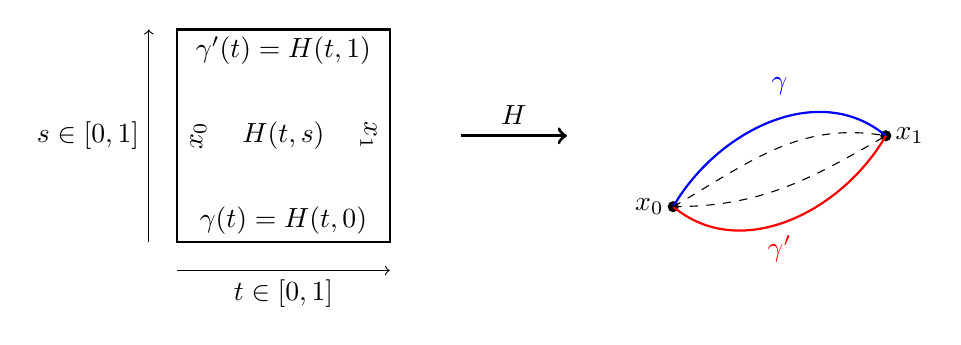
\begin{tikzpicture}[scale=0.9]
    \draw[thick] (0,0) rectangle (3,3);
    \draw[->] (0,-0.4) -- (3,-0.4) node[midway,below] {$t \in [0, 1]$};
    \draw[->] (-0.4,0) -- (-0.4,3) node[midway,left] {$s \in [0, 1]$};
    \node at (1.5,0.3) {$\gamma(t) = H(t, 0)$};
    \node at (1.5,2.7) {$\gamma'(t) = H(t, 1)$};
    \node at (0.3,1.5) [rotate=90] {$x_0$};
    \node at (2.7,1.5) [rotate=-90] {$x_1$};
    \node at (1.5,1.5) {$H(t, s)$};
    
    \draw[->,very thick] (4,1.5) -- (5.5,1.5) node[midway,above] {$H$};
    
    \begin{scope}[shift={(7,0.5)}]
        \filldraw[black] (0,0) circle (2pt) node[left] {$x_0$};
        \filldraw[black] (3,1) circle (2pt) node[right] {$x_1$};
        \draw[thick,blue] (0,0) to[out=60,in=140] (3,1);
        \draw[thick,red] (0,0) to[out=-40,in=-120] (3,1);
        \draw[dashed] (0,0) to[out=30,in=170] (3,1);
        \draw[dashed] (0,0) to[out=0,in=-150] (3,1);
        \node[blue] at (1.5,1.7) {$\gamma$};
        \node[red] at (1.5,-0.6) {$\gamma'$};
    \end{scope}
\end{tikzpicture}
\end{center}

\begin{defi}
El conjunto de clases de homotopía de lazos basados en $x$, dotado de la concatenación $[\gamma] \cdot [\gamma'] = [\gamma * \gamma']$, forma un grupo denominado el \textbf{grupo fundamental} de $X$ en el punto base $x$, denotado $\pi_1(X, x)$. El elemento neutro es la clase del lazo constante $e_x(t) = x$, y el inverso de $[\gamma]$ es la clase del lazo recorrido en sentido inverso $\gamma^{-1}(t) = \gamma(1 - t)$.
\end{defi}

\begin{prop}
Si $X$ es arcoconexo, para cualesquiera $x, x' \in X$ se verifica $\pi_1(X, x) \cong \pi_1(X, x')$, por lo que se escribe $\pi_1(X)$.
\end{prop}

\begin{ejem}
\begin{itemize}
    \item $\pi_1(\mathbb{R}^n) = \{0\}$.
    \item $\pi_1(\mathbb{R}^2 \setminus \{(0, 0)\}) \cong \pi_1(S^1) \cong \mathbb{Z}$.
    \item $\pi_1(S^2) = \{0\}$.
    \item $\pi_1(\mathbb{T}^2) \cong \mathbb{Z} \times \mathbb{Z}$ para el toro 2-dimensional.
\end{itemize}
\end{ejem}

\begin{defi}
Un espacio topológico $X$ es \textbf{simplemente conexo} si es arcoconexo y su grupo fundamental es trivial: $\pi_1(X) = \{0\}$.
\end{defi}

\section{Espacios irreducibles}

\begin{defi}
Un espacio topológico $X$ es \textbf{irreducible} si no se puede expresar como unión de dos subconjuntos cerrados propios:
\[
    X = C_1 \cup C_2 \text{ con } C_1, C_2 \text{ cerrados} \Rightarrow X = C_1 \quad \text{o} \quad X = C_2.
\]
\end{defi}

\begin{prop}
En cualquier espacio topológico $X$, son equivalentes:
\begin{enumerate}
    \item[\textbf{1)}] $X$ es irreducible.
    \item[\textbf{2)}] Dos abiertos no vacíos cualesquiera se cortan siempre: $U, V \in \mc T \setminus \{\emptyset\} \Rightarrow U \cap V \ne \emptyset$.
    \item[\textbf{3)}] Todo abierto no vacío $U$ es denso en $X$: $\overline{U} = X$.
\end{enumerate}
\end{prop}

\begin{dem}
\begin{itemize}
    \item[\textbf{1 $\iff$ 2:}] Sean $U, V$ abiertos. $(X \setminus U) \cup (X \setminus V) = X \setminus (U \cap V)$. Por definición de irreducibilidad, esta unión de cerrados es todo $X \iff X \setminus U = X$ o $X \setminus V = X$, es decir, $U \cap V = \emptyset \iff U = \emptyset$ o $V = \emptyset$.
    \item[\textbf{2 $\iff$ 3:}] $U$ es denso $\iff$ todo abierto no vacío corta a $U$.
\end{itemize}
\end{dem}

\begin{obs}
\begin{itemize}
    \item Todo espacio irreducible es conexo. El recíproco es falso: $\mathbb{R}^2$ euclídeo es conexo pero no es irreducible (por ejemplo, dos abiertos disjuntos no se cortan).
    \item Un espacio de Hausdorff ($T_2$) es irreducible si y solo si consta de a lo sumo un punto.
    \item La topología de Zariski en geometría algebraica da lugar a espacios irreducibles estándar.
\end{itemize}
\end{obs}

\begin{ejem}
\begin{itemize}
    \item En $(\mathbb{R}, \mc T_{\text{kol}})$ con $\mc T_{\text{kol}} = \{(a, \infty) \mid a \in \mathbb{R}\} \cup \{\emptyset, \mathbb{R}\}$, cualesquiera dos abiertos $(a, \infty) \cap (b, \infty) = (\max\{a, b\}, \infty) \ne \emptyset$, luego $(\mathbb{R}, \mc T_{\text{kol}})$ es irreducible.
    \item La unión de los dos ejes coordenados en el plano afín $X = \{(x, y) \mid xy = 0\} = C_1 \cup C_2$ no es irreducible, siendo sus componentes irreducibles las rectas $C_1 = \{y = 0\}$ y $C_2 = \{x = 0\}$.
\end{itemize}

\begin{center}
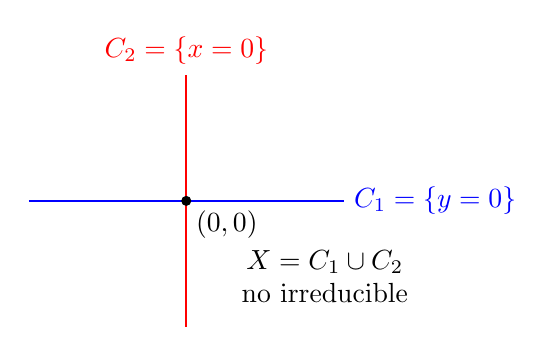
\begin{tikzpicture}[scale=0.8]
    \draw[thick,blue] (-2.5,0) -- (2.5,0) node[right] {$C_1 = \{y=0\}$};
    \draw[thick,red] (0,-2) -- (0,2) node[above] {$C_2 = \{x=0\}$};
    \filldraw[black] (0,0) circle (2pt) node[below right] {$(0, 0)$};
    \node at (2.2,-1.2) [align=center] {$X = C_1 \cup C_2$ \\ no irreducible};
\end{tikzpicture}
\end{center}
\end{ejem}


































\chapter{Espacios topol\'ogicos compactos}Sea \(X\) un espacio topológico.

\section{Espacios Compactos y Subespacios}

\begin{defi}
Sea \(X\) un espacio topológico:
\begin{itemize}
    \item Un \textbf{recubrimiento abierto} de \(X\) es una familia de abiertos \(\{U_i\}_{i \in I}\) de \(X\) tal que \(X = \bigcup_{i \in I} U_i\).
    \item Un \textbf{subrecubrimiento} de \(\{U_i\}_{i \in I}\) es una subfamilia \(\{U_j\}_{j \in J}\) con \(J \subseteq I\) tal que \(X = \bigcup_{j \in J} U_j\).
    \item Un \textbf{refinamiento} de \(\{U_i\}_{i \in I}\) es un recubrimiento abierto \(\{V_j\}_{j \in J}\) tal que para cada \(j \in J\) existe \(i(j) \in I\) con \(V_j \subseteq U_{i(j)}\).
\end{itemize}
\end{defi}

\begin{defi}
Un espacio topológico \(X\) es \textbf{compacto} si todo recubrimiento abierto de \(X\) admite un subrecubrimiento finito:
\[
    X = \bigcup_{i \in I} U_i \Rightarrow \exists i_1, \ldots, i_r \in I \quad \text{tal que} \quad X = \bigcup_{j=1}^r U_{i_j}.
\]
Un subespacio \(Y \subseteq X\) es compacto si lo es con su topología relativa; equivalentemente, para toda familia de abiertos \(\{U_i\}_{i \in I}\) en \(X\) tal que \(Y \subseteq \bigcup_{i \in I} U_i\), existen \(i_1, \ldots, i_r \in I\) tales que \(Y \subseteq \bigcup_{j=1}^r U_{i_j}\).
\end{defi}

\begin{ejem}
\((\mathbb{R}, \mc T_d)\) no es compacto: el recubrimiento \(\mathbb{R} = \bigcup_{n \in \mathbb{Z}} (n - 1, n + 1)\) no admite ningún subrecubrimiento finito.
\end{ejem}

\begin{prop}
Sea \(X\) un espacio topológico compacto y sea \(Y \subseteq X\) un subconjunto cerrado. Entonces \(Y\) es compacto.
\end{prop}

\begin{dem}
Sea \(\{U_i\}_{i \in I}\) una familia de abiertos de \(X\) que recubren a \(Y\), es decir, \(Y \subseteq \bigcup_{i \in I} U_i\). Como \(Y\) es cerrado en \(X\), su complementario \(V := X \setminus Y\) es abierto en \(X\). Entonces la colección \(\{U_i\}_{i \in I} \cup \{V\}\) constituye un recubrimiento abierto de todo el espacio \(X\). Por ser \(X\) compacto, existen índices \(i_1, \ldots, i_r \in I\) tales que:
\[
    X = U_{i_1} \cup \ldots \cup U_{i_r} \cup V.
\]
Intersecando con \(Y\) (y observando que \(V \cap Y = \emptyset\)), obtenemos:
\[
    Y \subseteq U_{i_1} \cup \ldots \cup U_{i_r}.
\]
Por consiguiente, \(Y\) es compacto.
\end{dem}

\begin{prop}
Sea \(X\) un espacio topológico de Hausdorff (\(T_2\)) e \(Y \subseteq X\) un subespacio compacto. Para todo punto \(x \notin Y\), existen abiertos disjuntos \(U_x, U_Y \subseteq X\) tales que \(x \in U_x\) e \(Y \subseteq U_Y\). En particular, \(Y\) es cerrado en \(X\).
\end{prop}

\begin{dem}
Sea \(x \notin Y\). Para cada \(y \in Y\), como \(x \ne y\) y el espacio \(X\) es separado (\(T_2\)), existen abiertos disjuntos \(U_x^y \ni x\) y \(U_y \ni y\) tales que \(U_x^y \cap U_y = \emptyset\). La familia \(\{U_y\}_{y \in Y}\) es un recubrimiento abierto del subespacio compacto \(Y\). Por compacidad, existen \(y_1, \ldots, y_r \in Y\) tales que:
\[
    Y \subseteq U_Y := U_{y_1} \cup \ldots \cup U_{y_r}.
\]
Definimos ahora el conjunto:
\[
    U_x := \bigcap_{j=1}^r U_x^{y_j},
\]
el cual es abierto por ser intersección finita de abiertos y contiene a \(x\). Comprobamos que son disjuntos:
\[
    U_x \cap U_Y = U_x \cap \left(\bigcup_{j=1}^r U_{y_j}\right) = \bigcup_{j=1}^r (U_x \cap U_{y_j}) \subseteq \bigcup_{j=1}^r (U_x^{y_j} \cap U_{y_j}) = \emptyset.
\]
Para probar que \(Y\) es cerrado, observamos que para todo punto \(x \notin Y\) hemos encontrado un abierto \(U_x\) tal que \(x \in U_x \subseteq X \setminus Y\). Por consiguiente, \(X \setminus Y\) es abierto en \(X\), de donde \(Y\) es cerrado.
\end{dem}

\begin{teo}
\begin{enumerate}
    \item[\textbf{a)}] Si \(X\) es compacto e \(Y \subseteq X\) es cerrado, entonces \(Y\) es compacto.
    \item[\textbf{b)}] Si \(X\) es de Hausdorff (\(T_2\)) e \(Y \subseteq X\) es compacto, entonces \(Y\) es cerrado.
    \item[\textbf{c)}] Si \(X\) es compacto y \(T_2\), un subespacio \(Y \subseteq X\) es compacto si y solo si \(Y\) es cerrado.
\end{enumerate}
\end{teo}

\begin{prop}
Sea \(f \colon X \to Y\) una aplicación continua. Si \(X\) es compacto, entonces su imagen \(\operatorname{Im}(f) = f(X) \subseteq Y\) es un subespacio compacto de \(Y\).
\end{prop}

\begin{dem}
Sea \(\{V_i\}_{i \in I}\) un recubrimiento abierto de \(\operatorname{Im}(f)\) en \(Y\): \(\operatorname{Im}(f) \subseteq \bigcup_{i \in I} V_i\). Aplicando la anti-imagen \(f^{-1}\):
\[
    X = f^{-1}(\operatorname{Im}(f)) \subseteq f^{-1}\left(\bigcup_{i \in I} V_i\right) = \bigcup_{i \in I} f^{-1}(V_i).
\]
Al ser \(f\) continua, cada \(f^{-1}(V_i)\) es un abierto de \(X\). Como \(X\) es compacto, existen \(i_1, \ldots, i_r \in I\) tales que:
\[
    X = \bigcup_{j=1}^r f^{-1}(V_{i_j}).
\]
Aplicando la imagen directa:
\[
    \operatorname{Im}(f) = f(X) = f\left(\bigcup_{j=1}^r f^{-1}(V_{i_j})\right) = \bigcup_{j=1}^r f(f^{-1}(V_{i_j})) \subseteq \bigcup_{j=1}^r V_{i_j}.
\]
Por consiguiente, \(\operatorname{Im}(f)\) es compacto.
\end{dem}

\begin{cor}
\(\mathbb{R}^n\) no es compacto para ningún \(n \ge 1\).
\end{cor}

\begin{dem}
La proyección canónica sobre la primera coordenada \(\pi_1 \colon \mathbb{R}^n \to \mathbb{R}\) es continua y sobreyectiva. Si \(\mathbb{R}^n\) fuese compacto, su imagen continua \(\operatorname{Im}(\pi_1) = \mathbb{R}\) sería compacta, lo cual es falso.
\end{dem}

\section{Compacidad en \(\mathbb{R}\) y \(\mathbb{R}^n\)}

\begin{prop}
Para cualesquiera \(a < b \in \mathbb{R}\), el intervalo cerrado \([a, b]\) es compacto en \((\mathbb{R}, \mc T_d)\).
\end{prop}

\begin{dem}
Sea \(\{U_i\}_{i \in I}\) una familia de abiertos de \(\mathbb{R}\) tal que \([a, b] \subseteq \bigcup_{i \in I} U_i\). Como \(a \in [a, b]\), existe algún \(i_0 \in I\) con \(a \in U_{i_0}\). Por apertura de \(U_{i_0}\), existe \(\varepsilon > 0\) tal que \([a, a + \varepsilon) \subseteq U_{i_0}\). Consideramos el conjunto:
\[
    C := \{x \in [a, b] \mid [a, x] \text{ está recubierto por un número finito de abiertos } U_i\}.
\]
El conjunto \(C\) es no vacío (pues \(a \in C\) y \([a, a + \varepsilon) \subseteq C\)) y está acotado superiormente por \(b\). Por el axioma del supremo de los números reales, existe \(c := \sup(C) \le b\).

Veamos primero que \(c \in C\). Como \(c \in [a, b]\), existe \(j_0 \in I\) con \(c \in U_{j_0}\). Al ser \(U_{j_0}\) abierto, existe \(\delta > 0\) tal que \((c - \delta, c + \delta) \subseteq U_{j_0}\). Al ser \(c = \sup(C)\), existe algún elemento \(x \in C\) con \(c - \delta < x \le c\). Por pertenecer a \(C\), \([a, x]\) está recubierto por un número finito de abiertos \(U_{i_1}, \ldots, U_{i_m}\). Como \([x, c] \subseteq (c - \delta, c + \delta) \subseteq U_{j_0}\), se deduce que:
\[
    [a, c] = [a, x] \cup [x, c] \subseteq U_{i_1} \cup \ldots \cup U_{i_m} \cup U_{j_0},
\]
lo cual demuestra que \([a, c]\) admite un subrecubrimiento finito, es decir, \(c \in C\).

Veamos ahora que \(c = b\). Si fuera \(c < b\), tomando \(\delta' := \min\{\delta/2, b - c\} > 0\), el intervalo \([c, c + \delta'] \subseteq U_{j_0}\), con lo cual \([a, c + \delta'] = [a, c] \cup [c, c + \delta']\) admitiría un recubrimiento finito, implicando que \(c + \delta' \in C\). Pero \(c + \delta' > c = \sup(C)\), contradicción. Así pues, \(c = b \in C\), concluyendo que \([a, b]\) es compacto.
\end{dem}

\begin{cor}
En \((\mathbb{R}, \mc T_d)\), un subespacio \(Y \subseteq \mathbb{R}\) es compacto si y solo si es cerrado y acotado.
\end{cor}

\begin{dem}
\begin{itemize}
    \item[(\(\Rightarrow\))] Sea \(Y \subseteq \mathbb{R}\) compacto. Puesto que \((\mathbb{R}, \mc T_d)\) es de Hausdorff (\(T_2\)), por la Propiedad 1.2 \(Y\) es cerrado. Por otra parte, \(\mathbb{R} = \bigcup_{n \in \mathbb{N}} B_d(0, n) = \bigcup_{n \in \mathbb{N}} (-n, n)\), luego \(Y \subseteq \bigcup_{n \in \mathbb{N}} B_d(0, n)\). Al ser \(Y\) compacto, existen \(n_1, \ldots, n_r \in \mathbb{N}\) tales que:
    \[
        Y \subseteq \bigcup_{j=1}^r B_d(0, n_j) = B_d(0, M) = (-M, M),
    \]
    donde \(M := \max\{n_1, \ldots, n_r\}\). En consecuencia, \(Y\) es acotado.
    \item[(\(\Leftarrow\))] Supongamos que \(Y\) es cerrado y acotado. Por ser acotado, existen \(a, b \in \mathbb{R}\) tales que \(Y \subseteq [a, b]\). Como \([a, b]\) es compacto en \(\mathbb{R}\) e \(Y\) es un subconjunto cerrado de \([a, b]\), por la Propiedad 1.1 deducimos que \(Y\) es compacto.
\end{itemize}
\end{dem}

\subsection{El lema del entorno tubular y Teorema de Tychonoff}

\begin{lema}[Lema del tubo o del entorno tubular]
Sean \(X, Y\) espacios topológicos con \(Y\) compacto. Sea \(x_0 \in X\) y sea \(U \subseteq X \times Y\) un abierto tal que \(\{x_0\} \times Y \subseteq U\). Entonces existe un abierto \(W_{x_0} \subseteq X\) con \(x_0 \in W_{x_0}\) tal que:
\[
    W_{x_0} \times Y \subseteq U.
\]
\end{lema}

\begin{dem}
Sea \(y \in Y\). El punto \((x_0, y) \in \{x_0\} \times Y \subseteq U\). Como los productos de abiertos forman una base de la topología de \(X \times Y\), existen abiertos \(U_{x_0}^y \subseteq X\) y \(V_y \subseteq Y\) tales que:
\[
    (x_0, y) \in U_{x_0}^y \times V_y \subseteq U.
\]
La colección \(\{V_y\}_{y \in Y}\) es un recubrimiento por abiertos de \(Y\). Siendo \(Y\) compacto, existen puntos \(y_1, \ldots, y_r \in Y\) tales que \(Y = \bigcup_{j=1}^r V_{y_j}\). Definimos:
\[
    W_{x_0} := \bigcap_{j=1}^r U_{x_0}^{y_j}.
\]
\(W_{x_0}\) es abierto por ser intersección finita de abiertos, y contiene a \(x_0\) porque cada \(U_{x_0}^{y_j}\) lo contiene. Comprobemos que \(W_{x_0} \times Y \subseteq U\): sea \((x, y) \in W_{x_0} \times Y\). Como \(y \in Y = \bigcup_{j=1}^r V_{y_j}\), existe algún \(j \in \{1, \ldots, r\}\) tal que \(y \in V_{y_j}\). Puesto que \(x \in W_{x_0} \subseteq U_{x_0}^{y_j}\), se sigue que:
\[
    (x, y) \in U_{x_0}^{y_j} \times V_{y_j} \subseteq U.
\]
Por lo tanto, \(W_{x_0} \times Y \subseteq U\).
\end{dem}

\begin{center}
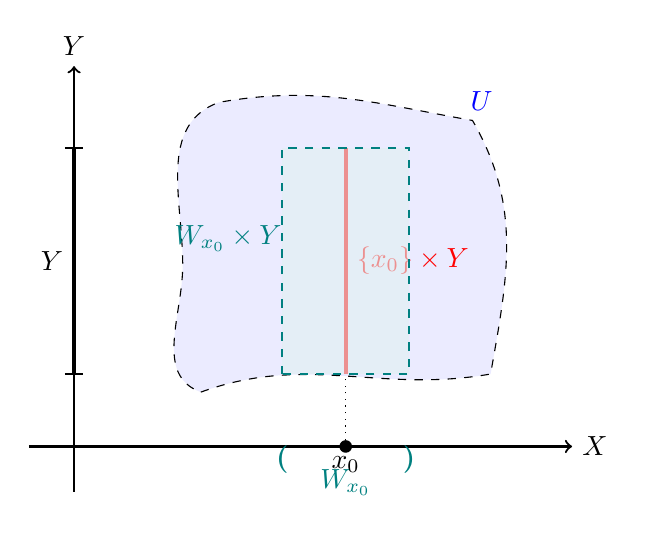
\begin{tikzpicture}[scale=1.15]
    % Ejes coordenados X e Y
    \draw[->,thick] (-0.5,0) -- (5.5,0) node[right] {\(X\)};
    \draw[->,thick] (0,-0.5) -- (0,4.2) node[above] {\(Y\)};
    
    % Abierto U grande que envuelve la fibra
    \draw[dashed,fill=blue!8] 
        (1.4,0.6) to[out=20,in=190] (4.6,0.8) 
        to[out=80,in=-60] (4.4,3.6) 
        to[out=170,in=10] (1.6,3.8) 
        to[out=200,in=90] (1.2,2)
        to[out=-90,in=160] cycle;
    \node[blue] at (4.5,3.6) [above] {\(U\)};
    
    % Fibra vertical {x_0} x Y
    \draw[line width=1.5pt,red] (3,0.8) -- (3,3.3) node[midway,right] {\(\{x_0\} \times Y\)};
    \filldraw[black] (3,0) circle (1.8pt) node[below] {\(x_0\)};
    \draw[dotted] (3,0) -- (3,0.8);
    
    % Paréntesis del abierto W en el eje X
    \draw[thick,teal] (2.3,-0.15) node {\textbf{(}} (3.7,-0.15) node {\textbf{)}};
    \node[teal] at (3,-0.4) {\(W_{x_0}\)};
    
    % Rectángulo tubular W x Y
    \draw[thick,teal,dashed,fill=teal!12,fill opacity=0.6] (2.3,0.8) rectangle (3.7,3.3);
    \node[teal] at (2.4,2.3) [left] {\(W_{x_0} \times Y\)};
    
    % Proyecciones de Y en el eje vertical
    \draw[thick] (-0.1,0.8) -- (0.1,0.8);
    \draw[thick] (-0.1,3.3) -- (0.1,3.3);
    \draw[very thick] (0,0.8) -- (0,3.3) node[midway,left] {\(Y\)};
\end{tikzpicture}
\qquad
\begin{tikzpicture}[scale=0.9]
    \draw[->,thick] (-2.2,0) -- (2.2,0) node[right] {\(x\)};
    \draw[->,thick] (0,-2.2) -- (0,2.2) node[above] {\(y\)};
    
    % Hiperbola xy=1
    \draw[thick,blue,domain=0.45:2,samples=60] plot (\x, {1/\x});
    \draw[thick,blue,domain=-2:-0.45,samples=60] plot (\x, {1/\x});
    \draw[very thick,red] (0,-2) -- (0,2) node[left,pos=0.8] {\(\{0\} \times \mathbb{R}\)};
    
    \node at (0,-2.7) [align=center] {Contraejemplo: en \(\mathbb{R} \times \mathbb{R}\) con \(Y=\mathbb{R}\) no compacto, \\ \(\{0\} \times \mathbb{R} \subset (\text{hipérbola})^c\) no admite tubo \(W \times \mathbb{R}\)};
\end{tikzpicture}
\end{center}

\begin{obs}
La hipótesis de que \(Y\) sea compacto es fundamental. En \(\mathbb{R}^2\), el complementario de la hipérbola \(U = \mathbb{R}^2 \setminus \{(x, y) \mid xy = 1\}\) contiene a la recta \(\{0\} \times \mathbb{R}\), pero ningún entorno \(W \times \mathbb{R}\) cabe en \(U\) porque las ramas de la hipérbola se acercan asintóticamente a los ejes.
\end{obs}

\begin{teo}[Teorema de Tychonoff]
Sean \(\{X_i\}_{i \in I}\) espacios topológicos. El producto \(\prod_{i \in I} X_i\) es compacto si y solo si cada \(X_i\) es compacto.
\end{teo}

\begin{dem}
\begin{itemize}
    \item[(\(\Rightarrow\))] Para cada \(j \in I\), la proyección canónica \(\pi_j \colon \prod_{i \in I} X_i \to X_j\) es continua y sobreyectiva. Como la imagen continua de un compacto es compacta, cada \(X_j = \pi_j(\prod X_i)\) es compacto.
    \item[(\(\Leftarrow\))] Demostraremos el caso para el producto de dos espacios compactos \(X \times Y\) (el caso finito general se sigue por inducción):
    
    Sea \(\{U_i\}_{i \in I}\) un recubrimiento abierto de \(X \times Y\). Fijemos \(x \in X\). El subespacio \(\{x\} \times Y \cong Y\) es compacto, luego está cubierto por un número finito de abiertos:
    \[
        \{x\} \times Y \subseteq U_{i_1}^x \cup \ldots \cup U_{i_r}^x =: \mathcal{U}^x.
    \]
    Por el lema del entorno tubular, existe un abierto \(W_x \subseteq X\) con \(x \in W_x\) tal que \(W_x \times Y \subseteq \mathcal{U}^x\).
    
    La familia \(\{W_x\}_{x \in X}\) es un recubrimiento abierto de \(X\). Como \(X\) es compacto, existen puntos \(x_1, \ldots, x_m \in X\) tales que:
    \[
        X = W_{x_1} \cup \ldots \cup W_{x_m}.
    \]
    Por consiguiente:
    \[
        X \times Y = \bigcup_{k=1}^m (W_{x_k} \times Y) \subseteq \bigcup_{k=1}^m \mathcal{U}^{x_k}.
    \]
    Puesto que cada \(\mathcal{U}^{x_k}\) es unión finita de abiertos \(U_i\), hemos obtenido un subrecubrimiento finito de \(X \times Y\).
\end{itemize}
\end{dem}

\begin{cor}[Teorema de Heine-Borel en \(\mathbb{R}^n\)]
Un subconjunto \(Y \subseteq \mathbb{R}^n\) es compacto si y solo si es cerrado y acotado.
\end{cor}

\begin{dem}
\begin{itemize}
    \item[(\(\Rightarrow\))] Si \(Y \subseteq \mathbb{R}^n\) es compacto, al ser \(\mathbb{R}^n\) de Hausdorff, \(Y\) es cerrado. Por otra parte, \(\mathbb{R}^n = \bigcup_{m \in \mathbb{N}} B_d(0, m)\), luego por compacidad \(Y \subseteq B_d(0, M)\) para algún \(M\), de modo que \(Y\) es acotado.
    \item[(\(\Leftarrow\))] Si \(Y\) es acotado, existen intervalos compactos \([a_i, b_i] \subset \mathbb{R}\) tales que \(Y \subseteq [a_1, b_1] \times \ldots \times [a_n, b_n]\). Por el Teorema de Tychonoff, este producto cartesiano de compactos es compacto. Al ser \(Y\) cerrado en \(\mathbb{R}^n\), es cerrado dentro de dicho producto compacto, y por la Propiedad 1.1, \(Y\) es compacto.
\end{itemize}
\end{dem}

\section{Compacidad por Familias de Cerrados (PIF)}

\begin{defi}
Una familia de subconjuntos cerrados \(\{C_i\}_{i \in I}\) de un espacio \(X\) tiene la \textbf{propiedad de la intersección finita (PIF)} si para toda subfamilia finita \(\{i_1, \ldots, i_r\} \subseteq I\), su intersección es no vacía:
\[
    \bigcap_{j=1}^r C_{i_j} \ne \emptyset.
\]
\end{defi}

\begin{prop}
Un espacio topológico \(X\) es compacto si y solo si toda familia de cerrados \(\{C_i\}_{i \in I}\) con la PIF verifica \(\bigcap_{i \in I} C_i \ne \emptyset\).
\end{prop}

\begin{dem}
\begin{itemize}
    \item[(\(\Rightarrow\))] Sea \(\{C_i\}_{i \in I}\) una familia de cerrados con la PIF. Supongamos por reducción al absurdo que \(\bigcap_{i \in I} C_i = \emptyset\). Tomando complementarios, los conjuntos \(U_i := X \setminus C_i\) son abiertos y:
    \[
        \bigcup_{i \in I} U_i = \bigcup_{i \in I} (X \setminus C_i) = X \setminus \left(\bigcap_{i \in I} C_i\right) = X \setminus \emptyset = X.
    \]
    Por ser \(X\) compacto, existen índices \(i_1, \ldots, i_r \in I\) tales que \(X = U_{i_1} \cup \ldots \cup U_{i_r}\). Tomando complementarios de nuevo:
    \[
        \emptyset = X \setminus X = X \setminus (U_{i_1} \cup \ldots \cup U_{i_r}) = C_{i_1} \cap \ldots \cap C_{i_r},
    \]
    lo cual contradice que la familia \(\{C_i\}\) cumple la PIF. Por tanto, \(\bigcap_{i \in I} C_i \ne \emptyset\).
    \item[(\(\Leftarrow\))] Sea \(\{U_i\}_{i \in I}\) un recubrimiento abierto de \(X\): \(\bigcup_{i \in I} U_i = X\). Consideremos la familia de cerrados \(C_i := X \setminus U_i\). Entonces \(\bigcap_{i \in I} C_i = X \setminus \bigcup_{i \in I} U_i = \emptyset\). Por hipótesis, la familia \(\{C_i\}\) no puede verificar la PIF, lo que significa que existe una subfamilia finita con \(C_{i_1} \cap \ldots \cap C_{i_r} = \emptyset\). Tomando complementarios, \(U_{i_1} \cup \ldots \cup U_{i_r} = X\), probando que \(X\) es compacto.
\end{itemize}
\end{dem}

\begin{cor}[Teorema de Cantor para cadenas encajadas]
Sea \(X\) un espacio compacto y sea \(\{C_n\}_{n \in \mathbb{N}}\) una cadena descendente de cerrados no vacíos (\(C_1 \supseteq C_2 \supseteq \ldots \supseteq C_n \supseteq \ldots\)). Entonces:
\[
    \bigcap_{n=1}^\infty C_n \ne \emptyset.
\]
\end{cor}

\begin{dem}
Para cualquier subcolección finita \(\{C_{n_1}, \ldots, C_{n_r}\}\), si \(m := \max\{n_1, \ldots, n_r\}\), entonces \(\bigcap_{j=1}^r C_{n_j} = C_m \ne \emptyset\). Así, la cadena cumple la PIF, y por compacidad de \(X\), la intersección total es no vacía.
\end{dem}

\begin{lema}
Sea \(X\) un espacio de Hausdorff (\(T_2\)) sin puntos aislados. Si \(U \subseteq X\) es un abierto no vacío y \(x \in X\), entonces existe un abierto no vacío \(V \subseteq X\) tal que \(V \subseteq U\) y \(x \notin \overline{V}\).
\end{lema}

\begin{dem}
\begin{itemize}
    \item Si \(x \notin U\), como \(U\) es no vacío existe \(y \in U\). Al ser \(X\) separado, existen abiertos disjuntos \(U_x \ni x\) y \(U_y \ni y\). Tomando \(V := U \cap U_y\), se tiene \(V \subseteq U\) y como \(V \cap U_x = \emptyset\), \(x \notin \overline{V}\).
    \item Si \(x \in U\), como \(X\) no tiene puntos aislados \(\{x\}\) no es abierto, luego existe \(y \in U\) con \(y \ne x\). Por ser \(X\) de Hausdorff, existen abiertos disjuntos \(U_x \ni x\) y \(U_y \ni y\). Definiendo \(V := U \cap U_y\), \(V\) es un abierto no vacío contenido en \(U\), y como \(V \cap U_x = \emptyset\), \(x \notin \overline{V}\).
\end{itemize}
\end{dem}

\begin{prop}
Todo espacio métrico compacto, de Hausdorff y sin puntos aislados es no contable (no numerable).
\end{prop}

\begin{dem}
Supongamos por contradicción que \(X\) es numerable, es decir, existe una biyección \(f \colon \mathbb{N} \to X\) con \(X = \{x_1, x_2, \ldots, x_n, \ldots\}\). 

Tomamos \(U_1 := X\). Por el Lema 2.2, existe un abierto no vacío \(V_1\) tal que \(V_1 \subseteq U_1\) y \(x_1 \notin \overline{V}_1\). Tomamos ahora \(U_2 := V_1\); aplicando nuevamente el lema, existe un abierto no vacío \(V_2\) con \(V_2 \subseteq U_2 = V_1\) tal que \(x_2 \notin \overline{V}_2\).

Reiterando el proceso, obtenemos una sucesión de abiertos encajados \(\ldots \subseteq V_n \subseteq V_{n-1} \subseteq \ldots \subseteq V_1\) tales que para cada \(n \in \mathbb{N}\), \(x_n \notin \overline{V}_n\). Sus clausuras forman una cadena descendente de cerrados no vacíos encajados:
\[
    \overline{V}_1 \supseteq \overline{V}_2 \supseteq \ldots \supseteq \overline{V}_n \supseteq \ldots
\]
Por ser \(X\) compacto, por el corlario 3.1 la intersección es no vacía: existe algún punto \(x \in \bigcap_{n=1}^\infty \overline{V}_n\). Pero como \(X = \{x_n\}_{n \in \mathbb{N}}\), debe ser \(x = x_m\) para algún \(m \in \mathbb{N}\). Sin embargo, por construcción \(x_m \notin \overline{V}_m\), contradiciendo que \(x \in \bigcap \overline{V}_n\). Por tanto, \(X\) es no numerable.
\end{dem}

\section{Espacios Localmente Compactos y Compactificación}

\begin{defi}
Un espacio topológico \(X\) es \textbf{localmente compacto} si para todo punto \(x \in X\) existe un entorno compacto \(K \subseteq X\) de \(x\) (es decir, \(x \in K^\circ \subseteq K\)).
\end{defi}

\begin{teo}
Si \(X\) es de Hausdorff (\(T_2\)), son equivalentes:
\begin{enumerate}
    \item[\textbf{1)}] \(X\) es localmente compacto.
    \item[\textbf{2)}] Para todo abierto \(U \subseteq X\) y todo punto \(x \in U\), existe un abierto \(V\) tal que \(x \in V \subseteq \overline{V} \subseteq U\), con \(\overline{V}\) compacto.
\end{enumerate}
\end{teo}

\begin{dem}
\begin{itemize}
    \item[\textbf{2 \(\Rightarrow\) 1:}] Basta tomar \(U = X\).
    \item[\textbf{1 \(\Rightarrow\) 2:}] Sea \(x \in U\) abierto. Como \(X\) es localmente compacto, existe un entorno compacto \(K\) con \(x \in K^\circ \subseteq K\). Por ser \(X\) de Hausdorff, \(K\) es cerrado. El conjunto \(A := K \setminus U = K \cap (X \setminus U)\) es cerrado dentro del compacto \(K\), luego \(A\) es compacto. Además, \(x \notin A\) porque \(x \in U\). Por la Propiedad 1.2, existen abiertos disjuntos \(V_x, V_A \subseteq X\) tales que \(x \in V_x\) y \(A \subseteq V_A\).
    
    Definimos \(V := V_x \cap K^\circ\), que es abierto y contiene a \(x\). Como \(V \subseteq K^\circ \subseteq K\), se tiene \(\overline{V} \subseteq K\), de modo que \(\overline{V}\) es compacto por ser cerrado dentro de \(K\). Finalmente, comprobemos que \(\overline{V} \subseteq U\): si existiera \(y \in \overline{V} \setminus U\), entonces \(y \in K \setminus U = A \subseteq V_A\); pero como \(y \in \overline{V}\) y \(V_A\) es un entorno abierto de \(y\), debería ser \(V_A \cap V \ne \emptyset\), lo cual es imposible puesto que \(V_A \cap V \subseteq V_A \cap V_x = \emptyset\). Así, \(\overline{V} \subseteq U\).
\end{itemize}
\end{dem}

\begin{cor}
Si \(X\) es localmente compacto, todo subespacio cerrado \(C \subseteq X\) es localmente compacto.
\end{cor}

\begin{dem}
Sea \(x \in C\). Como \(X\) es localmente compacto, existe un compacto \(K \subseteq X\) tal que \(x \in K^\circ \subseteq K\). Entonces \(K \cap C\) es un subespacio cerrado dentro del compacto \(K\), luego \(K \cap C\) es compacto en \(C\). Además, \(x \in K^\circ \cap C \subseteq K \cap C\), y \(K^\circ \cap C\) es abierto en \(C\). Así, \(K \cap C\) es un entorno compacto de \(x\) en \(C\).
\end{dem}

\begin{cor}
Si \(X\) es localmente compacto y de Hausdorff, todo subespacio abierto \(U \subseteq X\) es localmente compacto.
\end{cor}

\begin{dem}
Para cualquier \(x \in U\), por el Teorema 4.1 existe un abierto \(V\) tal que \(x \in V \subseteq \overline{V} \subseteq U\) con \(\overline{V}\) compacto. Entonces \(\overline{V}\) es un entorno compacto de \(x\) en \(U\).
\end{dem}

\subsection{Compactificación de Alexandroff}

\begin{defi}
Sea \(X\) un espacio de Hausdorff localmente compacto que no es compacto. Se define \(X^* := X \cup \{\infty\}\) con la topología formada por:
\begin{itemize}
    \item Los abiertos de \(X\): \(U \subseteq X\) con \(U \in \mc T_X\).
    \item Los conjuntos de la forma \(X^* \setminus K\), donde \(K \subseteq X\) es compacto.
\end{itemize}
\end{defi}

\begin{teo}
\(X^*\) es un espacio topológico compacto y de Hausdorff. Además, la inclusión natural \(i \colon X \hookrightarrow X^*\) es una inmersión abierta y \(X\) es denso en \(X^*\).
\end{teo}

\begin{dem}
\begin{enumerate}
    \item[\textbf{1)}] \textbf{Inclusión abierta:} \(\operatorname{Im}(i) = X = X^* \setminus \{\infty\}\). Como el conjunto vacío \(\emptyset\) es compacto, \(X^* \setminus \emptyset = X^*\) es abierto, y para \(V \in \mc T_{X^*}\), \(i^{-1}(V) = V \cap X \in \mc T_X\), de modo que \(i\) es un homeomorfismo sobre su imagen abierta \(X\).
    \item[\textbf{2)}] \textbf{\(X^*\) es de Hausdorff (\(T_2\)):} Sean \(z \ne z' \in X^*\):
    \begin{itemize}
        \item Si \(z, z' \in X\), como \(X\) es \(T_2\) existen abiertos disjuntos en \(X\), que también son abiertos en \(X^*\).
        \item Si \(z \in X\) y \(z' = \infty\), por ser \(X\) localmente compacto existe un entorno compacto \(K \subseteq X\) de \(z\), con \(z \in K^\circ \subseteq K\). Entonces \(K^\circ\) es abierto en \(X^*\) y \(X^* \setminus K\) es un abierto que contiene a \(\infty\). Además son disjuntos: \(K^\circ \cap (X^* \setminus K) = \emptyset\).
    \end{itemize}
    \item[\textbf{3)}] \textbf{\(X^*\) es compacto:} Sea \(\{V_i\}_{i \in I}\) un recubrimiento abierto de \(X^*\). El punto \(\infty\) debe pertenecer a algún abierto \(V_{i_0}\) del recubrimiento, el cual es necesariamente de la forma \(V_{i_0} = X^* \setminus K\) con \(K \subseteq X\) compacto. Como \(K \subseteq X \subseteq X^* = \bigcup_{i \in I} V_i\), la familia \(\{V_i\}\) recubre al compacto \(K\). Existen \(i_1, \ldots, i_r \in I\) tales que \(K \subseteq V_{i_1} \cup \ldots \cup V_{i_r}\). Por tanto:
    \[
        X^* = K \cup (X^* \setminus K) \subseteq V_{i_1} \cup \ldots \cup V_{i_r} \cup V_{i_0}.
    \]
    \item[\textbf{4)}] \textbf{\(X\) es denso en \(X^*\):} Como \(X^* = X \cup \{\infty\}\), \(\overline{X}\) es \(X\) o \(X^*\). Si fuera \(\overline{X} = X\), entonces \(\{\infty\} = X^* \setminus X\) sería abierto en \(X^*\), lo que implicaría que \(X = X^* \setminus \{\infty\}\) es compacto en \(X\), contradiciendo la hipótesis de que \(X\) no es compacto. Así, \(\overline{X} = X^*\).
\end{enumerate}
\end{dem}

\begin{teo}
Un espacio topológico \(X\) es de Hausdorff y localmente compacto si y solo si es homeomorfo a un abierto de un espacio compacto y de Hausdorff.
\end{teo}

\begin{dem}
\begin{itemize}
    \item[(\(\Rightarrow\))] Si \(X\) es compacto y \(T_2\), es abierto en sí mismo. Si no es compacto, \(X\) es homeomorfo al abierto \(\operatorname{Im}(i) \subset X^*\) dentro de su compactificación de Alexandroff, que es compacta y \(T_2\).
    \item[(\(\Leftarrow\))] Sea \(X \cong U \subseteq Y\) con \(Y\) compacto y \(T_2\). Como \(Y\) es localmente compacto y \(T_2\), por el corolario 4.2 todo abierto de \(Y\) es localmente compacto y \(T_2\).
\end{itemize}
\end{dem}

\section{Compacidad Secuencial y Teorema de Heine-Borel-Lebesgue}

\begin{defi}
Sea \(X\) un espacio topológico:
\begin{itemize}
    \item \(X\) es \textbf{compacto por puntos de acumulación} (o por límites) si todo subconjunto infinito \(Y \subseteq X\) tiene al menos un punto de acumulación (\(Y' \ne \emptyset\)).
    \item \(X\) es \textbf{compacto por sucesiones} (secuencialmente compacto) si toda sucesión \(\{x_n\} \subseteq X\) posee una subsucesión convergente en \(X\).
\end{itemize}
\end{defi}

\begin{prop}
Si \(X\) es compacto, entonces es compacto por límites.
\end{prop}

\begin{dem}
Sea \(Y \subseteq X\) infinito. Supongamos por reducción al absurdo que \(Y' = \emptyset\). Entonces su clausura es \(\overline{Y} = Y \cup Y' = Y\), de modo que \(Y\) es cerrado en \(X\). Como \(X\) es compacto, \(Y\) es compacto. Además, para todo \(y \in Y\), como \(y \notin Y'\), existe un abierto \(U_y\) con \(U_y \cap Y = \{y\}\), lo que significa que la topología relativa de \(Y\) es la discreta. Pero un espacio discreto es compacto si y solo si es finito, contradicción. Luego \(Y' \ne \emptyset\).
\end{dem}

\begin{prop}
Sea \((X, d)\) un espacio métrico. Si \(X\) es compacto por límites, entonces es compacto por sucesiones.
\end{prop}

\begin{dem}
Sea \(\{x_n\}_{n \in \mathbb{N}}\) una sucesión en \(X\) y consideremos el conjunto de sus términos \(Y := \{x_n \mid n \in \mathbb{N}\}\).
\begin{itemize}
    \item Si \(Y\) es finito, existe un valor \(x \in Y\) que se repite infinitas veces, lo que produce de inmediato una subsucesión constante \(x_{n_k} = x \to x\).
    \item Si \(Y\) es infinito, por ser \(X\) compacto por límites existe un punto de acumulación \(x \in Y'\). Para cada \(p \in \mathbb{N}\), la bola \(B_d(x, 1/p)\) contiene infinitos puntos de \(Y\). Escogiendo inductivamente índices crecientes \(n_1 < n_2 < \ldots < n_p < \ldots\) tales que \(x_{n_p} \in B_d(x, 1/p)\), se obtiene una subsucesión \(\{x_{n_p}\}\) que converge a \(x\).
\end{itemize}
\end{dem}

\begin{lema}
Sea \((X, d)\) un espacio métrico secuencialmente compacto. Para todo \(\varepsilon > 0\), existen puntos \(x_1, \ldots, x_r \in X\) tales que:
\[
    X = B_d(x_1, \varepsilon) \cup \ldots \cup B_d(x_r, \varepsilon).
\]
\end{lema}

\begin{dem}
Supongamos que para algún \(\varepsilon > 0\) ninguna unión finita de bolas de radio \(\varepsilon\) cubre a \(X\). Elegimos \(x_1 \in X\). Como \(B_d(x_1, \varepsilon) \ne X\), elegimos \(x_2 \notin B_d(x_1, \varepsilon)\), con lo cual \(d(x_1, x_2) \ge \varepsilon\). Como \(B_d(x_1, \varepsilon) \cup B_d(x_2, \varepsilon) \ne X\), elegimos \(x_3 \notin B_d(x_1, \varepsilon) \cup B_d(x_2, \varepsilon)\), luego \(d(x_3, x_1) \ge \varepsilon\) y \(d(x_3, x_2) \ge \varepsilon\). Inductivamente construimos una sucesión \(\{x_n\}\) que satisface:
\[
    d(x_n, x_m) \ge \varepsilon \quad \forall n \ne m.
\]
Esta sucesión no puede tener ninguna subsucesión de Cauchy ni convergente, contradiciendo que \(X\) es secuencialmente compacto.
\end{dem}

\begin{lema}[Lema del número de Lebesgue]
Sea \((X, d)\) un espacio métrico secuencialmente compacto. Todo recubrimiento abierto \(\mathcal{U} = \{U_i\}_{i \in I}\) de \(X\) posee un número de Lebesgue \(\delta > 0\).
\end{lema}

\begin{dem}
Supongamos que \(\mathcal{U}\) no tiene número de Lebesgue. Entonces para cada \(n \in \mathbb{N}\), tomando \(\delta = \nicefrac{1}{n}\), existe un subconjunto \(Y_n \subseteq X\) con diámetro \(\operatorname{diam}(Y_n) < \nicefrac{1}{n}\) tal que \(Y_n\) no está contenido en ningún abierto \(U \in \mathcal{U}\). Elegimos un punto \(y_n \in Y_n\) para cada \(n\). 

Como \(X\) es secuencialmente compacto, la sucesión \(\{y_n\}\) posee una subsucesión \(\{y_{n_p}\}\) que converge a un punto \(x \in X\). Como \(\mathcal{U}\) recubre a \(X\), existe algún abierto \(U_{i_0} \in \mathcal{U}\) tal que \(x \in U_{i_0}\). Al ser \(U_{i_0}\) abierto, existe \(\varepsilon > 0\) con \(B_d(x, \varepsilon) \subseteq U_{i_0}\). Como \(y_{n_p} \to x\), existe \(p_0\) con \(d(y_{n_p}, x) < \varepsilon/2\) y \(\nicefrac{1}{n}_p < \varepsilon/2\) para todo \(p \ge p_0\). Entonces para todo \(z \in Y_{n_p}\):
\[
    d(z, x) \le d(z, y_{n_p}) + d(y_{n_p}, x) < \frac{1}{n_p} + \frac{\varepsilon}{2} < \frac{\varepsilon}{2} + \frac{\varepsilon}{2} = \varepsilon.
\]
Esto implica que \(Y_{n_p} \subseteq B_d(x, \varepsilon) \subseteq U_{i_0}\), contradiciendo la elección de los conjuntos \(Y_n\).
\end{dem}

\begin{teo}[Heine-Borel-Lebesgue]
Sea \((X, d)\) un espacio métrico. Son equivalentes:
\begin{enumerate}
    \item[\textbf{1)}] \(X\) es compacto (por recubrimientos).
    \item[\textbf{2)}] \(X\) es compacto por límites.
    \item[\textbf{3)}] \(X\) es compacto por sucesiones.
\end{enumerate}
\end{teo}

\begin{dem}
Por las Propiedades 5.1 y 5.2 ya tenemos \(1 \Rightarrow 2 \Rightarrow 3\). Veamos que \(3 \Rightarrow 1\):

Sea \(\mathcal{U}\) un recubrimiento abierto de \(X\). Como \(X\) es secuencialmente compacto, por el Lema 5.2 admite un número de Lebesgue \(\delta > 0\). Por el Lema 5.1, cubrimos \(X\) por un número finito de bolas de radio \(\delta/3\):
\[
    X = B_d(x_1, \delta/3) \cup \ldots \cup B_d(x_r, \delta/3).
\]
Como el diámetro de cada bola es \(\operatorname{diam}(B_d(x_j, \delta/3)) \le 2\delta/3 < \delta\), por definición de número de Lebesgue cada bola está contenida en algún abierto \(U_{i_j} \in \mathcal{U}\). En consecuencia:
\[
    X = U_{i_1} \cup \ldots \cup U_{i_r}.
\]
Luego \(X\) es compacto.
\end{dem}

\begin{prop}
Sean \((X, d)\) e \((X', d')\) espacios métricos con \(X\) compacto. Toda aplicación continua \(f \colon X \to X'\) es uniformemente continua.
\end{prop}
\begin{dem}
Dado \(\varepsilon > 0\), consideramos el recubrimiento abierto de \(X'\) dado por \(\{B_{d'}(x', \varepsilon/2)\}_{x' \in X'}\). Sus anti-imágenes forman el recubrimiento abierto \(\{f^{-1}(B_{d'}(x', \varepsilon/2))\}_{x' \in X'}\) de \(X\). Como \(X\) es compacto y métrico, dicho recubrimiento posee un número de Lebesgue $\delta > 0$.

Sean \(x_1, x_2 \in X\) tales que \(d(x_1, x_2) < \delta\). El subconjunto \(A := \{x_1, x_2\}\) tiene diámetro \(d(x_1, x_2) < \delta\), por lo que está contenido en algún elemento del recubrimiento: existe \(x' \in X'\) tal que \(\{x_1, x_2\} \subseteq f^{-1}(B_{d'}(x', \varepsilon/2))\). Esto significa que \(f(x_1), f(x_2) \in B_{d'}(x', \varepsilon/2)\). Por la desigualdad triangular:
\[
    d'(f(x_1), f(x_2)) \le d'(f(x_1), x') + d'(x', f(x_2)) < \frac{\varepsilon}{2} + \frac{\varepsilon}{2} = \varepsilon.
\]
Por lo tanto, \(f\) es uniformemente continua.
\end{dem}

\section{Espacios Paracompactos y Lindelöf}

\begin{defi}
Un recubrimiento \(\{V_j\}_{j \in J}\) es \textbf{localmente finito} si para todo \(x \in X\) existe un entorno abierto \(U_x\) que corta únicamente a un número finito de conjuntos \(V_j\).
\end{defi}

\begin{defi}
Un espacio \(X\) es \textbf{paracompacto} si todo recubrimiento abierto tiene un refinamiento abierto localmente finito. Todo espacio compacto es paracompacto.
\end{defi}

\begin{teo}
Todo espacio paracompacto y de Hausdorff (\(T_2\)) es normal (\(T_4\)).
\end{teo}

\begin{defi}
Un espacio \(X\) es \textbf{Lindelöf} si todo recubrimiento abierto admite un subrecubrimiento numerable.
\end{defi}

\begin{teo}
Todo espacio de Lindelöf regular (\(T_3\)) es normal (\(T_4\)).
\end{teo}

\section{Complementos: Morfismo Diagonal y Teorema de Weierstrass}

\begin{prop}
Sea \(X\) un espacio topológico. \(X\) es de Hausdorff (\(T_2\)) si y solo si el morfismo diagonal:
\[
    \delta_X \colon X \longhookrightarrow X \times X, \quad x \longmapsto (x, x)
\]
es una inmersión cerrada, es decir, la diagonal \(\Delta_X = \{(x, x) \mid x \in X\}\) es cerrada en \(X \times X\).
\end{prop}

\begin{dem}
\begin{itemize}
    \item[(\(\Rightarrow\))] Supongamos que \(X\) es \(T_2\). Probemos que \(W := (X \times X) \setminus \Delta_X\) es abierto. Sea \((x, y) \in W\), luego \(x \ne y\). Como \(X\) es \(T_2\), existen abiertos disjuntos \(U_x, U_y \subseteq X\) tales que \(U_x \cap U_y = \emptyset\). Entonces \(U_x \times U_y\) es un abierto en la topología producto que contiene a \((x, y)\). Además:
    \[
        (U_x \times U_y) \cap \Delta_X = \{(z, z) \mid z \in U_x \cap U_y\} = \emptyset.
    \]
    Por consiguiente, \((x, y) \in U_x \times U_y \subseteq W\), lo que prueba que \(W\) es abierto y \(\Delta_X\) es cerrada.
    \item[(\(\Leftarrow\))] Supongamos que \(\Delta_X\) es cerrada. Si \(x \ne y\), entonces \((x, y) \notin \Delta_X\), luego pertenece al abierto \((X \times X) \setminus \Delta_X\). Por definición de la topología producto, existe un abierto básico \(U \times V\) tal que \((x, y) \in U \times V \subseteq (X \times X) \setminus \Delta_X\). Esto implica que \(x \in U\), \(y \in V\) y \((U \times V) \cap \Delta_X = \emptyset\), lo cual equivale a \(U \cap V = \emptyset\). Así, \(X\) es \(T_2\).
\end{itemize}
\end{dem}

\begin{center}
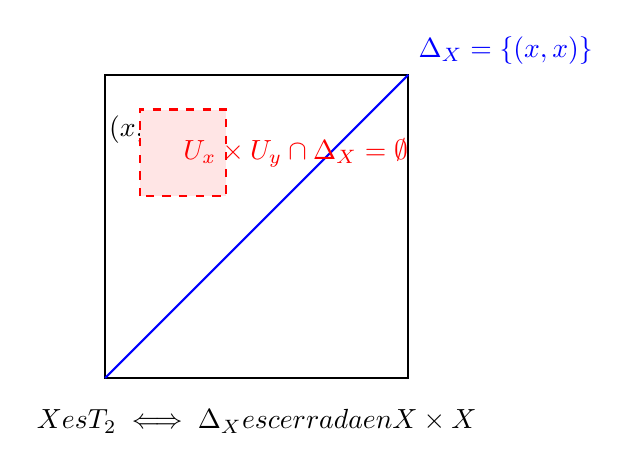
\begin{tikzpicture}[scale=1.1]
    \draw[thick] (0,0) rectangle (3.5,3.5);
    \draw[thick,blue] (0,0) -- (3.5,3.5) node[above right] {\(\Delta_X = \{(x,x)\}\)};
    \filldraw[black] (0.9,2.6) circle (1.8pt) node[above left] {\((x, y)\)};
    \draw[dashed,red,thick,fill=red!10] (0.4,2.1) rectangle (1.4,3.1);
    \node[red] at (2.2,2.6) {\(U_x \times U_y \cap \Delta_X = \emptyset\)};
    \node at (1.75,-0.5) {\(X \text{ es } T_2 \iff \Delta_X \text{ es cerrada en } X \times X\)};
\end{tikzpicture}
\end{center}

\begin{teo}[Teorema de Weierstrass de los valores extremos]
Sea \(K\) un espacio topológico compacto no vacío y \(f \colon K \to \mathbb{R}\) continua. Entonces \(f\) alcanza su máximo y su mínimo absolutos en \(K\).
\end{teo}

\begin{dem}
Por la Propiedad 1.3, la imagen \(f(K) \subseteq \mathbb{R}\) es compacta. Por el Teorema de Heine-Borel en \(\mathbb{R}\), \(f(K)\) es un subconjunto cerrado y acotado de \(\mathbb{R}\). Al ser acotado y no vacío, existen \(M := \sup f(K)\) y \(m := \inf f(K)\) en \(\mathbb{R}\). Por ser \(f(K)\) cerrado, se verifica que \(M \in f(K)\) y \(m \in f(K)\). Por tanto, existen puntos \(x_{\max}, x_{\min} \in K\) tales que:
\[
    f(x_{\max}) = M = \max_{x \in K} f(x), \qquad f(x_{\min}) = m = \min_{x \in K} f(x).
\]
\end{dem}
\end{comment}